\documentclass[sigconf]{acmart}
\usepackage{booktabs} % For formal tables
\usepackage{hyperref}
\usepackage{graphicx}
\usepackage{amsmath, bm}
\usepackage{float}
\usepackage{upgreek}
\usepackage{amssymb}
\settopmatter{printacmref=false} % Removes citation information below abstract

\renewcommand\footnotetextcopyrightpermission[1]{} % removes footnote with conference information in first column
\pagestyle{plain} % removes running headers





\begin{document}

\title{Comp6212 Computational Finance - 2017/18 Assignment (Part I)}
%\subtitle{2017/18, Assignment (Part I)}
\titlenote{GitHub Link: \url{https://github.com/Trouble404/Computational-Finance-coursework}}
%\titlenote{Website link:\url{https://d2v4olxsjbfep7.cloudfront.net/}}
\author{Junming Zhang}
\affiliation{%
    \institution{Electronics and Computer Science - Data Science}
    \institution{University of Southampton}
    \institution{Southampton, United Kingdom}
    \institution{Student ID: 29299527}
}
\email{jzlg17@ecs.soton.ac.uk}


%
\maketitle
\section{(A) 25 Marks}
\subsection{Question 1}
\[
\bm{m}=\begin{bmatrix}
0.10\\ 
0.10
\end{bmatrix} \quad
C = \begin{bmatrix}
 0.005 & 0.0\\ 
 -0.0& 0.005 
\end{bmatrix}
\]

\begin{itemize}
\item Portfolio with highest return with unconstrained risk:
\begin{equation} \label{eq0_1}
\mathcal{L} = \pi^{T}\bm{m} - \lambda(\sum_{i=1}^{2}\pi_{i}-1)
\end{equation}

\begin{equation} \label{eq0_2}
\frac{\partial \mathcal{L}}{\partial \pi_{(1,2)}} = \pi_{(1,2)} - \lambda = 0
\end{equation}

\begin{equation} \label{eq0_3}
\frac{\partial \mathcal{L}}{\partial \lambda} = -(\sum_{i=1}^{2}\pi_{i}-1) = 0
\end{equation}

The sum of portfolio should be 1, therefore, $\pi_{max\ return(1,2)} = [0.5,0.5]$ can be calculate by eq\eqref{eq0_2} and eq\eqref{eq0_3}. ~\\

\item Portfolio with the lowest variance with unconstrained by expectation:

\begin{equation} \label{eq0_4}
\mathcal{L} = \frac{1}{2}\pi^{T}C\pi - \lambda(\sum_{i=1}^{2}\pi_{i}-1) = \frac{1}{2}(0.005(\pi_{1}^{2}+\pi_{2}^{2}) - \lambda(\sum_{i=1}^{2}\pi_{i}-1)
\end{equation}

\begin{equation} \label{eq0_5}
\frac{\partial \mathcal{L}}{\partial \pi_{(1,2)}} = 0.005\pi_{(1,2)} - \lambda = 0
\end{equation}

The sum of portfolio should be 1, therefore, $\pi_{min\ variance(1,2)} = [0.5,0.5]$ can be calculate by eq\eqref{eq0_5} and eq\eqref{eq0_3}. ~\\

\end{itemize}

Hence, the return of two portfolio should be $R_{(1,2)} = \pi^{T}\bm{m} = [0.1,0.1]$ which is the efficent frontier point.
%%%%%%%%%%%%%%%%%%%%%%%%%%%%%%%%%%%%%%%%%%%%%%5

\subsection{Question 2}

\[
\bm{m}=\begin{bmatrix}
0.10\\ 
0.20\\ 
0.15
\end{bmatrix} \quad
C = \begin{bmatrix}
 0.005 & -0.010 & 0.004\\ 
 -0.010& 0.040 & \\ -0.002
 0.004& -0.002 & 0.023
\end{bmatrix}
\]

  E-V space is using expected return as the x-axis and standard deviation as the y-axis. Suppose 3 assets A1, A2 and A3 with expected return $\bm{m}$ and covariance matrix $C$. 100 random portfolios can be generated by the matrix with random elements and analyzed by following parameters: 

\begin{itemize}
\item Portfolio weight $X$ with $ \sum_{i=1}^{3}X_{i}=1$
\item Expected return $E=\sum_{i=1}^{3}X_{i}\mu_{i}$
\item Expected variance $V=\sum_{i=1}^{3}X_{i}X_{j}\sigma_{ij}$
\end{itemize}

  And the scatter diagram of 100 random portfolios can be plotted in the E-V space which is shown in $Fig.1$.

\begin{figure}[htbp]
%\setlength{\abovecaptionskip}{0.cm}
%\setlength{\belowcaptionskip}{-0.cm}
    \centering
    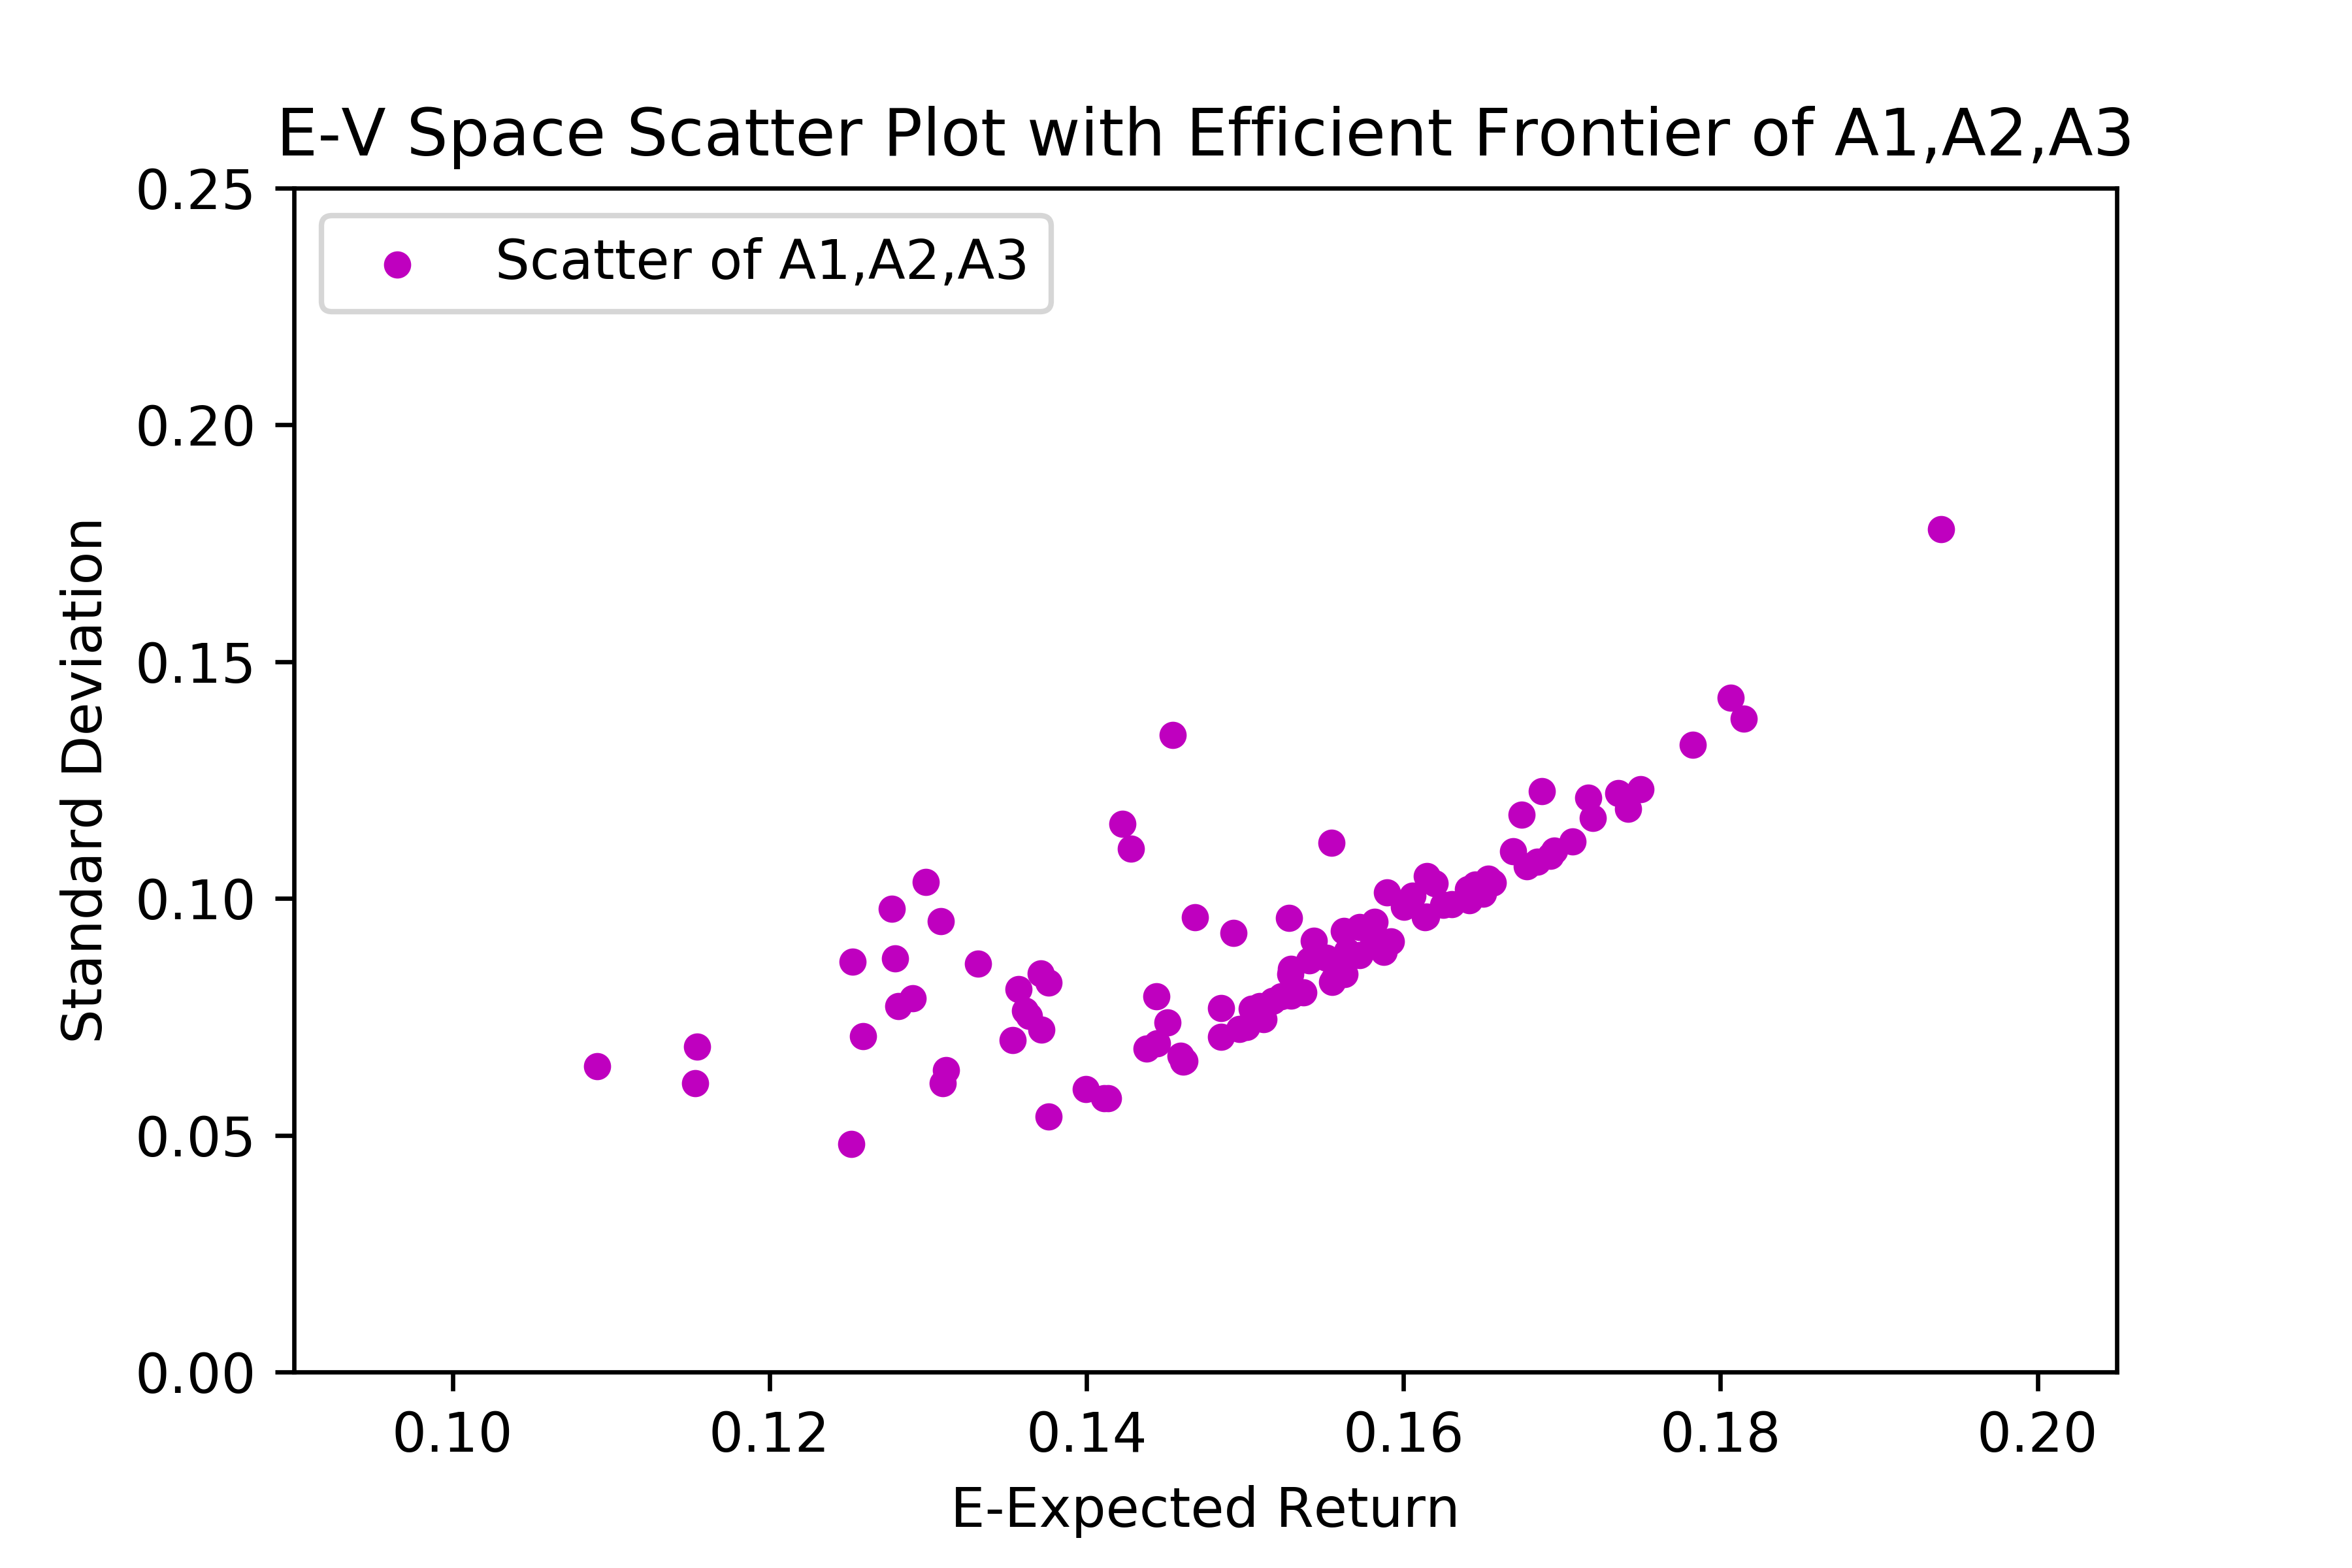
\includegraphics[width=0.5\textwidth]{1.png}
    \caption{\label{}E-V Space Scatter Plot of A1,A2,A3}
\end{figure}

\[
  \bm{m_{12}}=\begin{bmatrix}
0.10\\ 
0.20 
\end{bmatrix} \quad \bm{m_{13}}=\begin{bmatrix}
0.10\\ 
0.15 
\end{bmatrix} \quad   \bm{m_{23}}=\begin{bmatrix}
0.20\\ 
0.15 
\end{bmatrix}
\]

\[
C_{12}=\begin{bmatrix}
0.005 & -0.010\\ 
-0.010 & 0.040 
\end{bmatrix} \quad C_{13}=\begin{bmatrix}
0.005 & 0.004\\ 
0.004 & 0.023
\end{bmatrix} \quad   C_{23}=\begin{bmatrix}
0.040 & -0.002\\ 
-0.002 & 0.023 
\end{bmatrix}
\]

Similarly, the expected return and standard deviation of 3 pair-wise assets A1A2, A1A3 and A2A3 can be calculated with previous equations.
The efficient portfolio frontier for these 4 assets can be plotted by $\bm{plotFrontier}$ function in MATLAB's financial toolbox. Those frontiers are shown in $Fig2$. It could find the standard deviation will increase with the expected return. However, different combinations of portfolios will cause different return and risk. Elements in $C_{13}$ are all positive and it has lower return with higher risk which means it is not a good portfolio selection. Other 3 assets have similar efficient frontiers but according to the curvature, A1A2A3 has the lowest risk with the highest return. Therefore, the core thought of asset portfolio is to disperse the portfolio selection for preventing individual risk. 

\begin{figure}[htbp]
    \centering
    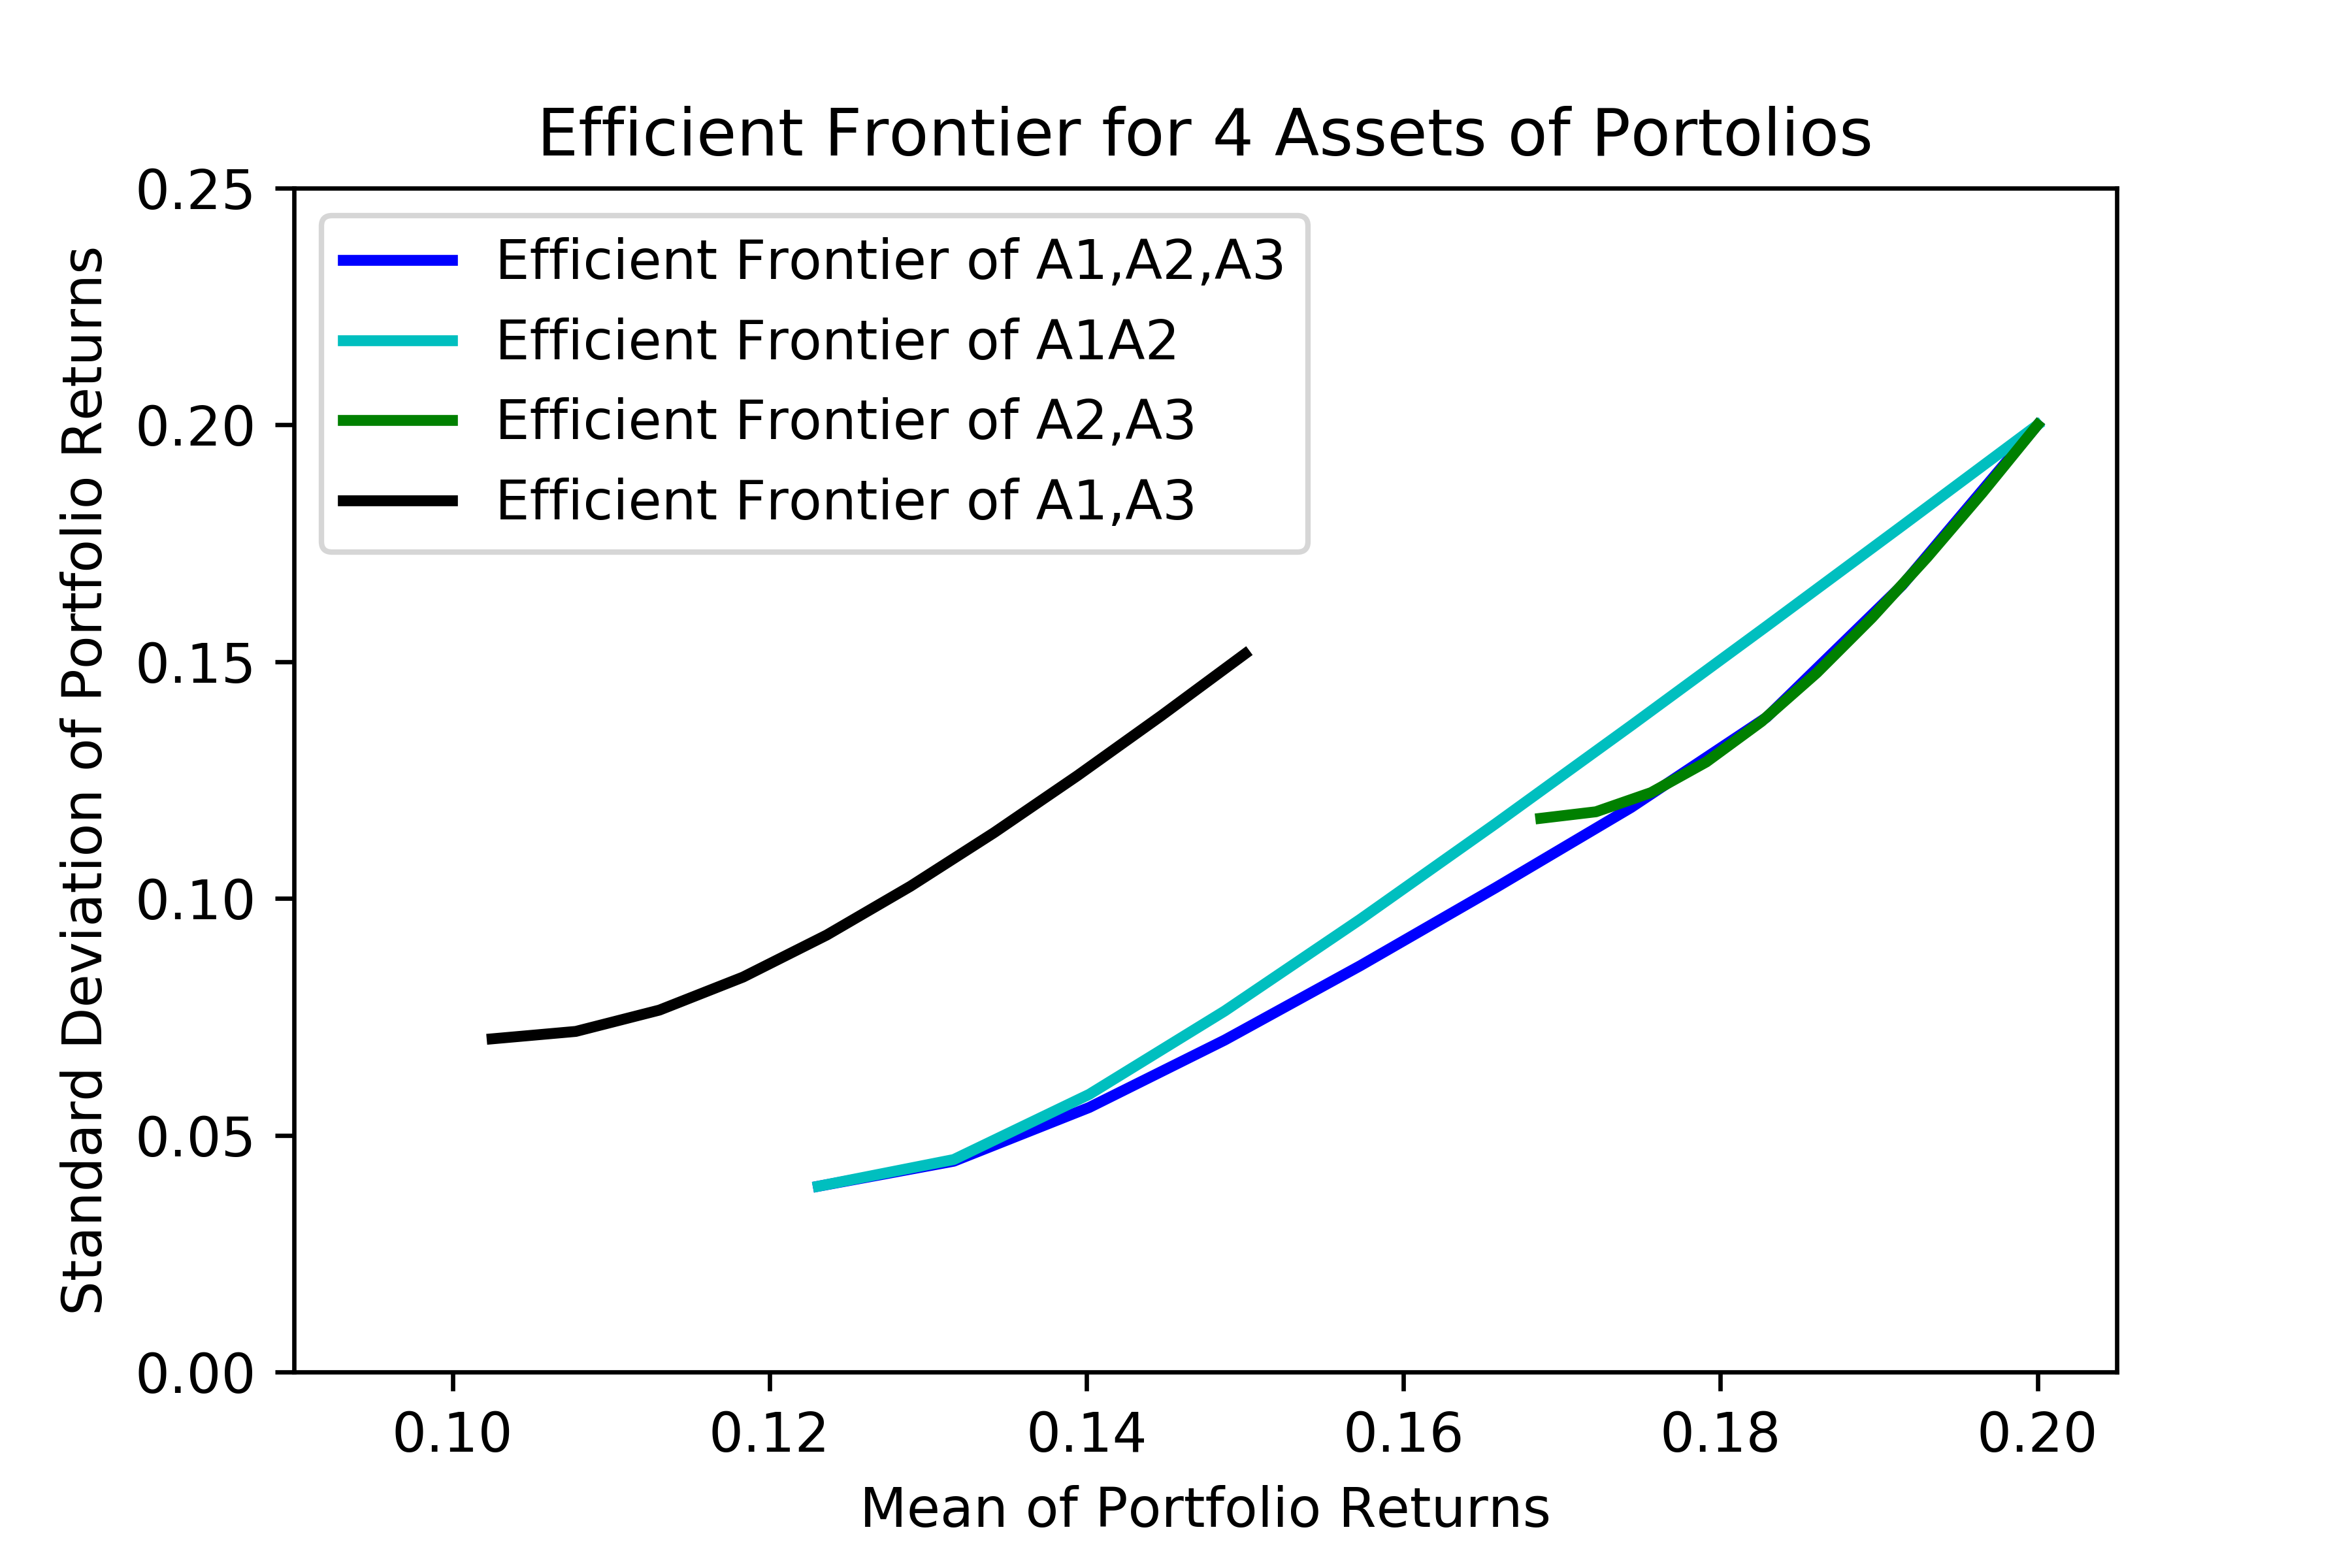
\includegraphics[width=0.5\textwidth]{2.png}
    \caption{\label{}Efficient Frontier for 4 Assets of Portolios}
\end{figure}

%%%%%%%%%%%%%%%%%%%%%%%%%%%%%%%%%%%%%%%%%%%%%%%%%%%%%%%%%%%%%%%%%%%%%%%%%%%%%%%%%%%%%%%%%

\subsection{Question 3}

The CVX toolbox can be installed by running $csv\_setup.m$ in MATLAB according to set the working directory to the cvx folder of the Matlab installed address. 

The efficient frontier can be plotted by $NativeMV$ function, it will generate the efficient frontier by two efficient portfolios which have maximizing return and minimizing risk.

Portfolio with highest return with unconstrained risk can be defined as expected return $\mu$. 

\begin{equation} \label{eq1}
\setlength{\abovedisplayskip}{3pt}
\setlength{\belowdisplayskip}{3pt}
max\,\bm{\pi}^{T}\bm{\mu}\ subject\ to\ \sum_{i=1}^{N}\pi_{i}=1\ and\ \bm{\pi_{i}}\geq 0.
\end{equation}

 $linprog$ is used to solve this problem and it could be defined as: 

\begin{equation} \label{eq2}
\setlength{\abovedisplayskip}{3pt}
\setlength{\belowdisplayskip}{3pt}
\min \limits_{x}\,\bm{f^{T}}\bm{x}\ such\ that\ \left\{\begin{matrix}
\bm{Ax}\leqslant \bm{b}
\\ \bm{A}_{eq}\bm{x}=\bm{b}_{eq}
\\ lb\leqslant \bm{x}\leqslant ub
\end{matrix}\right.
\end{equation}

Following code are used to replace $linprog(f,A,b,A_{eq},b_{eq},lb,ub)$ to CVX method:

\begin{figure}[htbp]
    \centering
    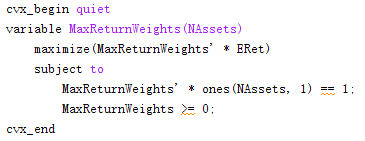
\includegraphics[width=0.4\textwidth]{3.png}
    %\caption{\label{}Efficient Frontier of NativeMV and CVX}
\end{figure}

Portfolio with the lowest variance with unconstrained by expectation can be defined as expected covariance $\Sigma$.

\begin{equation} \label{eq3}
\setlength{\abovedisplayskip}{3pt}
\setlength{\belowdisplayskip}{3pt}
min\,\bm{\pi}^{T}\bm{\Sigma}\bm{\pi}\ subject\ to\ \sum_{i=1}^{N}\pi_{i}=1.
\end{equation}

$quadprog$ is used to obtain minimum varaiances with respective $\bm{r}_{tar}$. And it could be defined as:

\begin{equation} \label{eq4}
\setlength{\abovedisplayskip}{3pt}
\setlength{\belowdisplayskip}{3pt}
min\,\bm{\pi}^{T}\bm{\Sigma}\bm{\pi}\ subject\ to\ \sum_{i=1}^{N}\pi_{i}=1 ,\ \bm{\pi_{i}} \geqslant 0 \ and\ \bm{\pi}^{T}\bm{\mu}=\bm{r}_{tar}
\end{equation}

Following code are used to replace $quadprog$ to CVX method:

\begin{figure}[htbp]
    \centering
    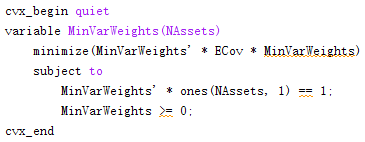
\includegraphics[width=0.4\textwidth]{4.png}
    %\caption{\label{}Efficient Frontier of NativeMV and CVX}
\end{figure}

Therefore, the efficient frontier of the portfolio with $\bm{m}$ and $C$ can be plotted by two methods, $Fig3$ shows two frontiers in the same scale and it could found the result is almost same. $Fig4$ is the difference between two frontiers, the difference value is extremely small because the scale of x and y axis is smaller than $10^-7$. 

\begin{figure}[htbp]
    \centering
    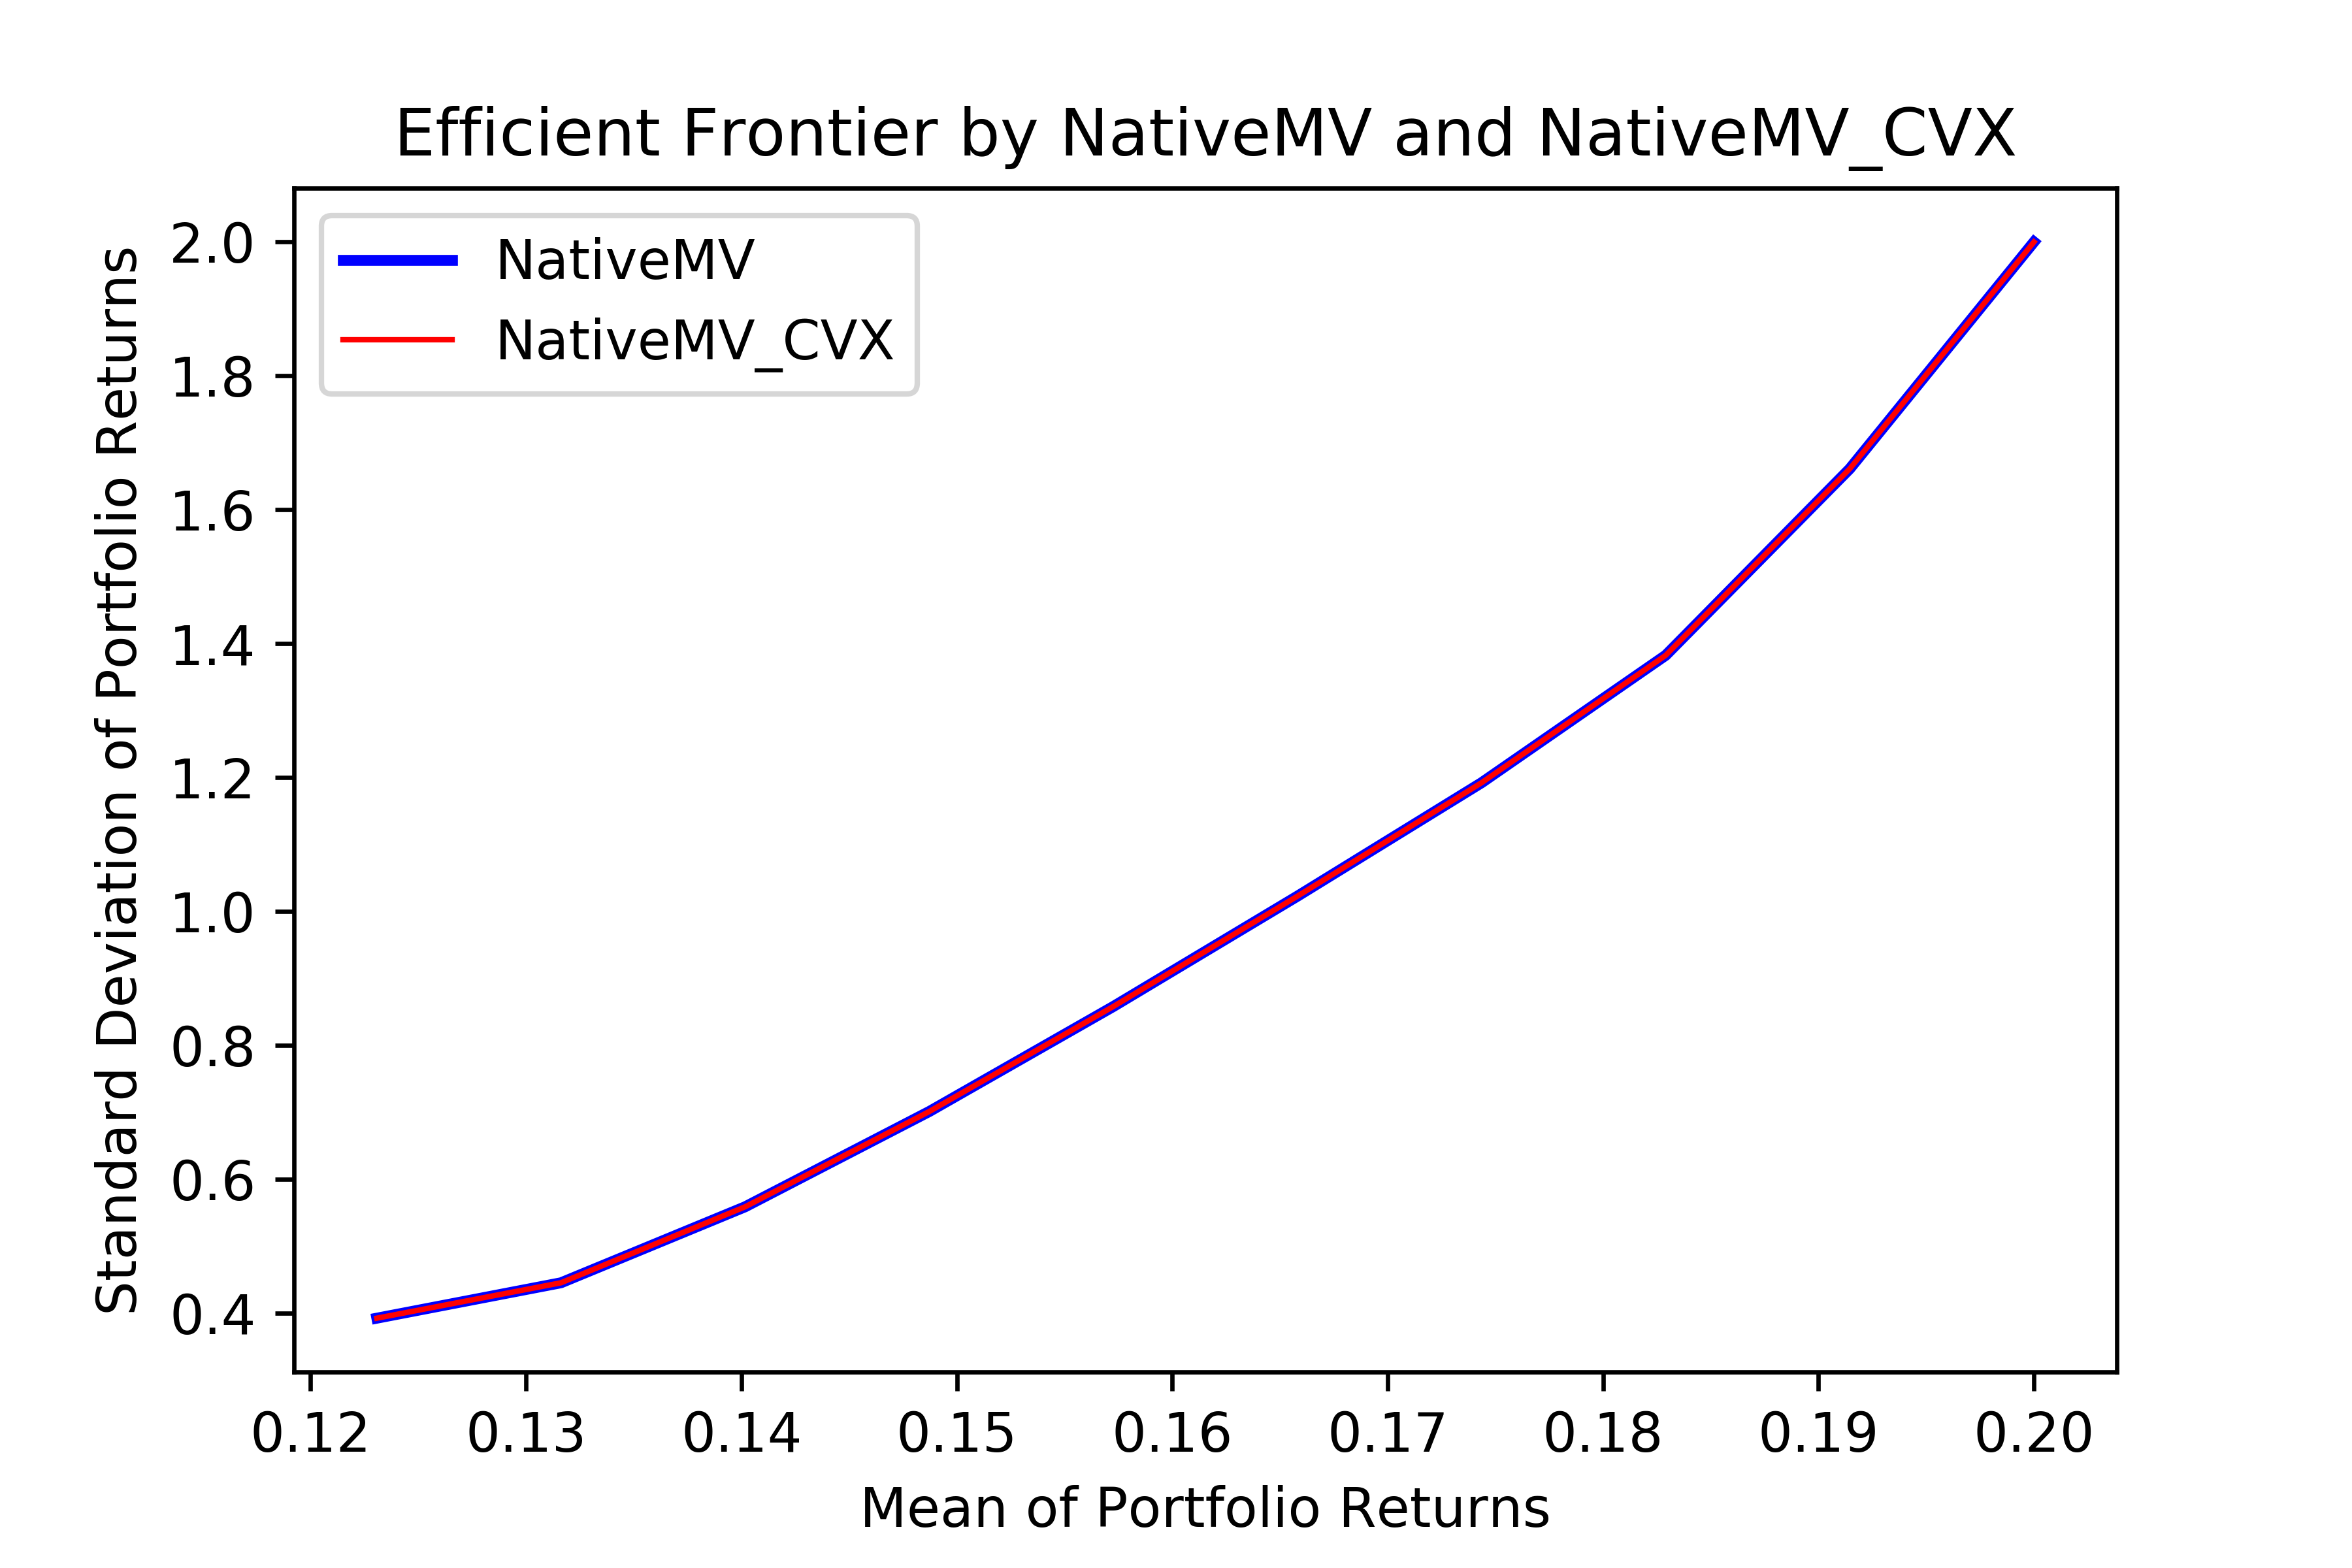
\includegraphics[width=0.5\textwidth]{5.png}
    \caption{\label{}Efficient Frontier of NativeMV and CVX}
\end{figure}

\begin{figure}[htbp]
    \centering
    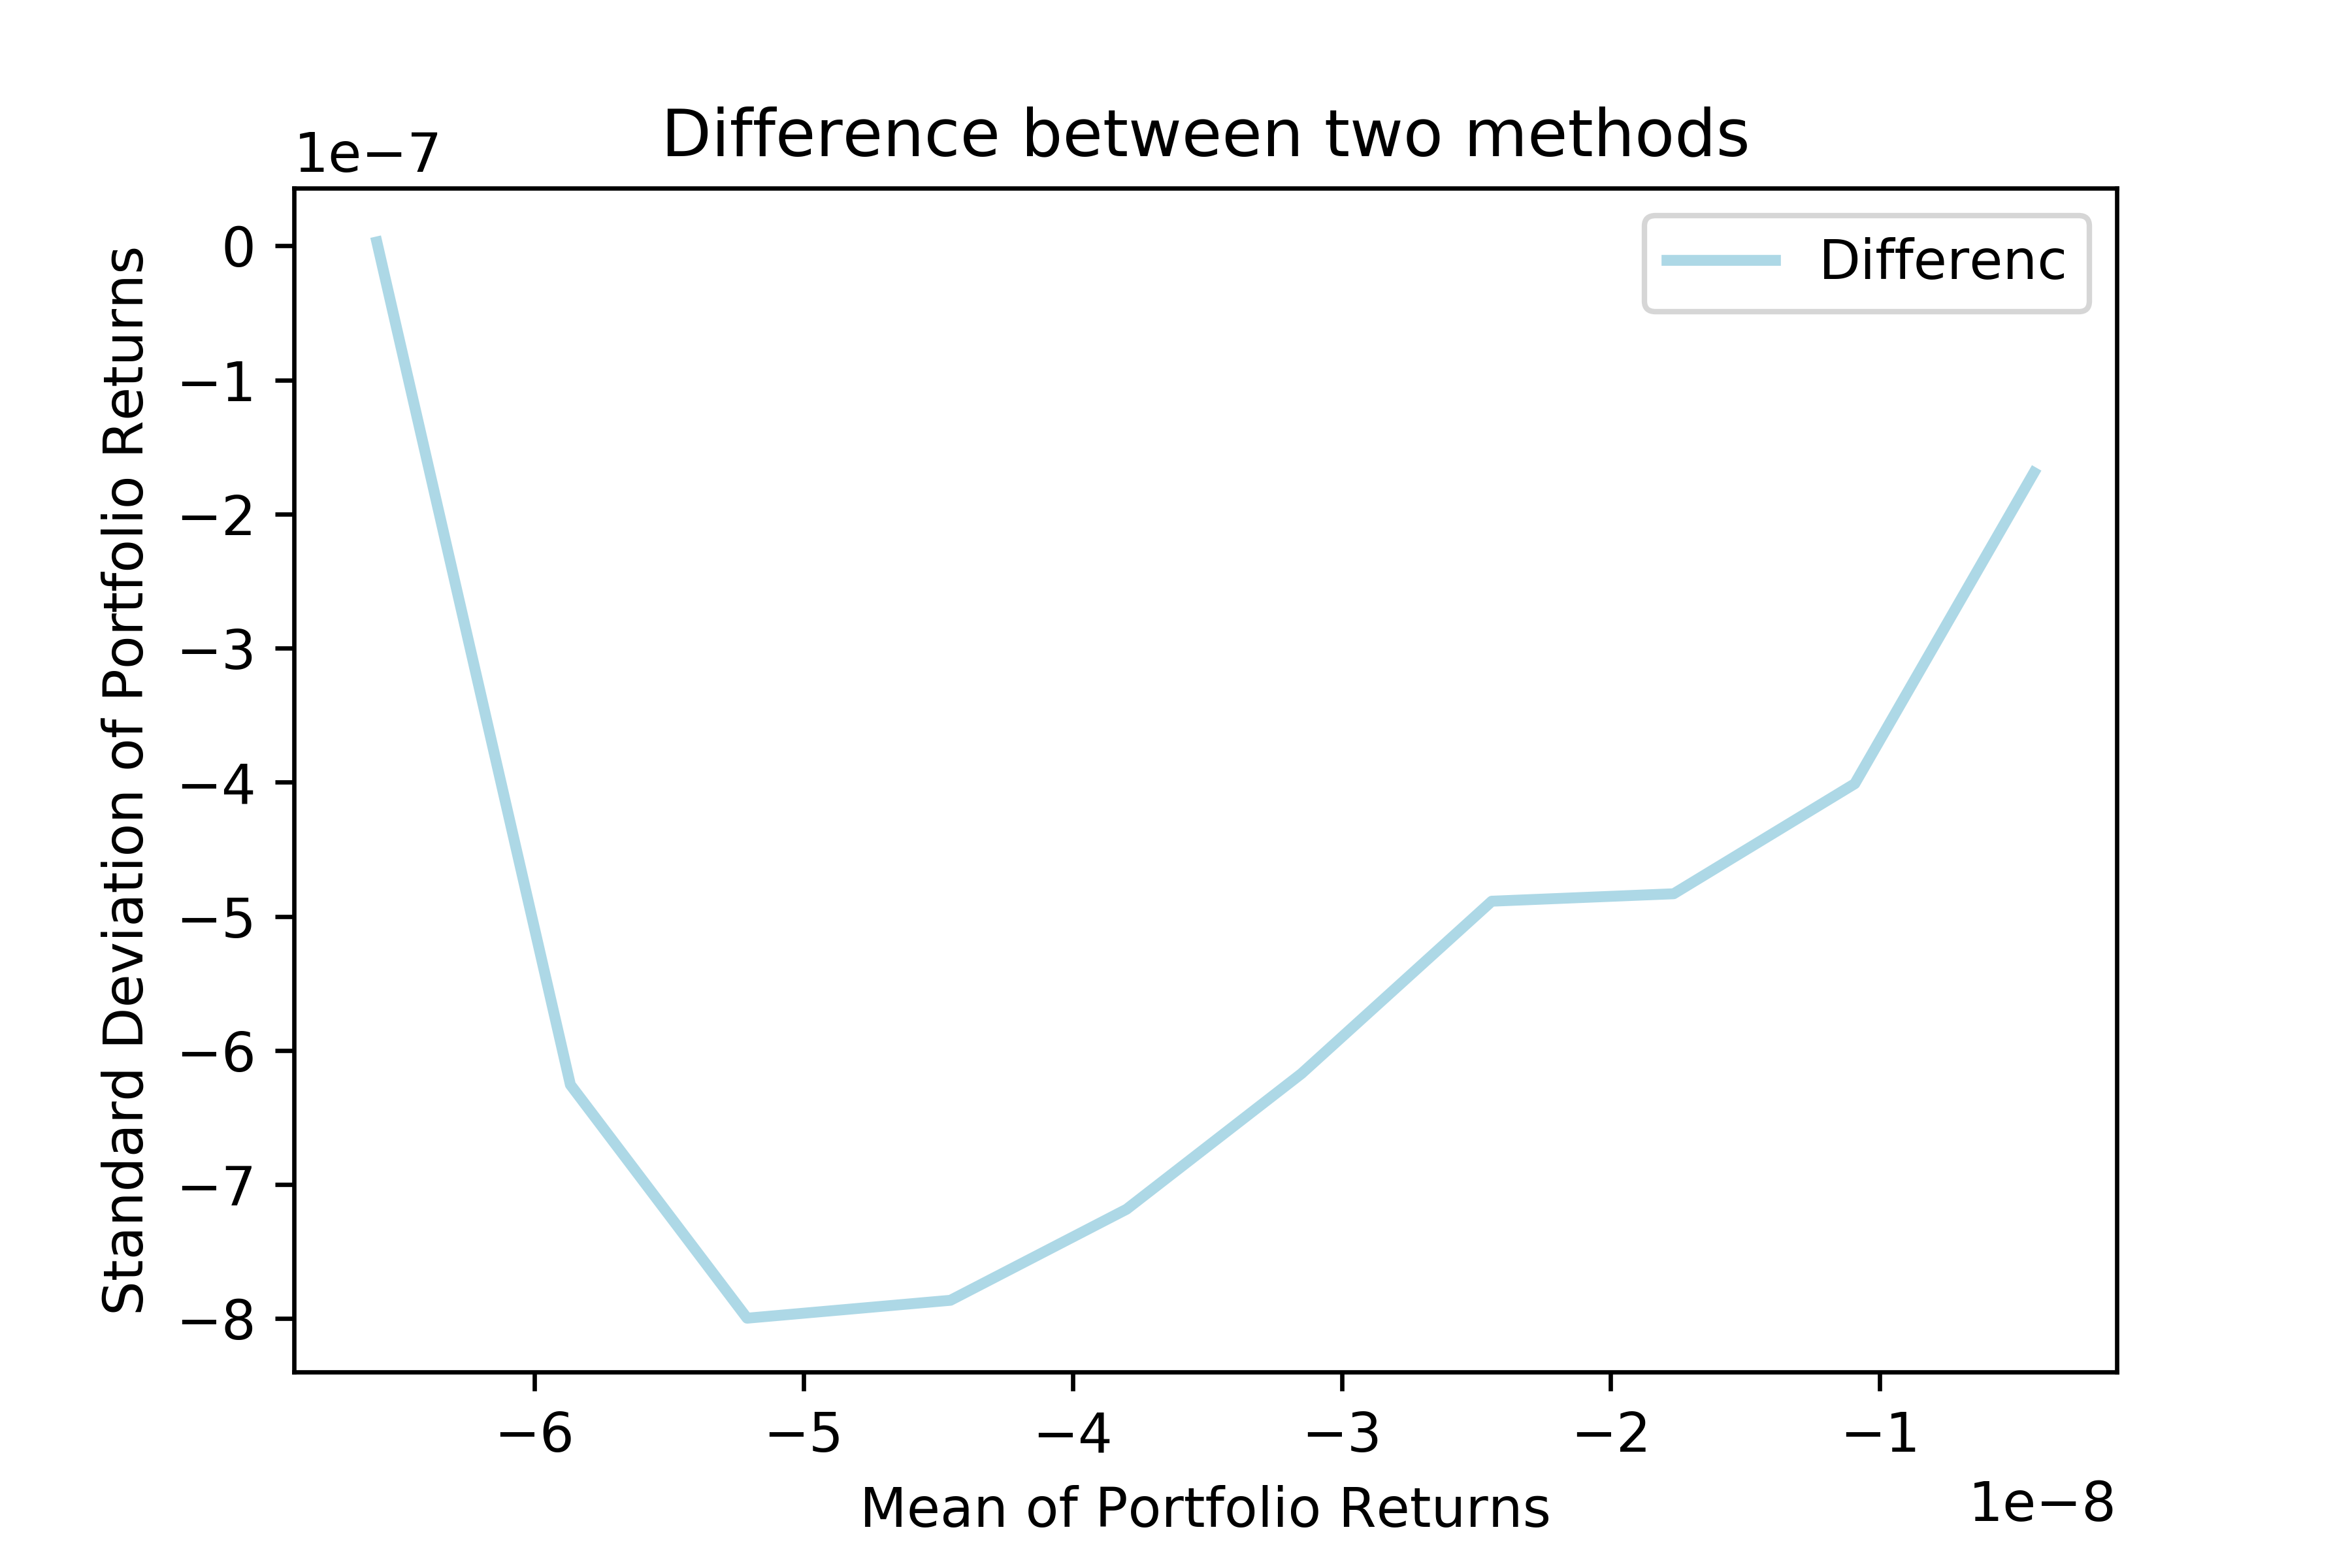
\includegraphics[width=0.5\textwidth]{6.png}
    \caption{\label{}Difference between frontiers of NativeMV and CVX}
\end{figure}

%%%%%%%%%%%%%%%%%%%%%%%%%%%%%%%%%%%%%%%%%%%%%%%%%%%%%%%%%%%%%%%%%%%%%%%%%%%%%%%%%%%%%%%%%

\subsection{Question 4}\label{q4}

FTSE 100 historical data of 30 companies from 21/02/2015 to 21/02/2018 are obtained in $Yahoo Finance$. Most of them contain data of 759 workdays, missing data were filled by the predicted data with time serise. Return of those 30 companies in 3 years will be calculated by $R = close\ price - open\ price$. In this case, the return data will be a $759\times30$ matrix.

3 stocks are chosen by random numbers $[10\ 22\ 25]$, and the expected returns $m$ and covariances $C$ of them will be estimated by the first half of time series which is 379 workdays.

\begin{equation} \label{eq5}
\setlength{\abovedisplayskip}{3pt}
\setlength{\belowdisplayskip}{3pt}
\hat{m}_{(10,22,25)} = \frac{1}{T} \sum_{t=1}^{379} R_{(10,22,25)}(t) = \begin{bmatrix}
-2.3628&-0.6702&0.1966
\end{bmatrix}
\end{equation}

\begin{equation} \label{eq6}
\setlength{\abovedisplayskip}{3pt}
\setlength{\belowdisplayskip}{3pt}
\begin{split}
\hat{C}_{(10,22,25)} = \frac{1}{T} \sum_{t=1}^{379} (R_{(10,22,25)}(t)-\hat{m})^{T}(R_{(10,22,25)}(t)-\hat{m}) \\
= \begin{bmatrix}
649.9110 & 71.3647 & 171.0259\\
71.3647 & 255.4663 & 108.3973\\
171.0259 & 108.3973 & 240.9117
\end{bmatrix}
\end{split}
\end{equation}

Then the CVX toolbox will be used to find the best weight by Markowitz portfolio method, based on eq\eqref{eq4} without shortsale constrained, the highest value in m is 0.1966, therefore, a smaller expected return 0.18 is chosen to calculate the weights. In this case, it will obtain a portfolio weight $\bm{w}_{Markowitz} = \begin{bmatrix}-0.1097&0.3430&0.7667\end{bmatrix}$. The nagative weight means shortsale of stocks.

In addition, a naive $\frac{1}{N}$ portfolio method will be used to do a comparison with Markowitz portfolio method. In this case, the weight based on this strategy will be $\bm{w}_{\frac{1}{N}} = \begin{bmatrix}\frac{1}{3}&\frac{1}{3}&\frac{1}{3}\end{bmatrix}$.

Based on the conclusion in ``Optimal Versus Naive Diversification: How Inefficient is the $\frac{1}{N}$ Portfolio Strategy?'', the $out-of-sample$ Sharpe ratio of mean-variance strategy is much lower than the $\frac{1}{N}$ strategy and there is no single model that delivers a Sharpe ratio or a CEQ return higher than $\frac{1}{N}$ method\cite{demiguel2007optimal}.

In this question, the real return and Sharpe ratio will be used to compare the performance of these two strategies.

\begin{equation} \label{eq7}
\begin{split}
\setlength{\abovedisplayskip}{3pt}
\setlength{\belowdisplayskip}{3pt}
Real\ return_{(Markowitz,\frac{1}{N}strategy)} = [-158.7126,75.5333]\\
sum(R_{(10,22,25)} \times \bm{w}_{Markowitz,\frac{1}{N}strategy})
\end{split}
\end{equation}

\begin{equation} \label{eq8}
\setlength{\abovedisplayskip}{3pt}
\setlength{\belowdisplayskip}{3pt}
\begin{split}
Sharpe\ ratio_{(Markowitz,\frac{1}{N}strategy)} = [-0.0367,0.0161]\\
\frac{mean(Real\ return_{(Markowitz,\frac{1}{N}strategy)})-free\ risk}{std(Real\ return_{(Markowitz,\frac{1}{N}strategy)})}
\end{split}
\end{equation}

Assuming the risk-free ratio is 2\%, it could find the performance of $\frac{1}{N}$ is better than Markowitz in this case which is similar to the previous conclusion. However, that paper also pointed out that different optimizing models will have a better performance when the mean and variance are calculated from plenty of assets and enough period\cite{demiguel2007optimal}. In this question, it is not enough to obtain a good result with data from 3 assets and 379 workdays.

\begin{figure}[htbp]
    \centering
    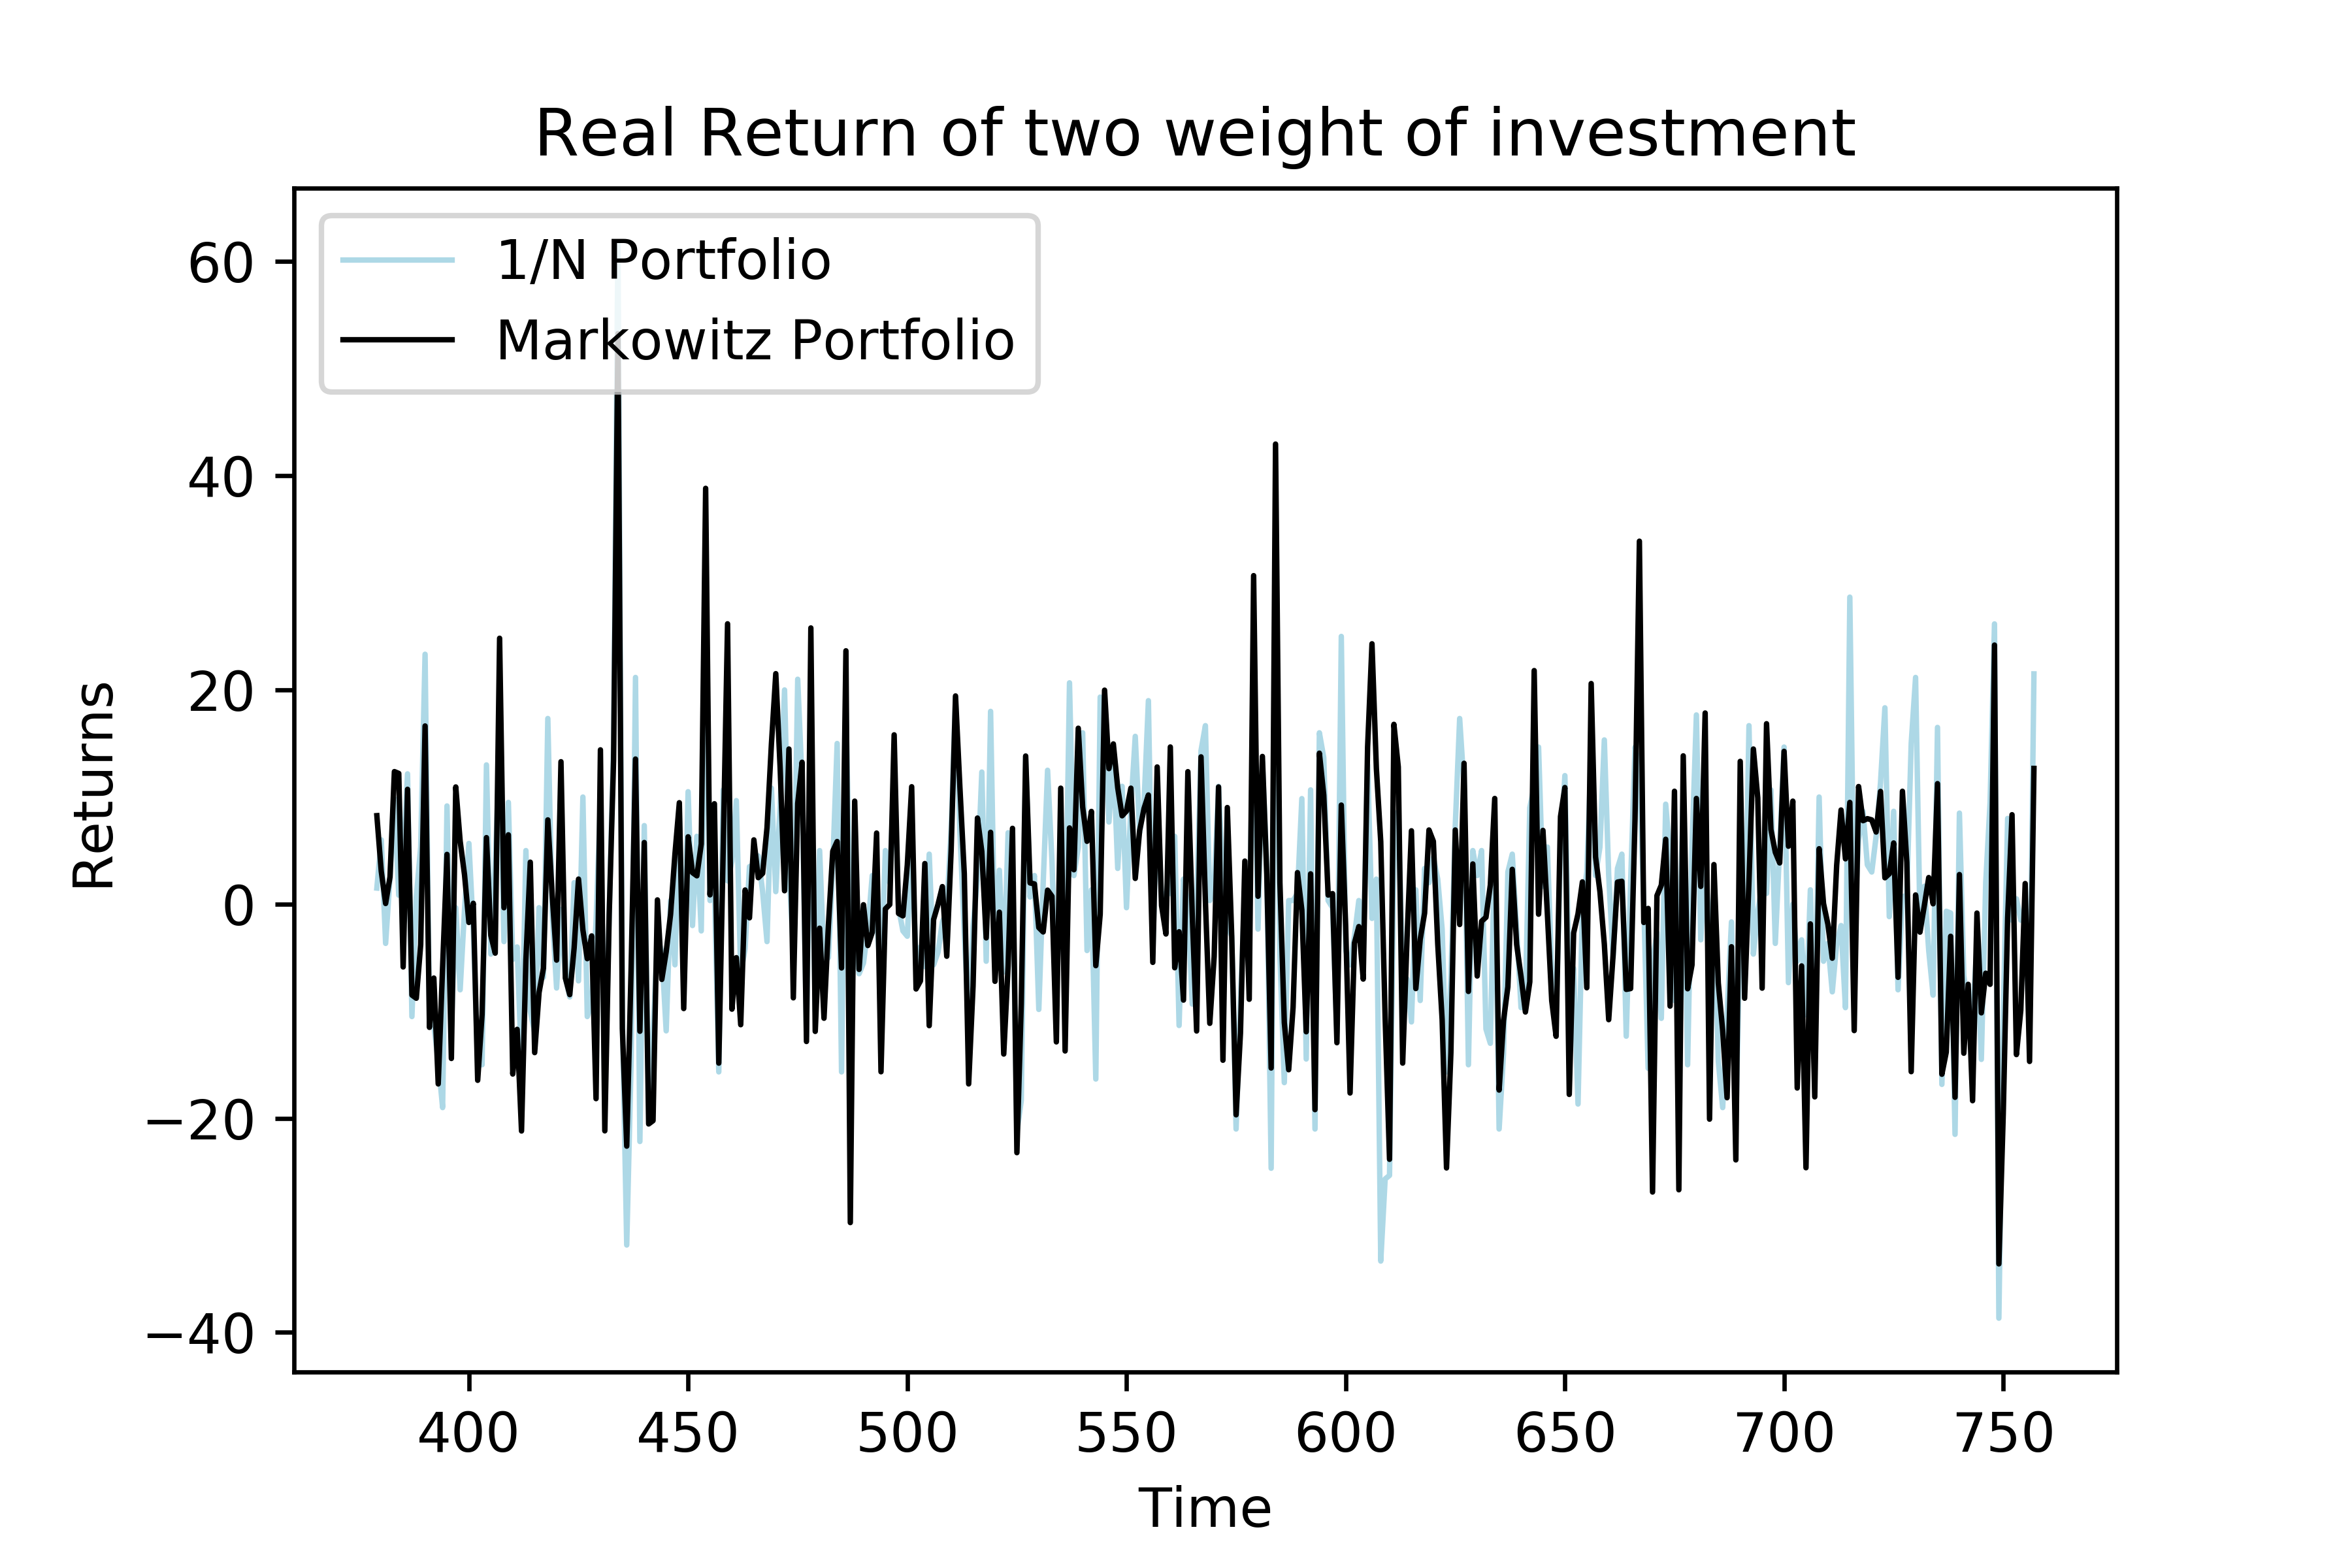
\includegraphics[width=0.5\textwidth]{7.png}
    \caption{\label{}Real Return of two stragegies comparasion}
\end{figure}

%%%%%%%%%%%%%%%%%%%%%%%%%%%%%%%%%%%%%%%%%%%%%%%%%%%%%%%%%%%%%%%%%%%%%%%%%%%%%%%%%%%%%%%%%

\subsection{Question 5}

The Short sale means investors sell borrowed stocks, they will make money if the stock goes down in price but lose money when the price goes up. Therefore, the short sale-constrained portfolios mean the portfolio's weight should be positive. However this method is not allowed in some countries, therefore, this part will foucs on shortsale constrained portfolios.


In this case, covariance $\hat{C}_{(10,22,25)}$ is an non-singular matrix bacause the value of determinant is not 0. Therefore, it is defined as eq\eqref{eq4}, and the best weight could be calculated by Lagrangian method in which $\lambda_{t}$ is $N\times1$ vector of Lagrange multipliers for the constraints on shortselling\cite{tian2016primal}:

\begin{equation} \label{eq9}
\setlength{\abovedisplayskip}{3pt}
\setlength{\belowdisplayskip}{3pt}
\mathcal{L} = x_{t}^{T}-\frac{\gamma}{2}x_{t}^{T}\Sigma_{t}+x_{t}^{T}\lambda_{t}
\end{equation}

\begin{equation} \label{eq10}
\setlength{\abovedisplayskip}{3pt}
\setlength{\belowdisplayskip}{3pt}
x^{*}=x_{1}+r_{0}x_{2}
\end{equation}

\begin{equation} \label{eq11}
\setlength{\abovedisplayskip}{3pt}
\setlength{\belowdisplayskip}{3pt}
x_{1}=\frac{1}{\Delta}(c(V^{-1}\bm{1}_{N})-b(V^{-1}r))
\end{equation}

\begin{equation} \label{eq12}
\setlength{\abovedisplayskip}{3pt}
\setlength{\belowdisplayskip}{3pt}
x_{2}=\frac{1}{\Delta}(a(V^{-1}r)-b(V^{-1}\bm{1}_{N}))
\end{equation}

The optimal solution of this model can be obtained as eq\eqref{eq10} with eq\eqref{eq11} and eq\eqref{eq12}. In addition, $a=\bm{1}_{N}V^{-1}\bm{1}_{N}$, $b=\bm{1}_{N}V^{-1}r$, $c=r^{T}V^{-1}r$ and $\Delta=ac-b^{2}$. It could find the solution of portfolios in non-singular matrix is one special condition in singular matrix.

Then the CVX toolbox will be used to find the best weight by Markowitz portfolio method, based on eq\eqref{eq4}, the highest value in m is 0.1966, therefore, a smaller expected return 0.18 is chosen to calculate the weights. In this case, it will obtain a portfolio weight $\bm{w}_{Shortsale-constrained} = \begin{bmatrix}0&0.0191&0.9809\end{bmatrix}$.

The real return eq\eqref{eq7} is $[-68.0340]$ and Sharpe ratio eq\eqref{eq8} is $[-0.0172]$. 

It could find the perfomance of short selling constrained portfolio is higher than short selling permitting portfolio in this case. In addtion, the difference between them is that most optimal solutions in the first condition has non zero value which means most properties are considered to use. But in short selling constrained condition, lost of the optimal solution is 0, stocks which have negative return will obtain approximate 0 portfolio weight.


%%%%%%%%%%%%%%%%%%%%%%%%%%%%%%%%%%%%%%%%%%%%%%%%%%%%%%%%%%%%%%%%%%%%%%%%%%%%%%%%%%%%%%%%%

\subsection{Question 6}

Index-Tracking refers to use a portfolio of stocks to replicate the index of the market and obtain similar returns of the index by minimizing the tracking errors. In general, it focuses on minimizing the variance and transaction costs of stocks with relevant portfolio returns.

\begin{equation} \label{eq13}
\setlength{\abovedisplayskip}{3pt}
\setlength{\belowdisplayskip}{3pt}
\min \limits_{w}\left \| \bm{y}-\bm{Rw} \right \|_{2}^{2}
\end{equation}

FTSE 100 historical data of 30 companies had obtained in \nameref{q4} and represented as a $759\times30$ matrix $R\_30$. In this part, the extra data of FTSE 100 index is obtained from $YahooFinance$ and a $759\times1$ matrix $y\_1$ can be calculated as the return of FTSE 100 index. 6 stocks which are fifth of available stocks will be selected by Greedy forward selection algorithm and Sparse index tracking by $l_{1}$ regularization. In addition, the minimum tracking error can be defined as \eqref{eq13}.

\begin{itemize}
\item \textbf{Greedy forward selection algorithm}

A greedy algorithm is an algorithmic paradigm that follows the problem solving heuristic of making the locally optimal choice at each stage with the hope of finding a global optimum\cite{gutin2001introduction}.

\begin{figure}[htbp]
    \centering
    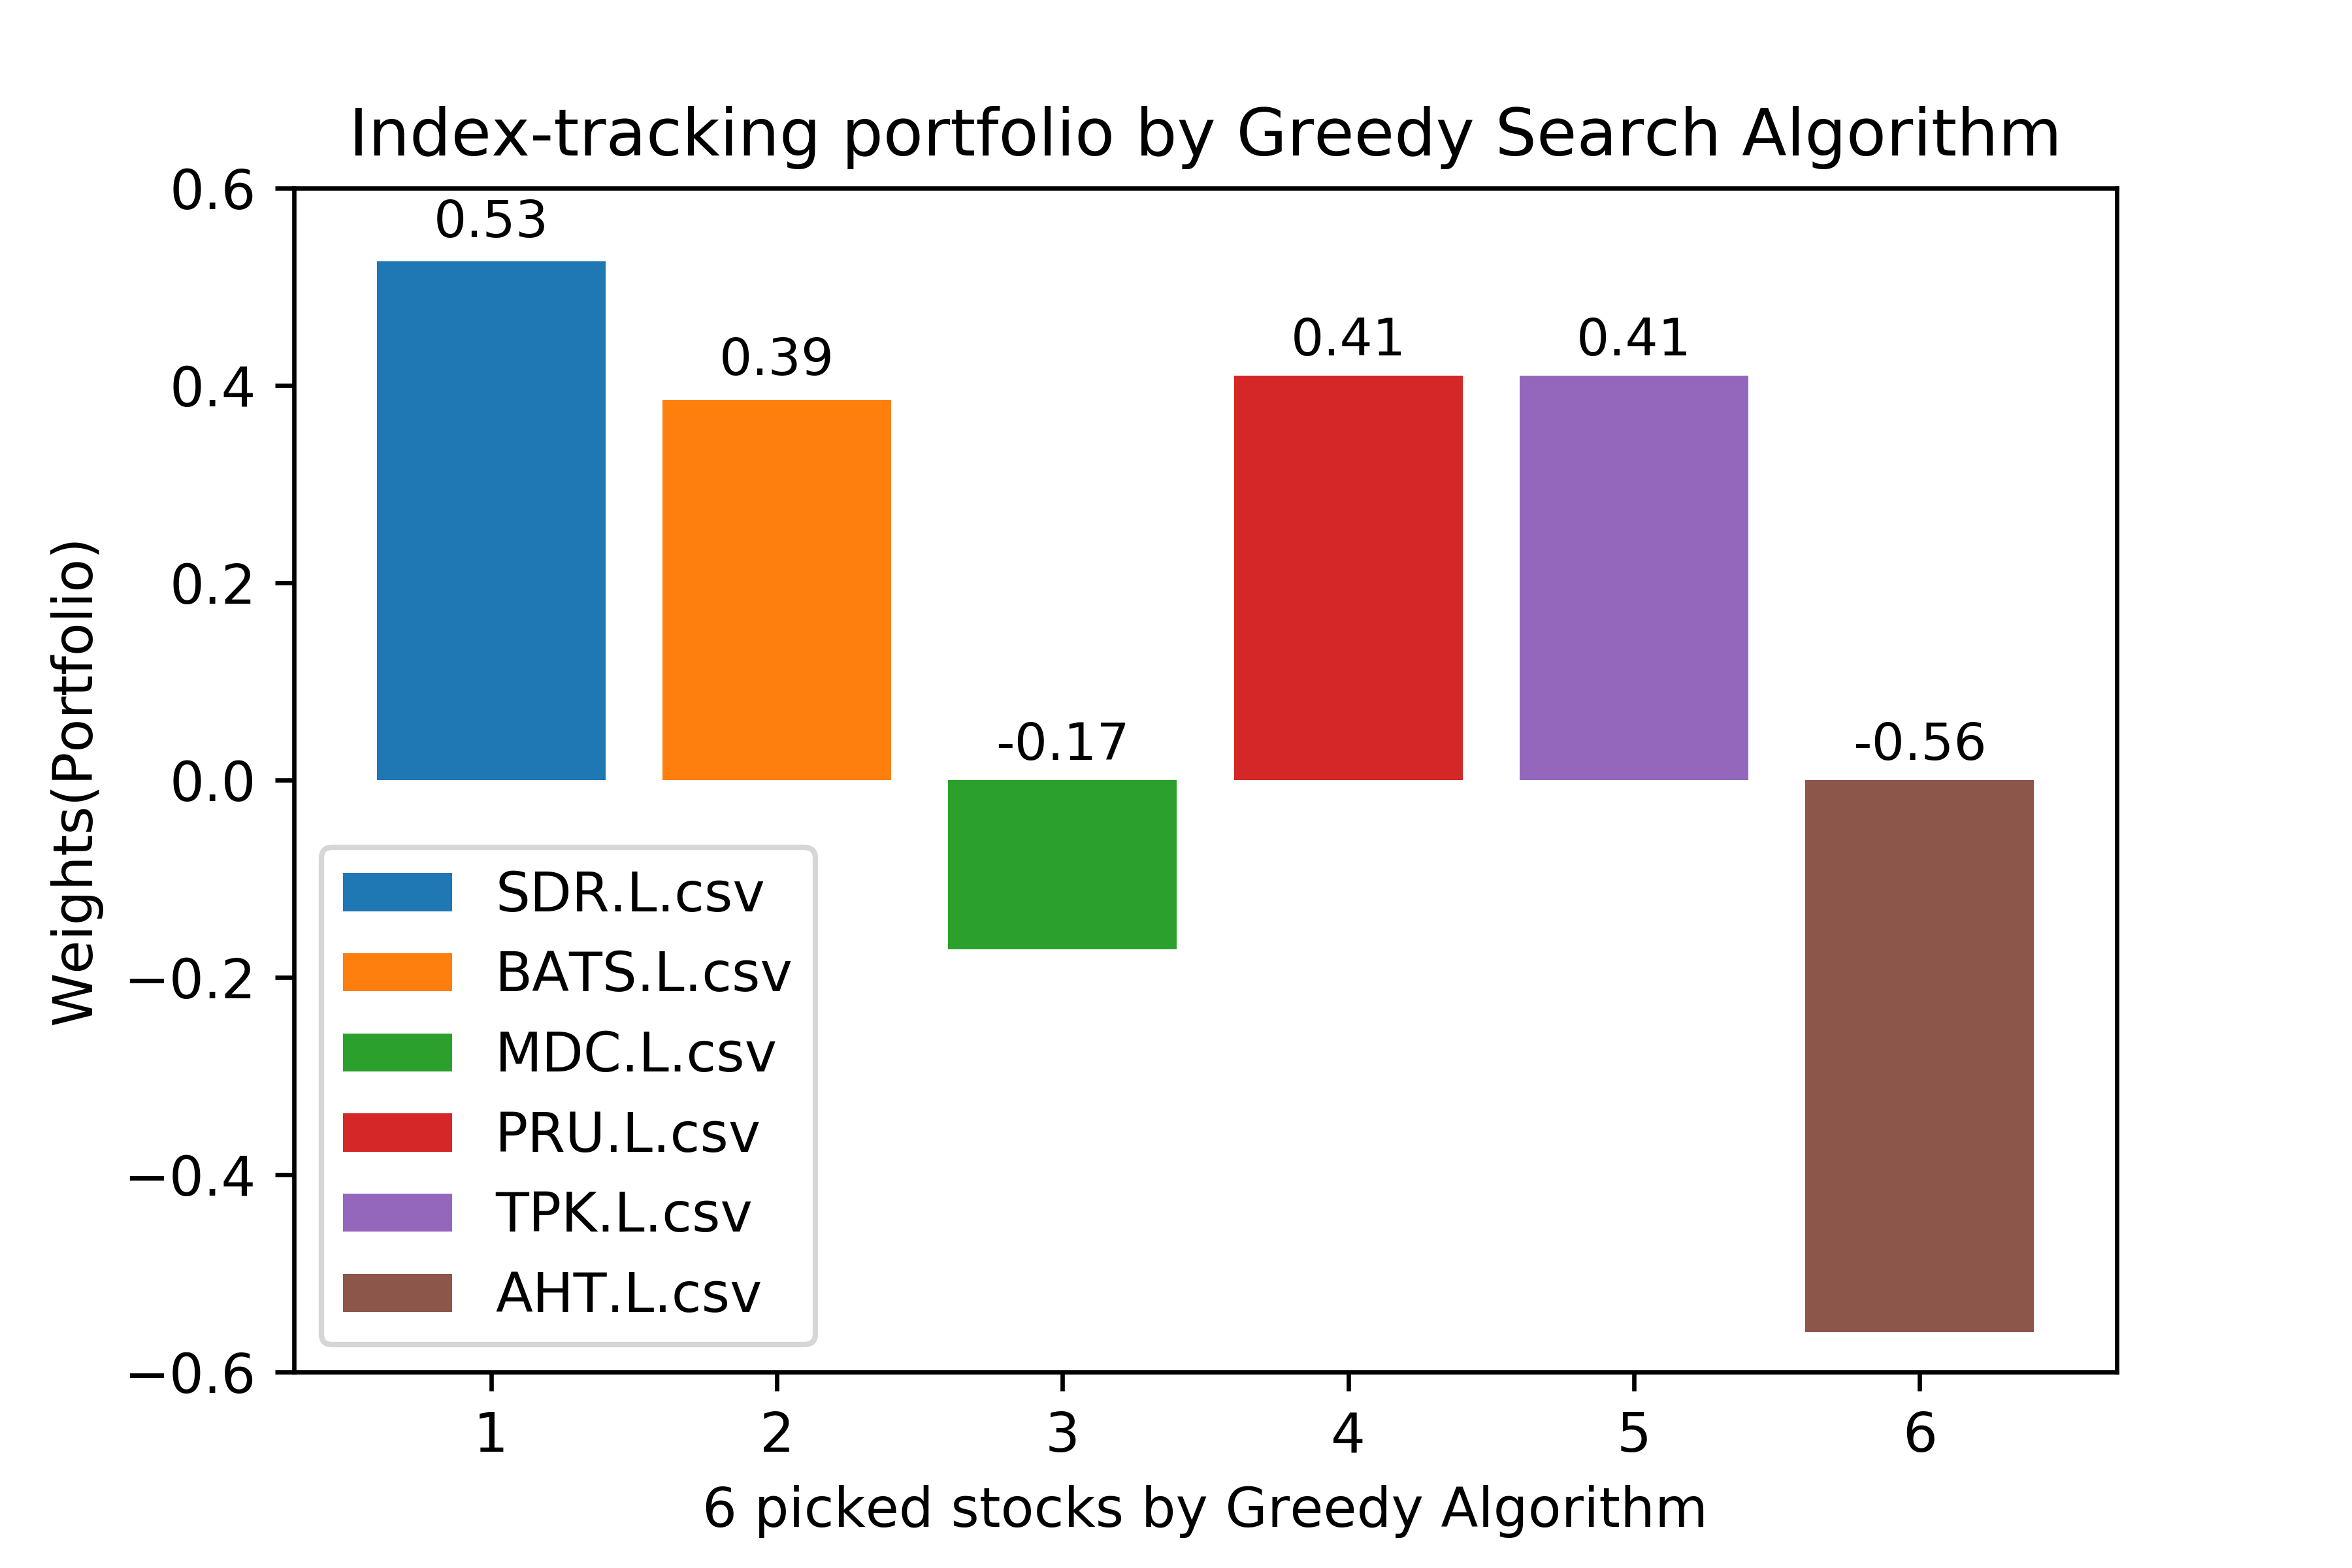
\includegraphics[width=0.5\textwidth]{8.png}
    \caption{\label{}Selected stocks by Greedy Algorithm}
\end{figure}

Stocks of 6 companies selection can be finished by 6 iterations by Greedy forward selection algorithm which is finding a new portfolio at each iteration to achieve the lowest tracking error with corresponding weights with \eqref{eq13}. The result is shown in $Fig6$.

Suppose the subset of selected stocks is $S$, the process of selection in this part is $S_{greedy}=[n_{19},n_{3},n_{14},n_{17},n_{26},n_{1}]$ and the corresponding weight is \\$w_{greedy}=[0.5256,0.3854,-0.1713,0.4099,0.4099,-0.5596]$ with mean squared error $2.1513$. ~\\


\item \textbf{Sparse index tracking using $\bm{l_{1}}$ regularization}

$L_{1}$ regularization is the sum of absolute value in the vector and sparse process can remove irrelevant features in elements to realize automatic selection. 

\begin{equation} \label{eq14}
\setlength{\abovedisplayskip}{3pt}
\setlength{\belowdisplayskip}{3pt}
\bm{w}^{[\uptau]}=arg\,\min\limits_{\bm{w}}[\left \| \bm{y}-\bm{Rw} \right \|_{2}^{2}+\uptau \sum_{i} \bm{s_{i}} \left |\bm{w_{i}}  \right |]
\end{equation}

\begin{equation} \label{eq15}
\setlength{\abovedisplayskip}{3pt}
\setlength{\belowdisplayskip}{3pt}
\bm{w}^{[\uptau]}=arg\,\min\limits_{\bm{w}}[\left \| \bm{y}-\bm{Rw} \right \|_{2}^{2}+\uptau \left \| \bm{w} \right \|_{1}] \ subject\ to\ \sum_{i=1}^{N}\bm{w_{i}}=1
\end{equation}

The equation of sparse index portfolio can be written as an optimized version eq\eqref{eq14} and a more general version eq\eqref{eq15}. a parameter $\uptau$ will be used to adjust the weight of $l_{1}$ penalization and $s_{i}$ is the transaction cost for the $i_{th}$ security\cite{brodie2009sparse}. In this case, eq\eqref{eq15} will be used to calculate the weights of selection by assuming all transaction costs are equal and adjusting the regularisation parameter $\uptau$ until the number of subsets is 6.

\begin{figure}[htbp]
    \centering
    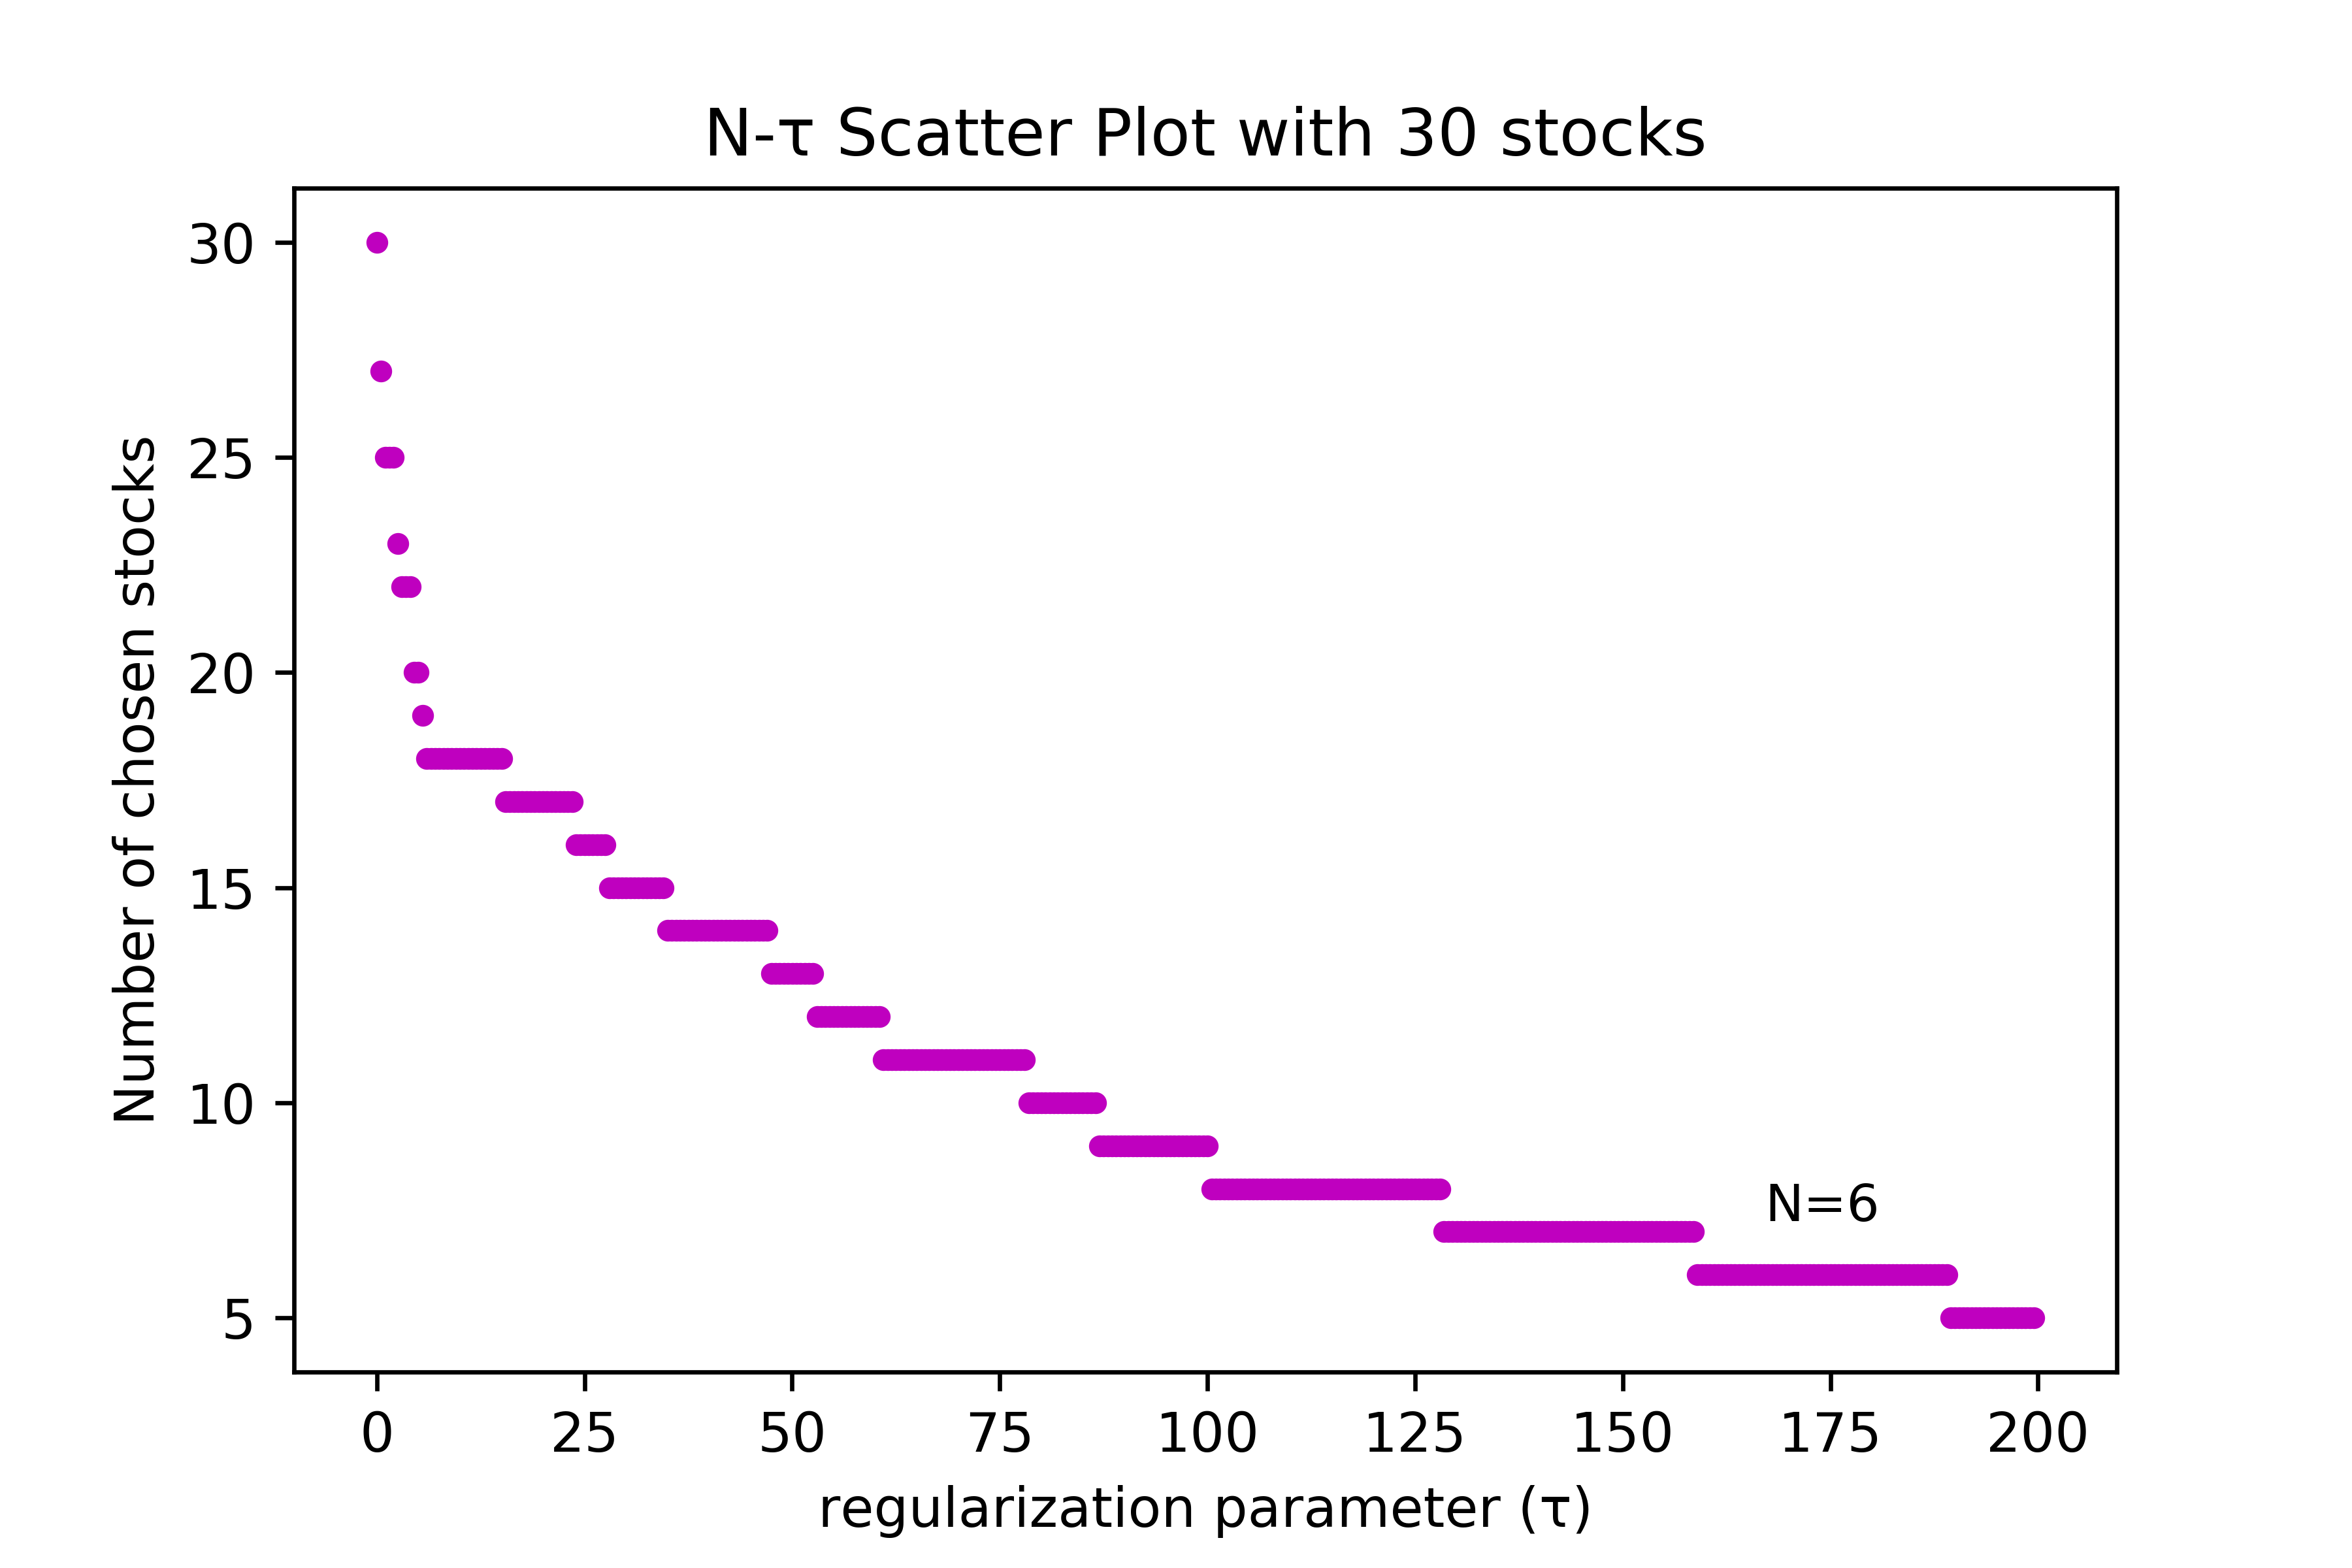
\includegraphics[width=0.5\textwidth]{9.png}
    \caption{\label{}The relationship between number of subsets and regularisation parameter}
\end{figure}

\begin{figure}[htbp]
    \centering
    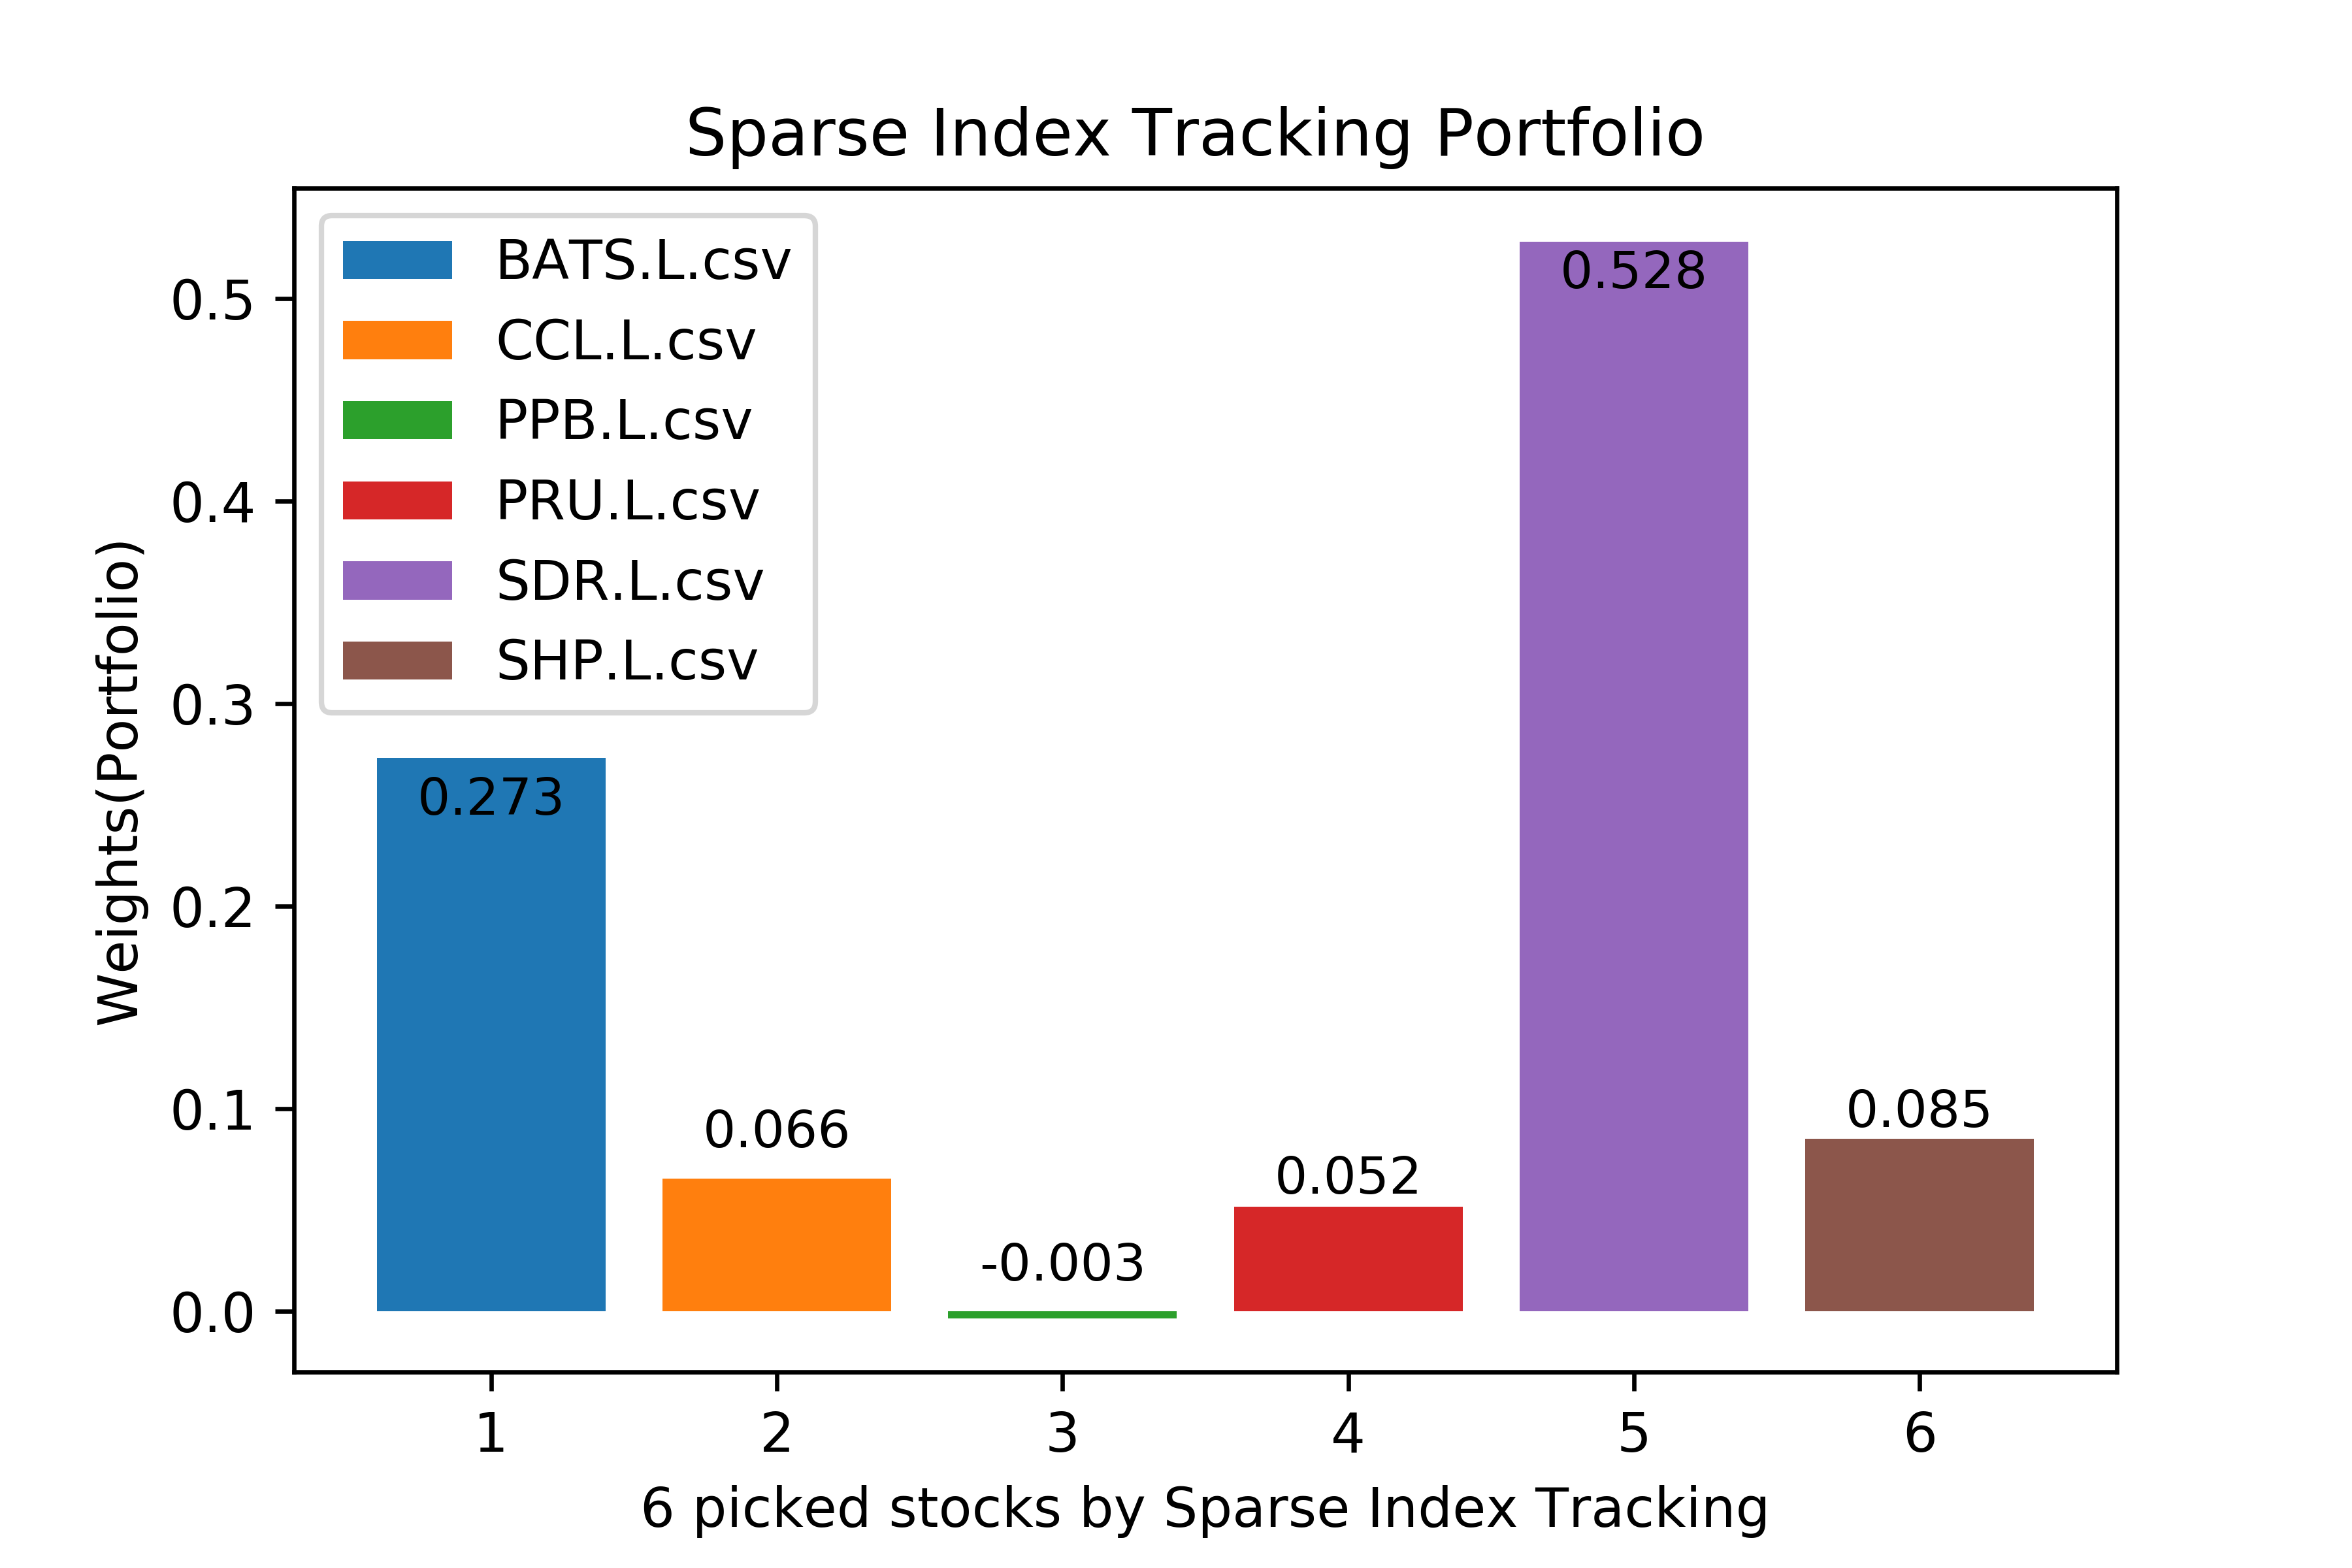
\includegraphics[width=0.5\textwidth]{10.png}
    \caption{\label{}Selected stocks by Sparse index tracking}
\end{figure}

To find the relationship between the number of subsets and regularisation parameter, 400 parameters with values between 0 to 200 were generated and applied to eq\eqref{eq15}. According to $Fig7$, it could find the centre point of 6 subsets is $\uptau=175$, therefore this value will be used to find 6 subsets which are $S_{sparse}=[n_{3},n_{6},n_{16},n_{17},n_{19},n_{20}]$ and corresponding weights $w_{sparse}=[0.2731,0.0656,-0.0033,0.0517,0.5278,0.0852]$ with mean squared error 1.8631. The result is shown in $Fig8$. ~\\

\end{itemize}

Due to the mean squared error is similar in two methods, their common selection $S_{common}=[n_{3},n_{17},n_{19}]$ should be considered as a better selection. The purpose of index tracking is to minimise the risk and the Sparse index tracking gives a lower error, however, the sum of actual return in two methods are $Sum\_R_{(greedy,sparse)}=[-117.5294,-202.5354]$ and it could find the Greedy algorithm gives a higher return.

\begin{figure}[htbp]
    \centering
    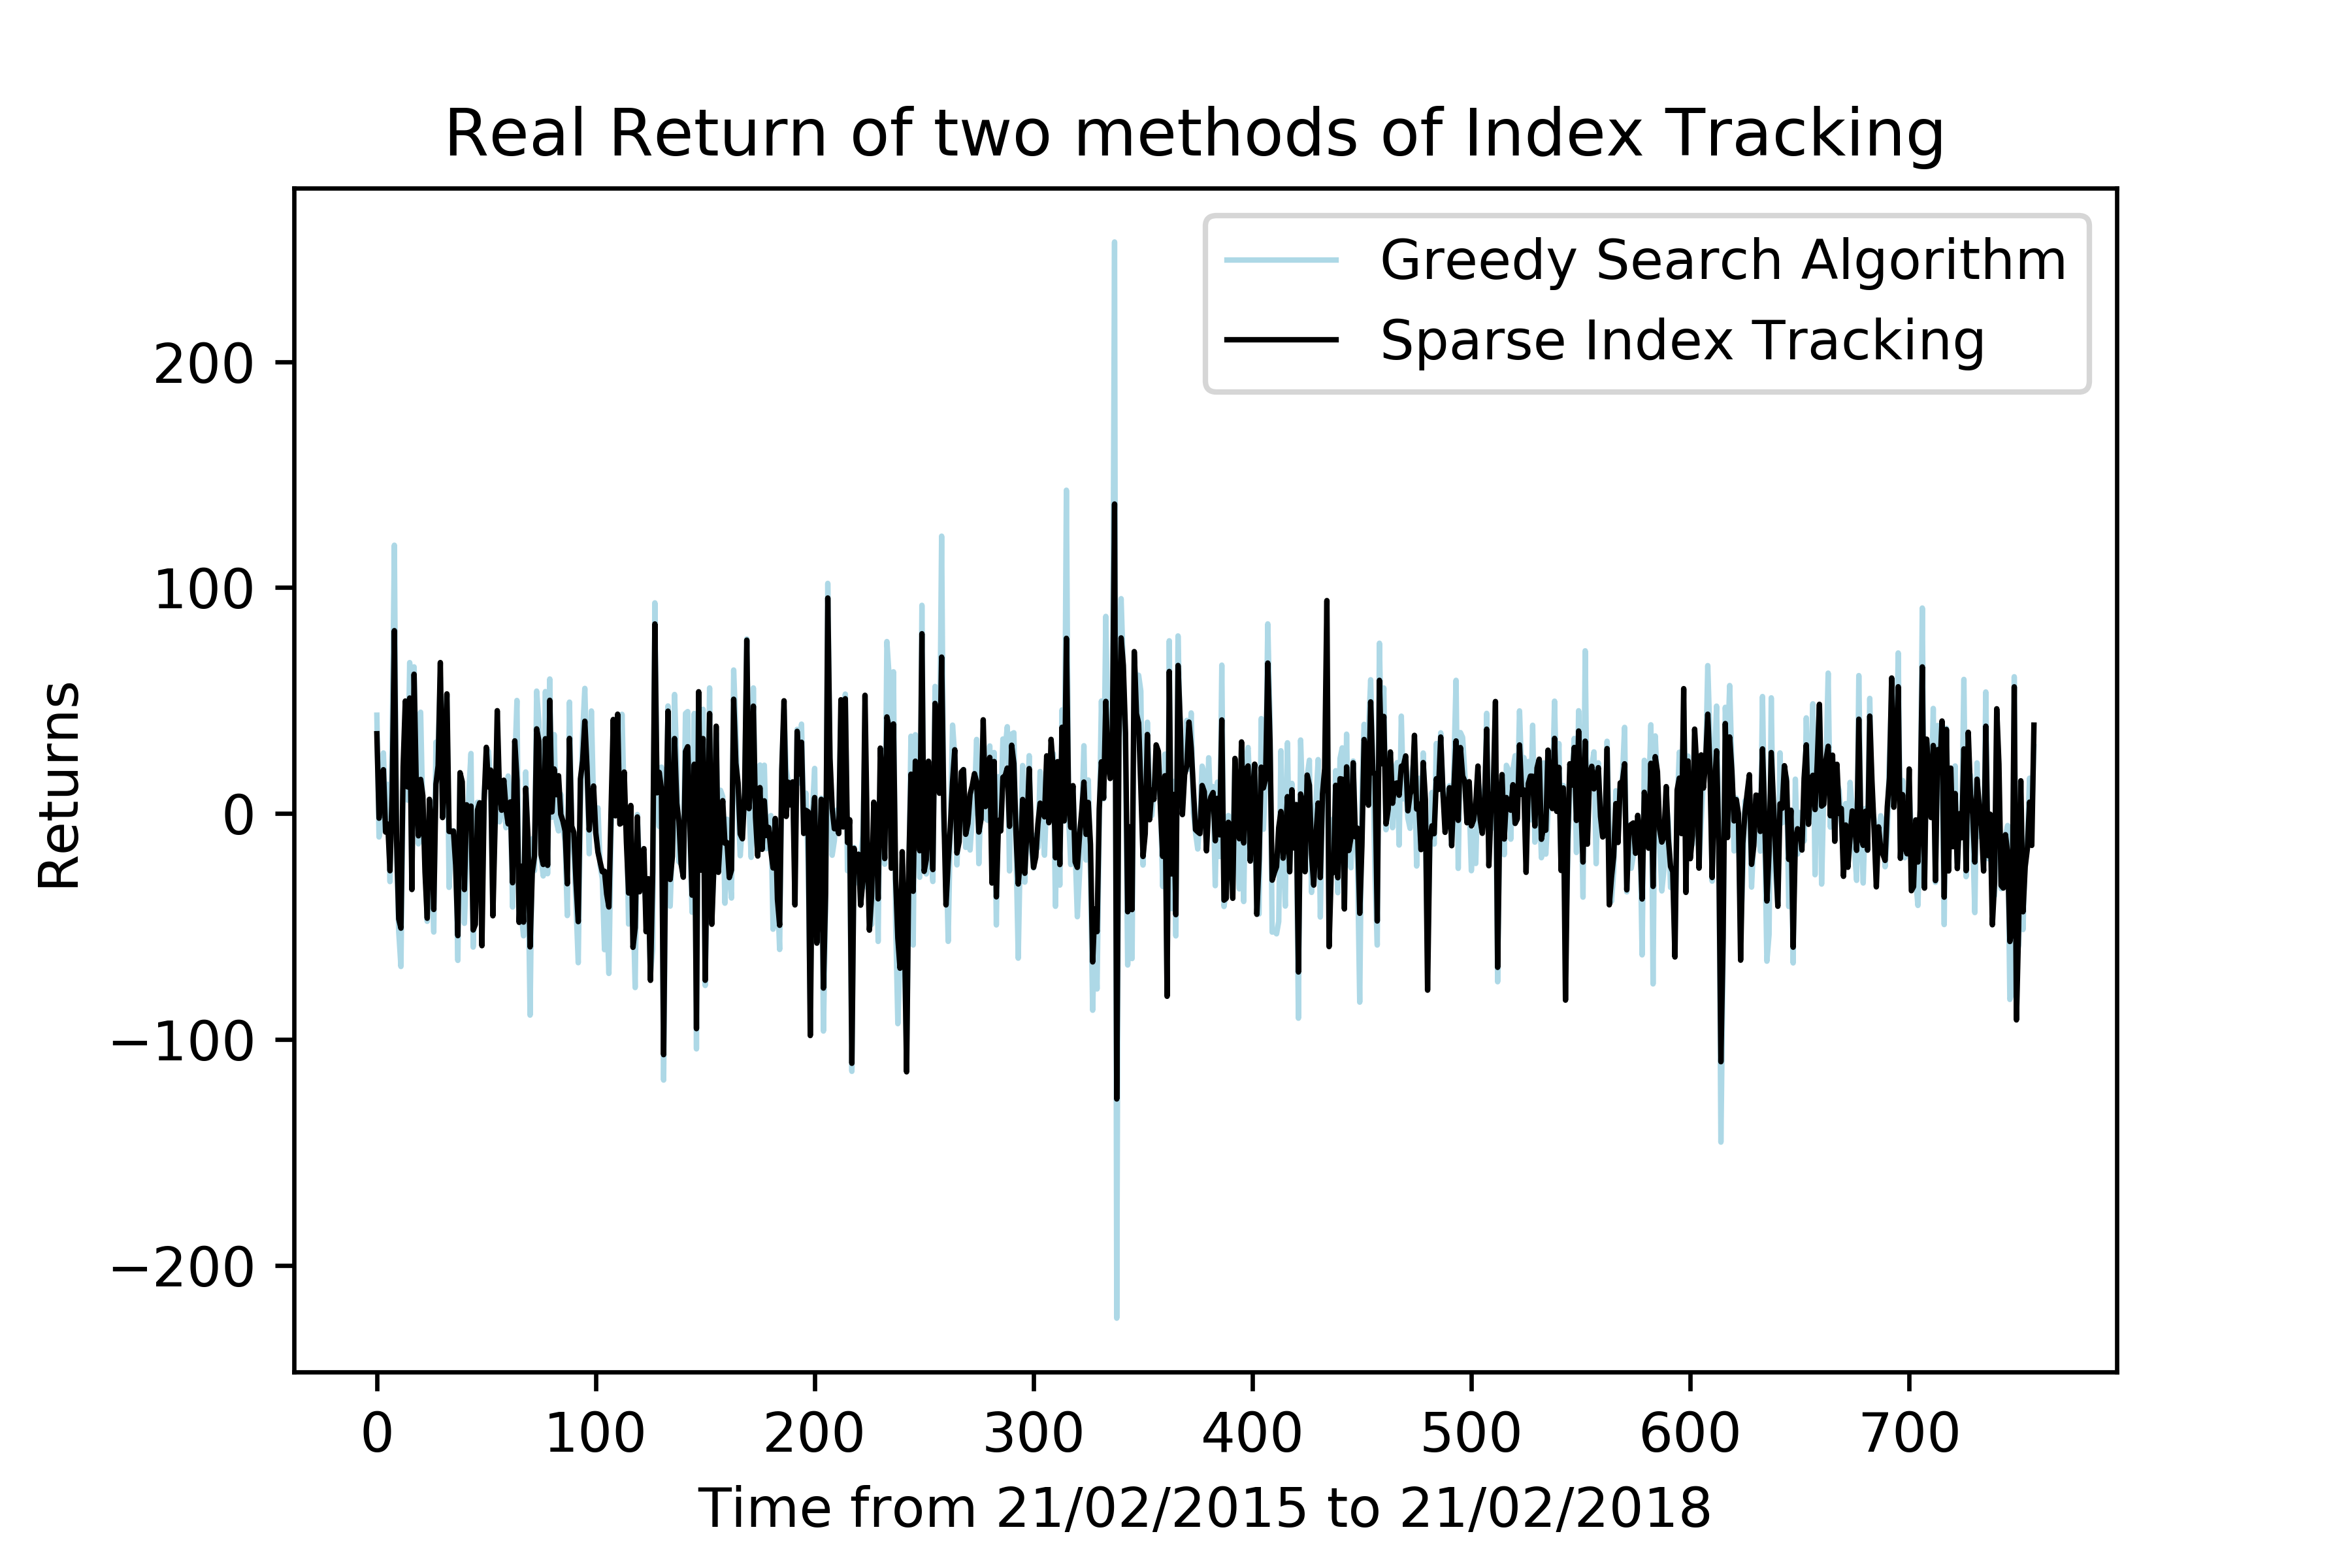
\includegraphics[width=0.5\textwidth]{11.png}
    \caption{\label{}Real Return of two index methods comparasion}
\end{figure}

%%%%%%%%%%%%%%%%%%%%%%%%%%%%%%%%%%%%%%%%%%%%%%%%%%%%%%%%%%%%%%%%%%%%%%%

\subsection{Question 7}

\begin{equation} \label{eq16}
\setlength{\abovedisplayskip}{3pt}
\setlength{\belowdisplayskip}{3pt}
\phi(x)=\sum_{i=1}^{n}\phi_{i}(x_{i})
\end{equation}

Transaction costs are used to the model number of costs, it could be represented as eq\eqref{eq16} by assuming transaction costs separately. $\phi$ is the transaction cost function for assets $i$ and $x$ is the vector of amounts transacted in each asset\cite{lobo2007portfolio}.

\begin{equation} \label{eq17}
\setlength{\abovedisplayskip}{3pt}
\setlength{\belowdisplayskip}{3pt}
\phi_{i}(x_{i})=\left\{\begin{matrix}
\alpha_{i}^{+}x_{i}\,, \qquad\ \ x_{i}\geqslant 0
\\ -\alpha_{i}^{-}x_{i}\,, \qquad x_{i}\leqslant 0
\end{matrix}\right.
\end{equation}

The simple model for the transaction can be modelled with 0 transaction cost function which is similar to the previous part. However, the portfolio with large linear transaction costs and convex constraints can be described by eq\eqref{eq17}. Thus, two convex linear equations can be calculated by a quadratic function. 

Consider there are N stocks, suppose the weights is $w=[w_{1},...,w_{n}]^{T}$, those weights can be adusted by $x=[x_{1},...,x_{n}]^{T}$, in addition, buying and selling can be controlled by positive and negative value of $x_{i}$, therefore, the transaction costs with changing weight can be represented as $(w+x)$. Moreover, suppose the return is $a=[a_{1},...a_{n}]$, the expected return $\overline{a}$ and covariance matrix $\Sigma$ is:

\begin{equation} \label{eq18}
\setlength{\abovedisplayskip}{3pt}
\setlength{\belowdisplayskip}{3pt}
\overline{a}=\bm{E}[A]\, , \quad \Sigma=\bm{E}(a-\overline{a})(a-\overline{a})^{T}
\end{equation}

By considering the riskless assets, the wealth is $\bm{W}=a^{T}(w+x)$ and the expected value and variance can be calculated by:

\begin{equation} \label{eq19}
\setlength{\abovedisplayskip}{3pt}
\setlength{\belowdisplayskip}{3pt}
\bm{EW}=\overline{a}^{T}(w+x)\, , \quad \bm{E(W-EW)^{2}}=(w+x)^{T}\Sigma(w+x)
\end{equation}

In addition, suppose the Budget constraint defined by $\bm{1}^{T}x+\phi(x)\leqslant0$ and the set of feasible potrfolios is $S$. The portfolio selection problem with transaction costs can be included in optimizing in this case as a objective function.

\begin{itemize}
\item maximizing expected \textbf{W} subject to constraint:

\begin{equation} \label{eq20}
\setlength{\abovedisplayskip}{3pt}
\setlength{\belowdisplayskip}{9pt}
maximize\ \overline{a}^{T}(w+x)\ subject\ to\ \bm{1}^{T} + \phi(x) \leqslant 0 \ and\ w+x \in S
\end{equation}

\item minimum smallest total cost subject to expected \textbf{W} with $r_{min}$ which is the desired lower bound:

\begin{equation} \label{eq21}
\setlength{\abovedisplayskip}{3pt}
\setlength{\belowdisplayskip}{9pt}
minimize\ \phi{(x)}\ subject\ to\ \overline{a}^{T}(w+x)\geqslant r_{min} \ and\ w+x \in S
\end{equation}

\end{itemize}

Budget constraint means the self-finance changing in the portfolio, it could limit the exposure to risk and prevent the money sink portfolio. The Budget constraint is defined in the previous part which is $\bm{1}^{T}x+\phi(x)\leqslant0$.

The short selling constraint sets a limit on how much short selling is permitted for each asset and it could be defined as imposeing a maximum of shortselling on asset $i$, $w_{i}+x_{i}\geqslant -s_{i}$.

The shortfall risk constraints mean to use different losses with acceptable probabilities to limit risk. It is a second order cone with inequality euclidean distance.

A specific problem discussed in section 1.6 of \cite{lobo2007portfolio} is:

\begin{equation} \label{eq22}
\setlength{\abovedisplayskip}{3pt}
\setlength{\belowdisplayskip}{9pt}
\begin{aligned}
&(27.1) \quad &maximize\quad \overline{a}^{T}(w+x^{+}-x^{-}) \\
&(27.2) \quad &subject\ to\ \bm{1}^{T}(x^{+}-x^{-})+\sum_{i=1}^{n}(\alpha_{i}^{+}x_{i}^{+}+\alpha_{i}^{-}x_{i}^{-})\leqslant0 \\
&(27.3) \quad &x_{i}^{+}\geqslant0, \quad x_{i}^{-}\geqslant0, \quad i=1,...,n \\
&(27.4) \quad &w_{i}+x_{i}^{+}-x_{i}^{-}\geqslant s_{i}, \quad x_{i}^{-}\geqslant0, \quad i=1,...,n\\
&(27.5) \quad &\Phi^{-1}(\eta_{j})\left \|\Sigma^{\frac{1}{2}}(w+x^{+}-x^{-})  \right \| \leqslant \overline{a}^{T}(w+x^{x}-x^{-})-\bm{W}_{j}^{low}, \quad j=1,2.
\end{aligned}
\end{equation}

According to eq\eqref{eq22}, it could find the objective function is $eq(27.1)$ and the constraints are linear transaction cost constraints $eq(27.2)$ and $eq(27.3)$, shortselling constraints $eq(27.4)$ and the shortfall risk constraints $eq(27.5)$.

In order to implement this in previous work, the CVX optimisation of the NaiveMV\_CVX can be changed to fit relevant constraints(adding and choosing variables in eq\eqref{eq22}). And for the Markowitz portfolio, the original parameters can be updated by $R=\overline{a}^{T}$ and $w=(w+x)$.

\begin{figure}[htbp]
    \centering
    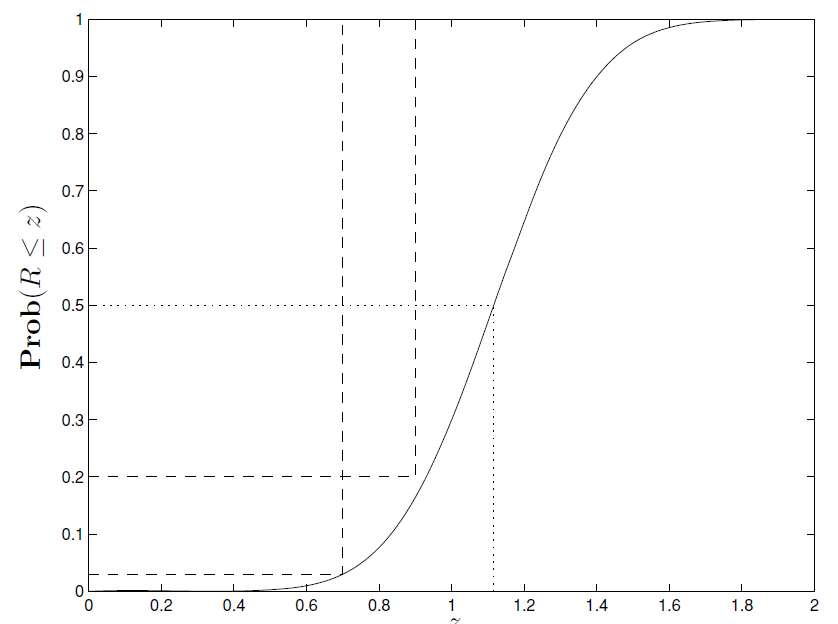
\includegraphics[width=0.5\textwidth]{12.png}
    \caption{\label{}Cumulative distribution function of the return\cite{lobo2007portfolio}}
\end{figure}

For 100 stocks with riskless assets, the cumulative distribution of the return is plotted in $Fig10$, it could find the expected return is corresponding to the 0.5 probability on the horizontal axis. In addition, two limits of constraints probability are shown in dashed lines, the $\eta$ and $\bm{W}$ can be chosen from the Fig2 which is:

\begin{equation} \label{eq23}
\setlength{\abovedisplayskip}{3pt}
\setlength{\belowdisplayskip}{9pt}
\eta_1=80\%, \quad \bm{W_{1}^{low}}=0.9; \quad and \quad \eta_2=97\%, \quad \bm{W_{2}^{low}}=0.7.
\end{equation}

%%%%%%%%%%%%%%%%%%%%%%%%%%%%%%%%%%%%%%%%%%%%%%%%%%%%%%%%%%%%%%%%%%%%%%%
\section{(B) 25 Marks}

An option provides the holder with the right to buy or sell a specified quantity of an underlying asset at a fixed price or before the expiration date of the option.

It can be defined by following notions:
\begin{itemize}
\item 
$K$: the strike price
\item
$S$: the value of the underlying asset
\item
$r$: the risk-free interest rate
\item
$T$: the time of maturity
\item
$t$: the current time
\item
$\mathcal{N}(x)$: the cummulative normal distribution
\item
$\sigma$: the standard deviation of the return of storck
\item
$V(S,t)$: the price of a derivative as function of time and stock price
\item
$C(S,t)$: the price of a European call option
\item
$P(S,t)$: the price of a European put option
\end{itemize}

Therefore, the Black-Scholes equation which is a partial differential equation can be defined by those notion:

\begin{equation} \label{eq24}
\setlength{\abovedisplayskip}{3pt}
\setlength{\belowdisplayskip}{9pt}
\frac{\partial{V}}{\partial{t}} + \frac{1}{2}\sigma^{2}S^{2} \frac{\partial^{2}V}{\partial{S}} + rS \frac{\partial{V}}{\partial{S}} - rV=0
\end{equation}

\subsection{Question 1}
\begin{itemize}
\item
$\mathcal{N}(x)$ is the standard normal cumulative distribution function and it represent as:

\begin{equation} \label{eq25}
\setlength{\abovedisplayskip}{3pt}
\setlength{\belowdisplayskip}{9pt}
\mathcal{N}(x)=\frac{1}{\sqrt{2\pi}} \int_{-\infty}^{x} e^{-\frac{z^2}{2}}\,\mathrm{d}z
\end{equation}

Therefore, the derivative of $\mathcal{N}(x)$ is:

\begin{equation} \label{eq26}
\setlength{\abovedisplayskip}{3pt}
\setlength{\belowdisplayskip}{9pt}
\mathcal{N'}(x)=\frac{1}{\sqrt{2\pi}} e^{-\frac{x^2}{2}} ~\\
\end{equation}


\item
Show that $S\mathcal{N'}(d_{1})=K\,exp(-r(T-t))\mathcal{N'}(d_{2})$ where $d_{1}$ and $d_{2}$ were defined as:

\begin{equation} \label{eq27}
\setlength{\abovedisplayskip}{3pt}
\setlength{\belowdisplayskip}{3pt}
d_{1}=\frac{log(\frac{S}{K})+(r+\frac{\sigma^{2}}{2})(T-t)}{\sigma \sqrt{(T-t)}}
\end{equation}

\begin{equation} \label{eq28}
\setlength{\abovedisplayskip}{3pt}
\setlength{\belowdisplayskip}{9pt}
d_{2}= d_{1} - \sigma \sqrt{(T-t)}
\end{equation}

Substitute $d_{1}$ and $d_{2}$ into eq\eqref{eq26}:

\begin{equation} \label{eq29}
\setlength{\abovedisplayskip}{3pt}
\setlength{\belowdisplayskip}{9pt}
\mathcal{N'}{(d_{1})} = e^{\frac{-d_{1}^{2}}{2}}
\end{equation}

\begin{equation} \label{eq30}
\setlength{\abovedisplayskip}{3pt}
\setlength{\belowdisplayskip}{9pt}
\mathcal{N'}{(d_{2})} = e^{\frac{-d_{2}^{2}}{2}}=e^{\frac{-d_{1}^{2}}{2}}+ d_{1}\sigma \sqrt{(T-t)}-\frac{\sigma^{2}(T-t)}{2}
\end{equation}

and then take log on both sides of proved equation and substitude eq\eqref{eq29} and eq\eqref{eq30}:

\begin{equation} \label{eq31}
\setlength{\abovedisplayskip}{3pt}
\setlength{\belowdisplayskip}{9pt}
log(S\mathcal{N'}(d_{1})) = log(S) - \frac{d_{1}^{2}}{2}
\end{equation}

\begin{equation} \label{eq32}
\setlength{\abovedisplayskip}{3pt}
\setlength{\belowdisplayskip}{9pt}
log(K\, exp(-r(T-t)\mathcal{N'}(d_{2})) = log(K)-\frac{-d_{1}^{2}}{2} + d_{1}\sigma \sqrt{(T-t)} -(r+\frac{\sigma^{2}}{2})(T-t)
\end{equation}

Finally, substitude eq\eqref{eq27} and eq\eqref{eq28} into the difference value of eq\eqref{eq31} and eq\eqref{eq32}:

\begin{equation} \label{eq33}
\setlength{\abovedisplayskip}{3pt}
\setlength{\belowdisplayskip}{9pt}
log(\frac{S}{K})-\frac{log(\frac{S}{K})+(r+\frac{\sigma^{2}}{2})(T-t)}{\sigma \sqrt{(T-t)}} \sigma \sqrt{(T-t)} - (r+\frac{\sigma^{2}}{2})(T-t) = 0
\end{equation}

Therefore, $S\mathcal{N'}(d_{1})=K\,exp(-r(T-t))\mathcal{N'}(d_{2})$ proved. ~\\

\item
Calculate the derivaties $\frac{\partial{d_{1}}}{\partial{S}}$ and $\frac{\partial{d_{2}}}{\partial{S}}$.

Those two expressions are equivalent because of $\frac{\partial{d_{1}}}{\partial{d_{2}}}=1$.

\begin{equation} \label{eq34}
\setlength{\abovedisplayskip}{3pt}
\setlength{\belowdisplayskip}{9pt}
\frac{\partial{d_{1}}}{\partial{S}} = \frac{\partial{d_{2}}}{\partial{S}} = \frac{\partial{d_{1}}}{\partial{S}} \frac{\partial{d_{2}}}{\partial{d_{1}}} = \frac{1}{S\sigma \sqrt{(T-t)}} ~\\
\end{equation}

\item

With the solution for the call option price given by:

\begin{equation} \label{eq35}
\setlength{\abovedisplayskip}{3pt}
\setlength{\belowdisplayskip}{9pt}
c = S\mathcal{N'}(d_{1})-K\,exp(-r(T-t))\mathcal{N'}(d_{2})
\end{equation}

show that its derivative with repect to time is:

\begin{equation} \label{eq36}
\setlength{\abovedisplayskip}{3pt}
\setlength{\belowdisplayskip}{9pt}
\frac{\partial{c}}{\partial{t}} = -rK\, exp(-r(T-t)) \mathcal{N}(d_{2}) - S\mathcal{N'}(d_{1}) \frac{\sigma}{2\sqrt{(T-t)}}
\end{equation}

Directly apply derivative on eq\eqref{eq35}:

\begin{equation} \label{eq37}
\setlength{\abovedisplayskip}{3pt}
\setlength{\belowdisplayskip}{9pt}
\frac{\partial{c}}{\partial{t}} = S\mathcal{N'}(d_{1}) \frac{\partial{d_{1}}}{\partial{t}} - rKe^{(-r(T-t))} \mathcal{N}(d_{2}) - Ke^{(-r(T-t))}\mathcal{N'}(d_{2})\frac{\partial{d_{2}}}{\partial{t}}
\end{equation}

Substitude previous equation $S\mathcal{N'}(d_{1})=K\,exp(-r(T-t))\mathcal{N'}(d_{2})$ to cancel terms:

\begin{equation} \label{eq38}
\setlength{\abovedisplayskip}{3pt}
\setlength{\belowdisplayskip}{9pt}
eq\eqref{eq37} = - rKe^{(-r(T-t))} \mathcal{N}(d_{2}) + S\mathcal{N'}(d_{1}) (\frac{\partial{d_{1}}}{\partial{t}} - \frac{\partial{d_{2}}}{\partial{t}}) = eq\eqref{eq36}
\end{equation}

\item

Show that $\frac{\partial{c}}{\partial{S}} = \mathcal{N}(d_{1})$.

Directly apply derivative with $S\mathcal{N'}(d_{1})=K\,exp(-r(T-t))\mathcal{N'}(d_{2})$ to cancel terms and conclusion in eq\eqref{eq34}:

\begin{equation} \label{eq39}
\setlength{\abovedisplayskip}{3pt}
\setlength{\belowdisplayskip}{9pt}
\frac{\partial{c}}{\partial{S}} = \mathcal{N}(d_{1}) + S\mathcal{N'}(d_{1})(\frac{\partial{d_{1}}}{\partial{S}} - \frac{\partial{d_{2}}}{\partial{S}}) = \mathcal{N}(d_{1})
\end{equation}

\item

Differentiating eq\eqref{eq39} again to get:

\begin{equation} \label{eq40}
\setlength{\abovedisplayskip}{3pt}
\setlength{\belowdisplayskip}{9pt}
\frac{\partial^{2}{c}}{\partial{S}^{2}} = \mathcal{N'}(d_{1}) \frac{1}{S\sigma \sqrt{(T-t)}}
\end{equation}

The Black-Scholes models is defined at the beginning of this part which is eq\eqref{eq24}, for the call option, the price of a derivative $V$ is instead of the price of European call option $C$. Then substitude previous conclusions into this model:

\begin{equation} \label{eq41}
\setlength{\abovedisplayskip}{3pt}
\setlength{\belowdisplayskip}{9pt}
\begin{split}
eq\eqref{eq24} = - rKe^{(-r(T-t))} \mathcal{N}(d_{2}) - S\mathcal{N'}(d_{1})(\frac{\sigma}{2 \sqrt{(T-t)}}) \\
 + rS\mathcal{N}(d_{1}) + \frac{1}{2}\sigma^{2}S^{2} \frac{\mathcal{N'}(d_{1})}{\sigma S \sqrt{(T-t)}} -rc \\
= r(-Ke^{-r(T-t)})\mathcal{N}{d_{2}} + S\mathcal{N}{d_{1}}-c)=0
\end{split}
\end{equation}

Thus, the call option in Black-Scholes models can be derived:

\begin{equation} \label{eq42}
\setlength{\abovedisplayskip}{3pt}
\setlength{\belowdisplayskip}{9pt}
c = S\mathcal{N}{(d_{1})} - Ke^{(-r(T-t))} \mathcal{N}(d_{2})
\end{equation}

\end{itemize}

%%%%%%%%%%%%%%%%%%%%%%%%%%%%%%%%%%%%%%%%%%%%%%%%%%%%%%%%%%%%%%%%%%%%%%%

\subsection{Question 2}


Evaluate the option prices of FTSE100 index during February to December 1994 by the Black-Scholes model.

The formula of the call option in Black-Scholes was defined at previous eq\eqref{eq42}, similarly, the put option can be derived in a same procedure which is:

\begin{equation} \label{eq43}
\setlength{\abovedisplayskip}{3pt}
\setlength{\belowdisplayskip}{9pt}
p = Ke^{(-r(T-t))} \mathcal{N}(d_{-2}) - S\mathcal{N}{(d_{-1})}
\end{equation}

Suppose the value of the market variable at the end of day $i$ is $S_{i}$, the volatility of stocks can be deifned as eq\eqref{eq44} and eq\eqref{eq45} which come from secton 22.1 in \cite{hull2016options}.

\begin{equation} \label{eq44}
\setlength{\abovedisplayskip}{3pt}
\setlength{\belowdisplayskip}{9pt}
\mu_{i} = ln\frac{S_{i}}{S_{i-1}}
\end{equation}

\begin{equation} \label{eq45}
\setlength{\abovedisplayskip}{3pt}
\setlength{\belowdisplayskip}{9pt}
\sigma_{n} = \sqrt{\frac{1}{m-1}\sum{_{i=1}^{m}(\mu_{n-i}-\overline{\mu})^{2}}}
\end{equation}

And the last three fourths data's estimated historical volatilities $\overline{\sigma}$ can be calculated by $\overline{\sigma}=\frac{\sigma}{\sqrt{\uptau}}$ in a sliding window of range $t-\frac{T}{4}$. According to above equation, the calculated volatilities are shown in $Fig11$.

\begin{figure}[htbp]
    \centering
    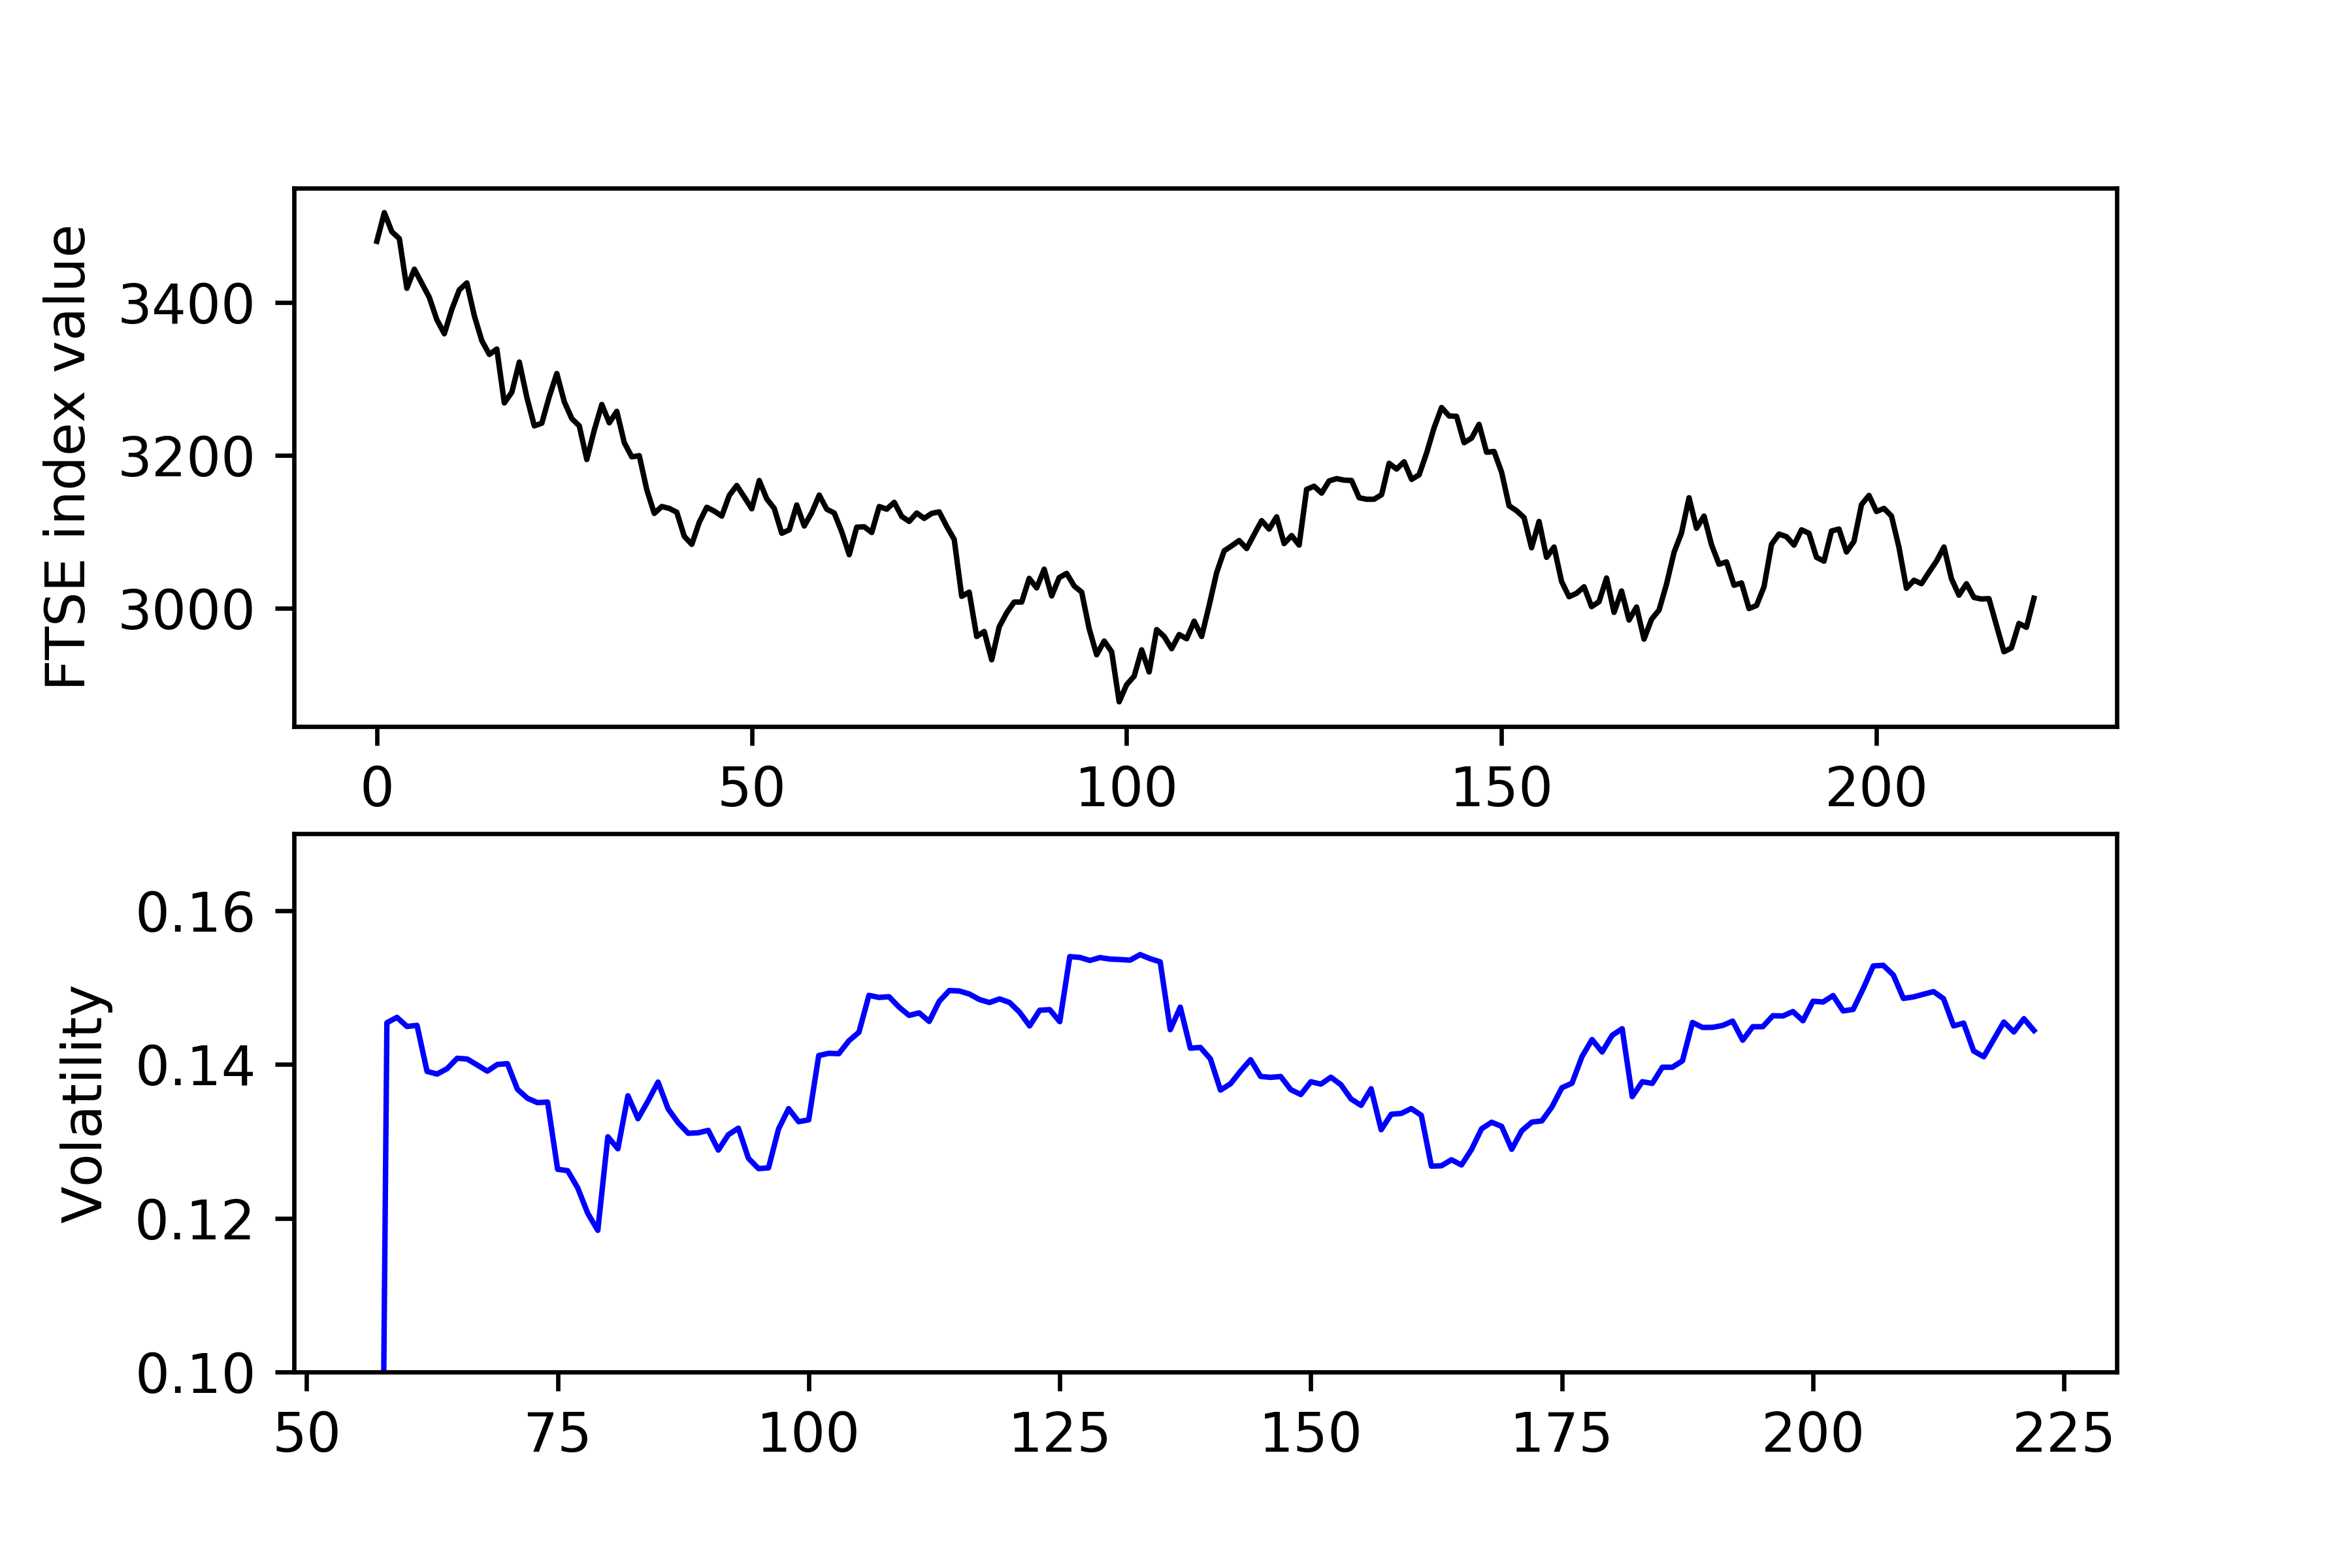
\includegraphics[width=0.5\textwidth]{13.png}
    \caption{\label{}assets value and historical volatility of 10 files}
\end{figure}

The annumal interst rate during the period $T$ is 6\%. Therefore, the call and put option price can be obtained by eq\eqref{eq42} and eq\eqref{eq43}.

\begin{figure}[htbp]
    \centering
    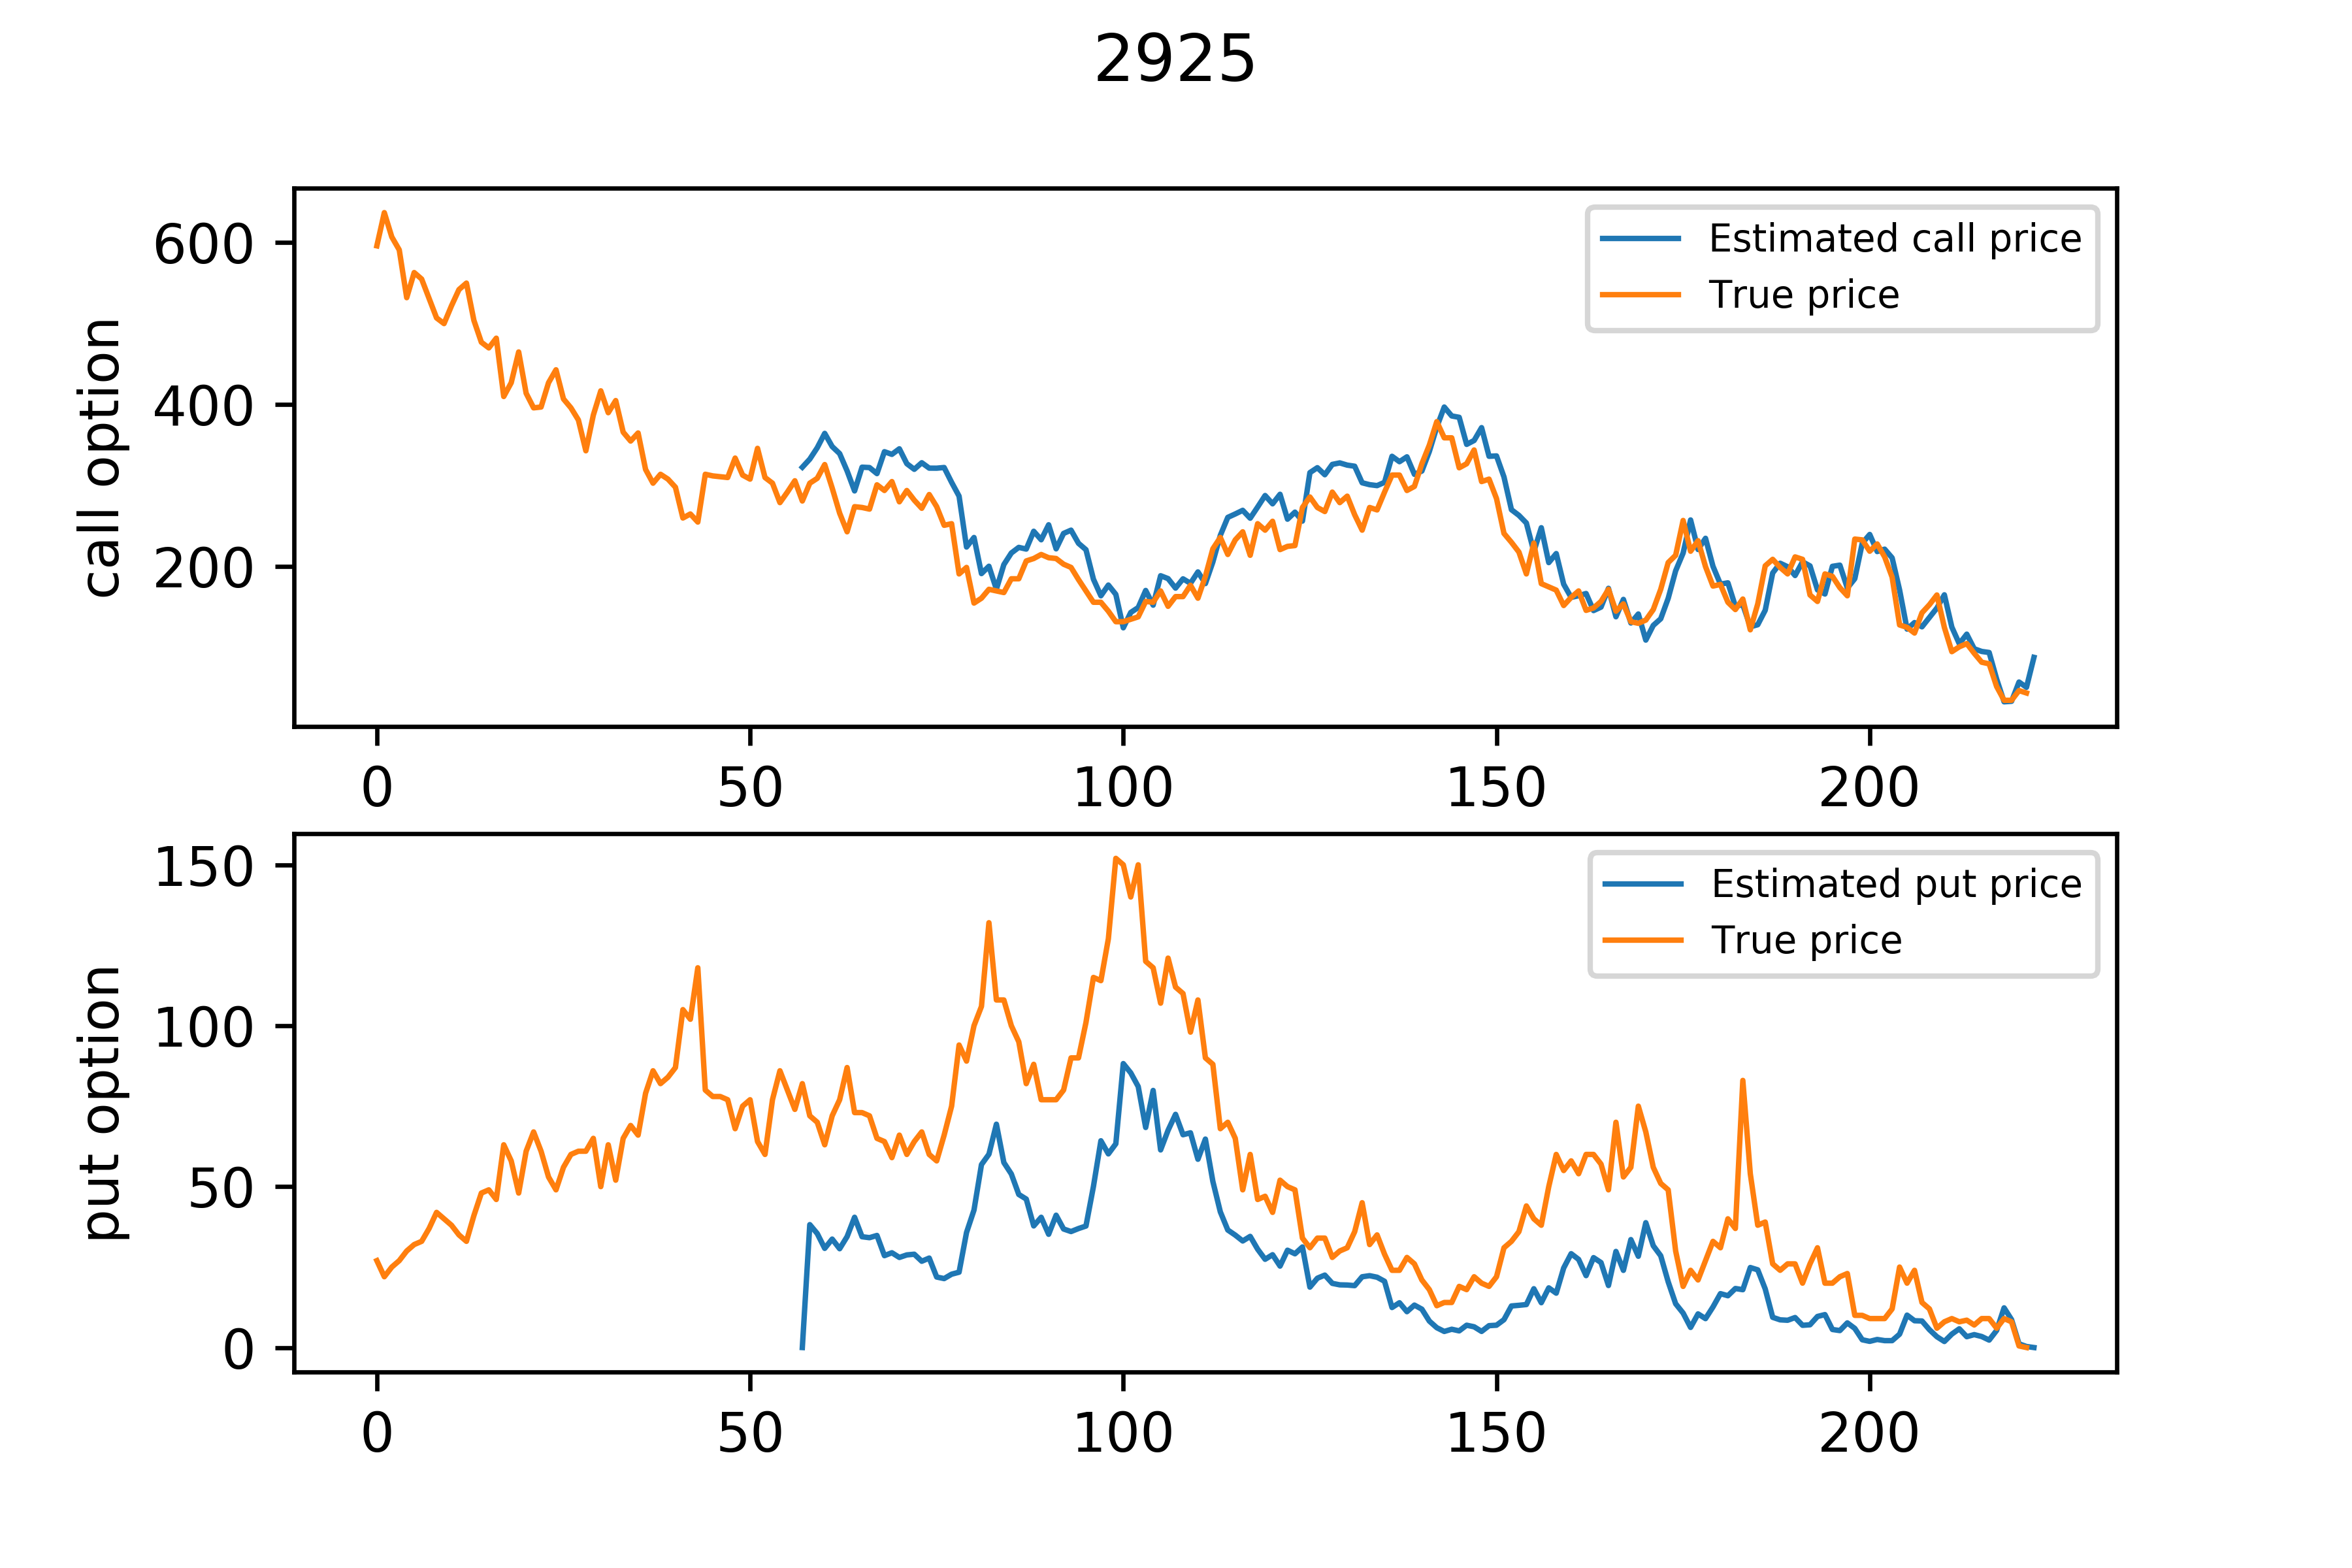
\includegraphics[width=0.5\textwidth]{14.png}
    \caption{\label{}$\overline{diff\_call}=-19.4848$, $\overline{diff\_put}=27.0937$}
\end{figure}

\begin{figure}[htbp]
    \centering
    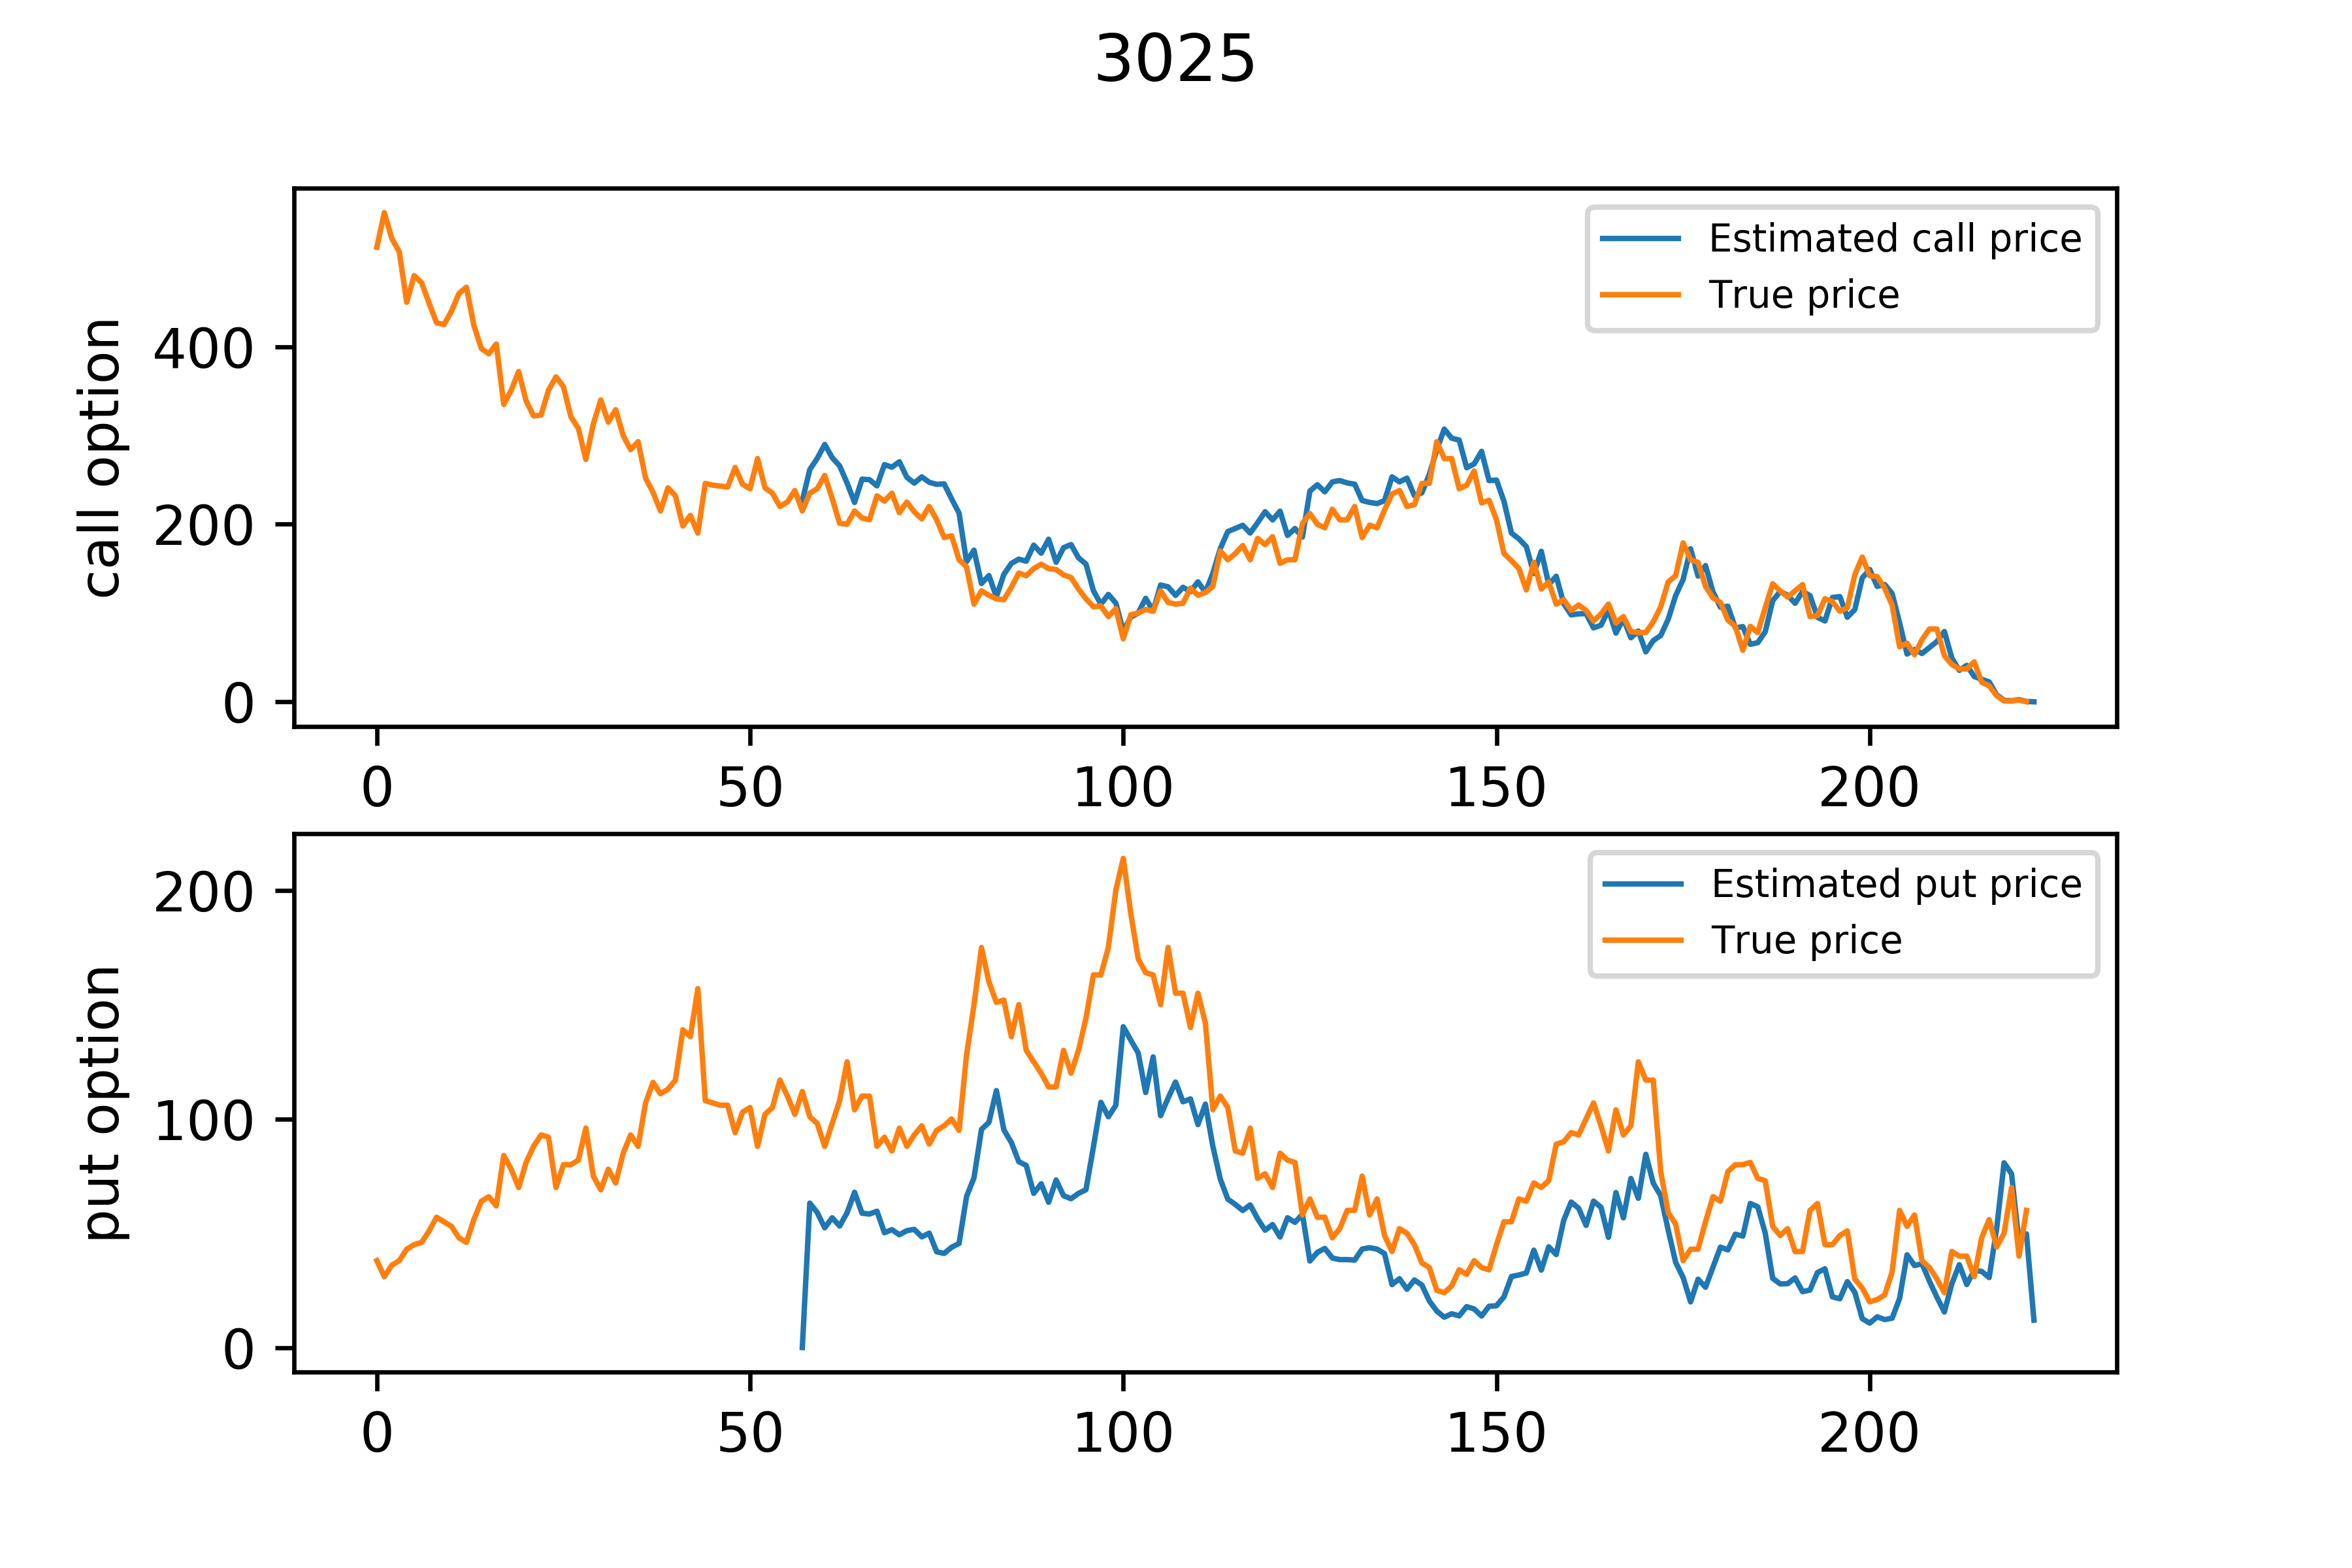
\includegraphics[width=0.5\textwidth]{15.png}
    \caption{\label{}$\overline{diff\_call}=-12.2427$, $\overline{diff\_put}=31.8830$}
\end{figure}

\begin{figure}[htbp]
    \centering
    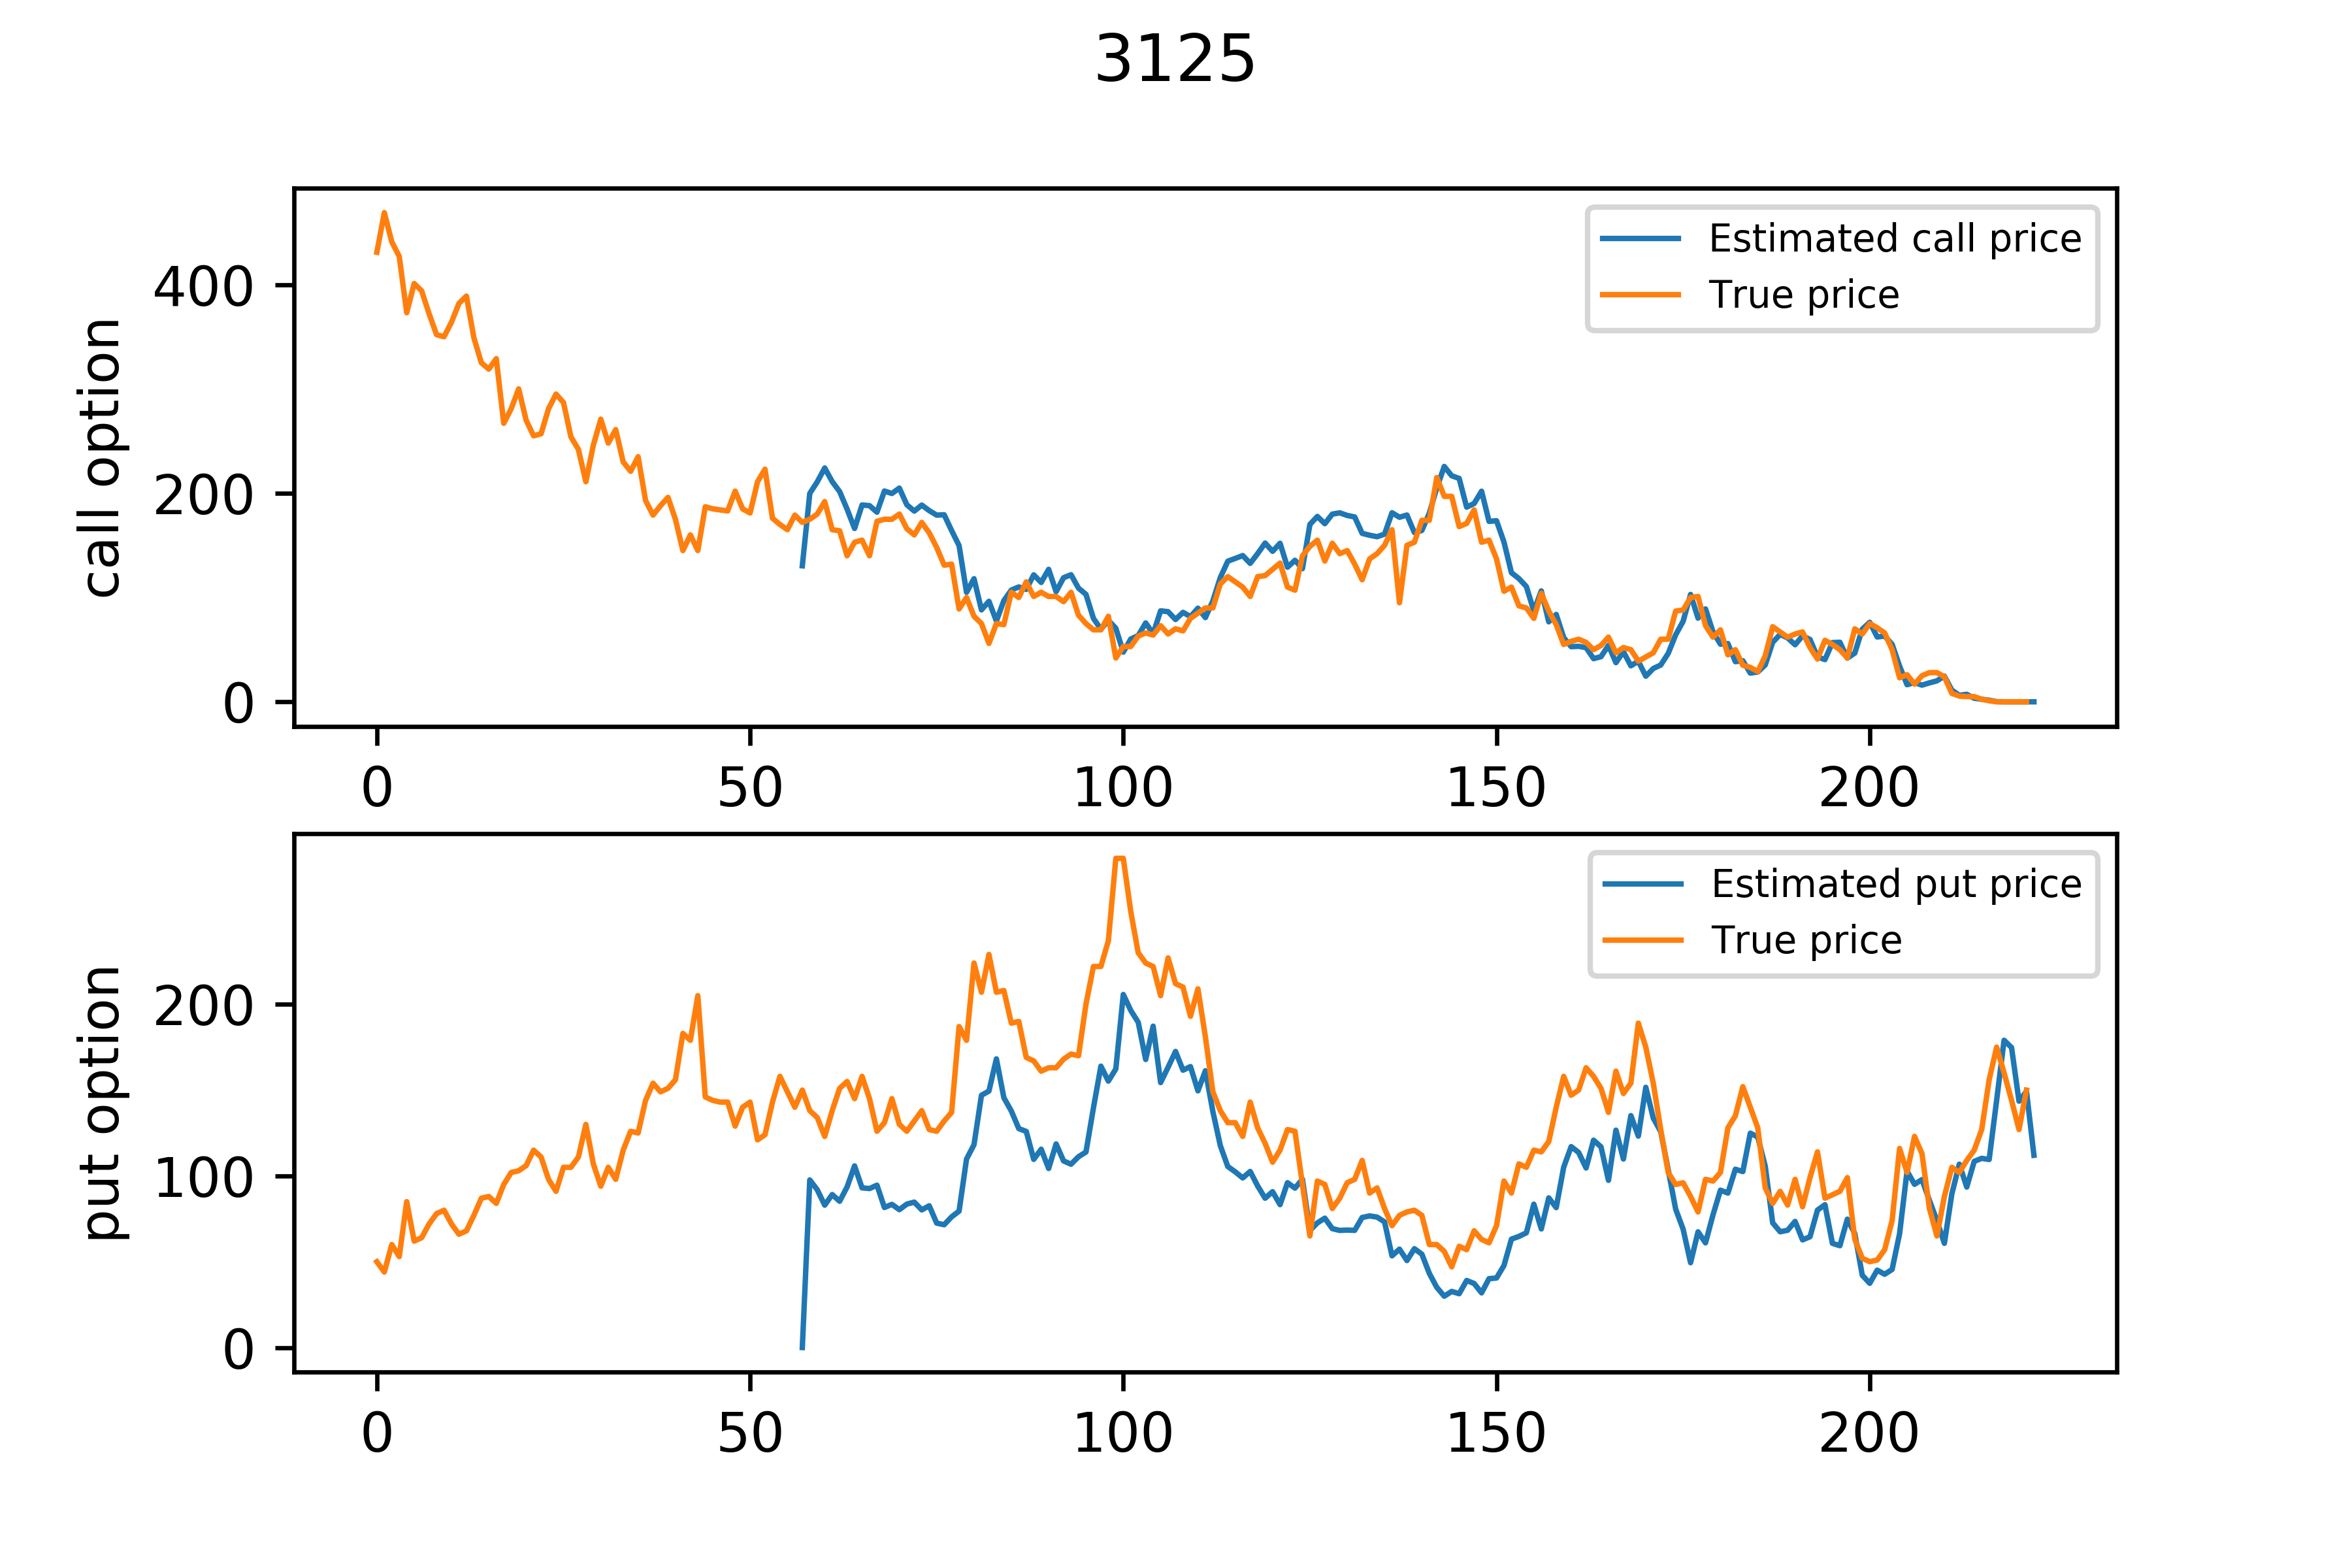
\includegraphics[width=0.5\textwidth]{16.png}
    \caption{\label{}$\overline{diff\_call}=-9.4576$, $\overline{diff\_put}=34.5226$}
\end{figure}

\begin{figure}[htbp]
    \centering
    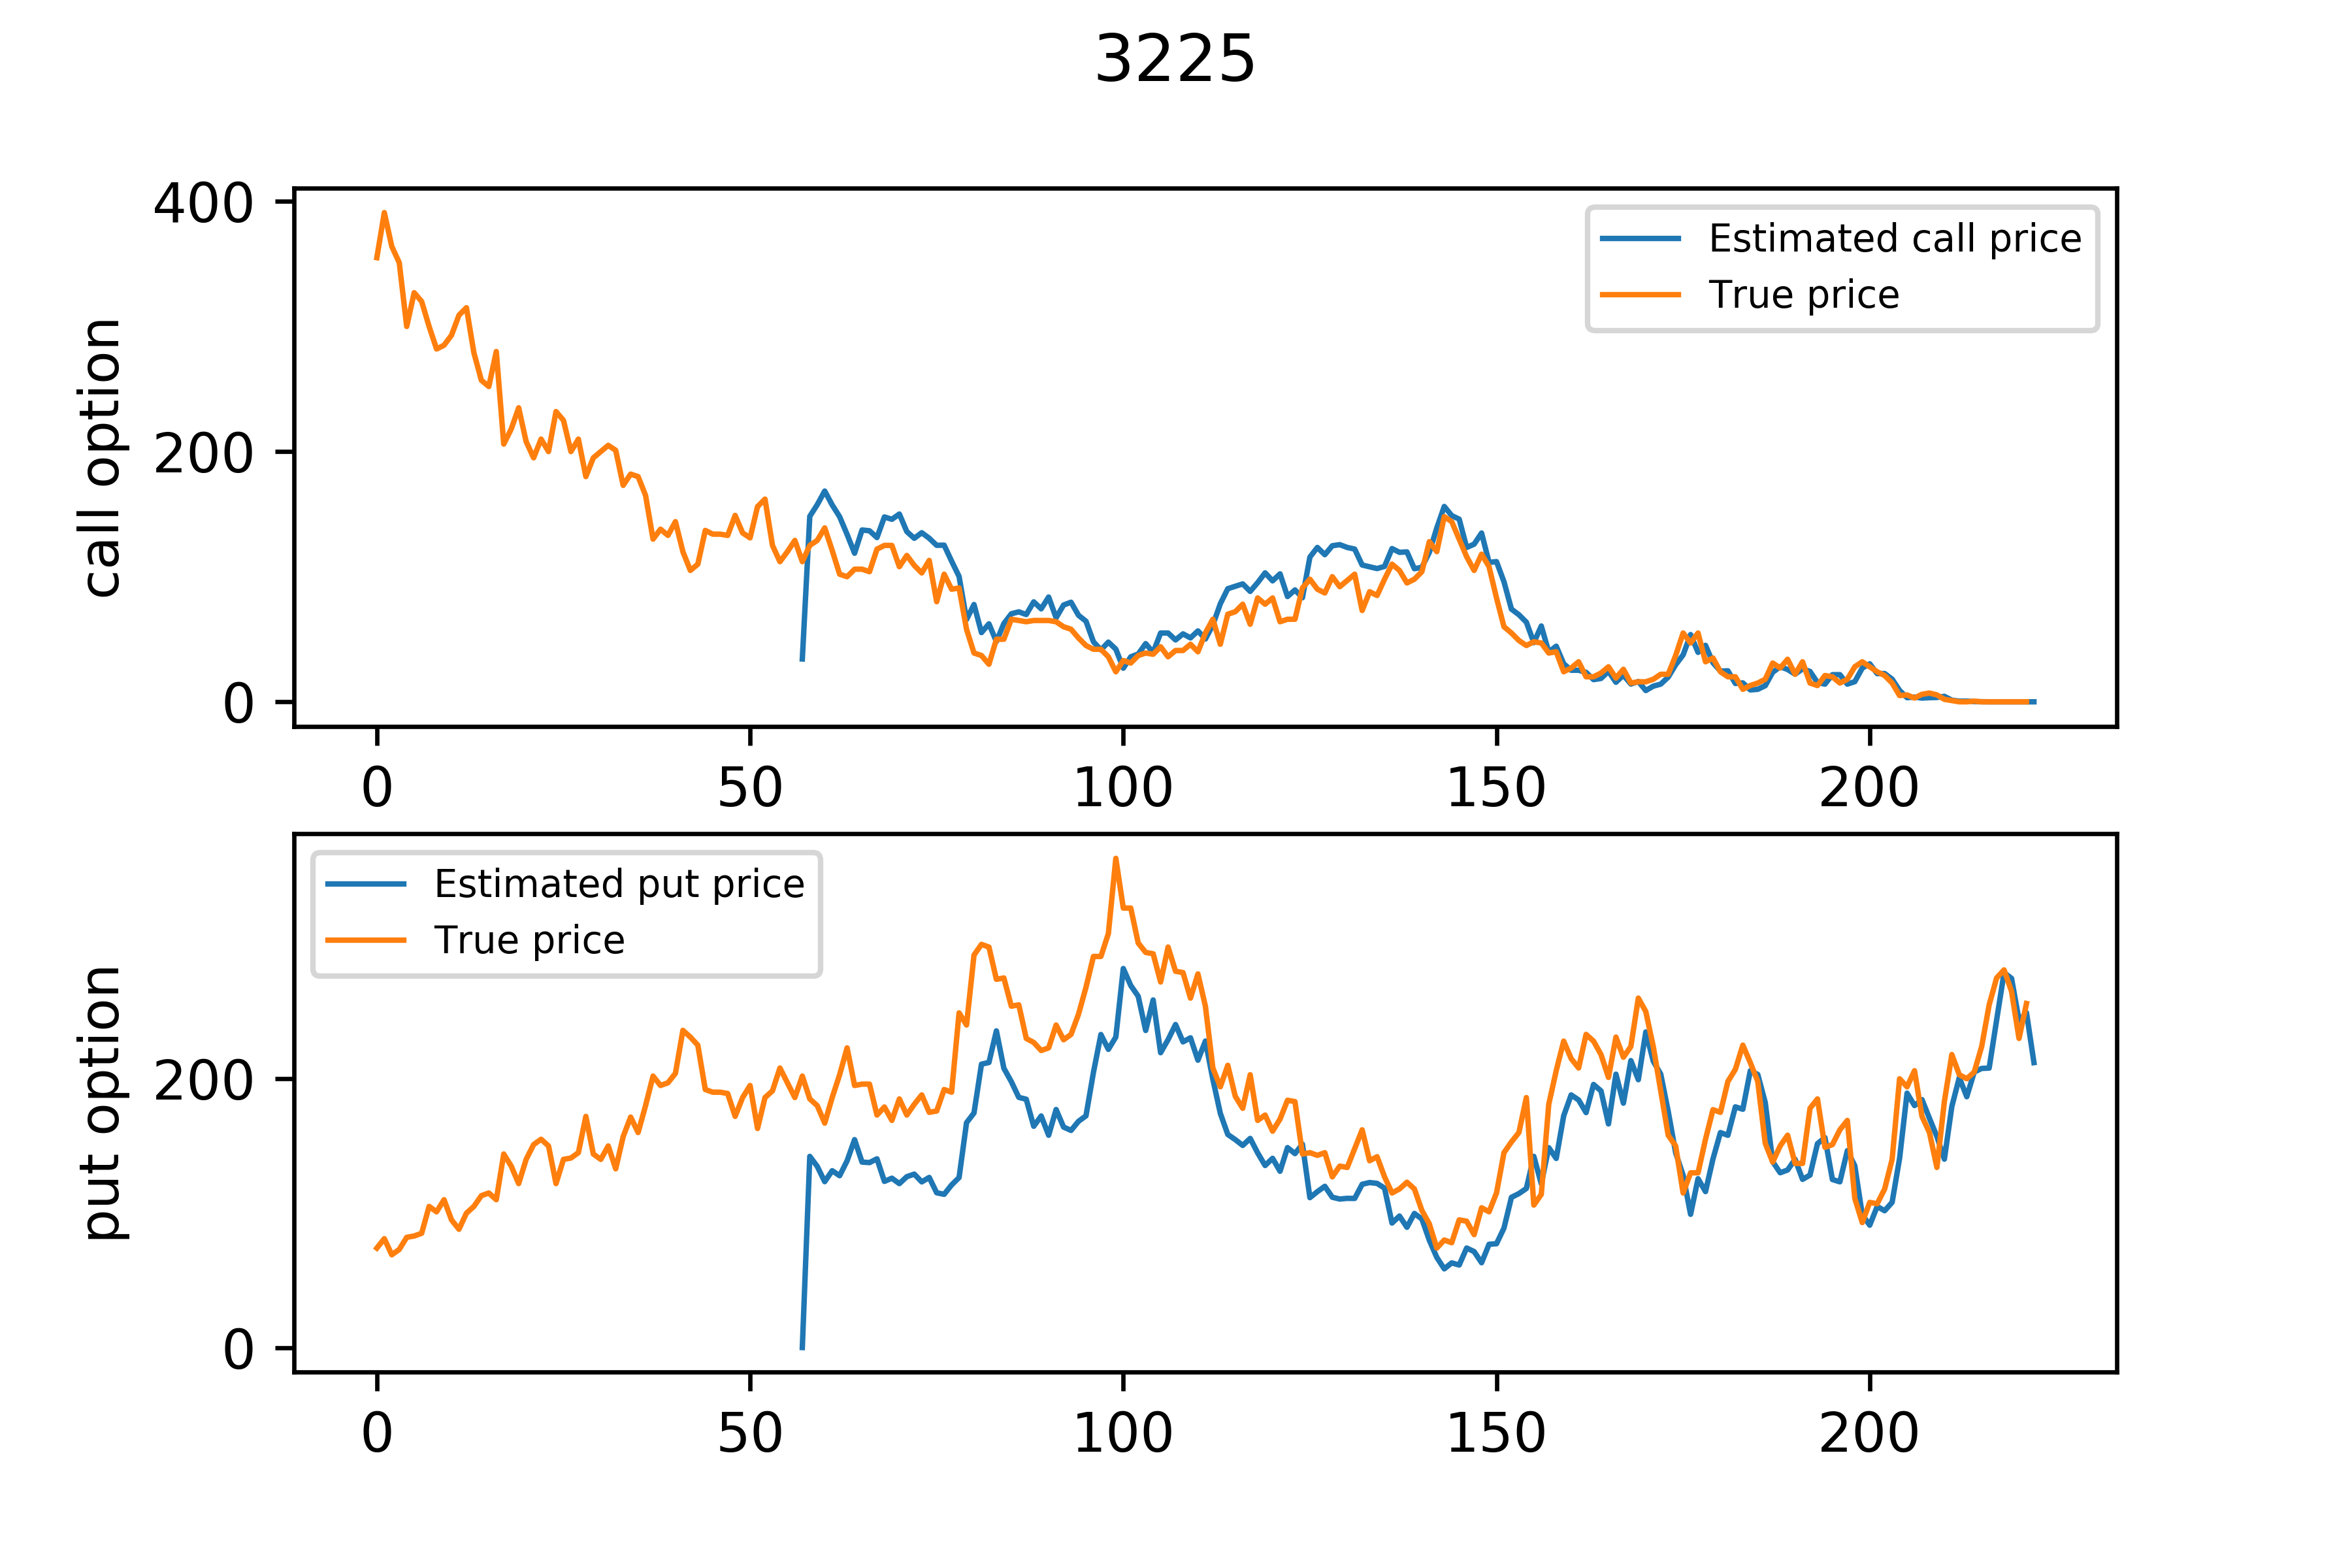
\includegraphics[width=0.5\textwidth]{17.png}
    \caption{\label{}$\overline{diff\_call}=-8.5385$, $\overline{diff\_put}=35.1544$}
\end{figure}

\begin{figure}[htbp]
    \centering
    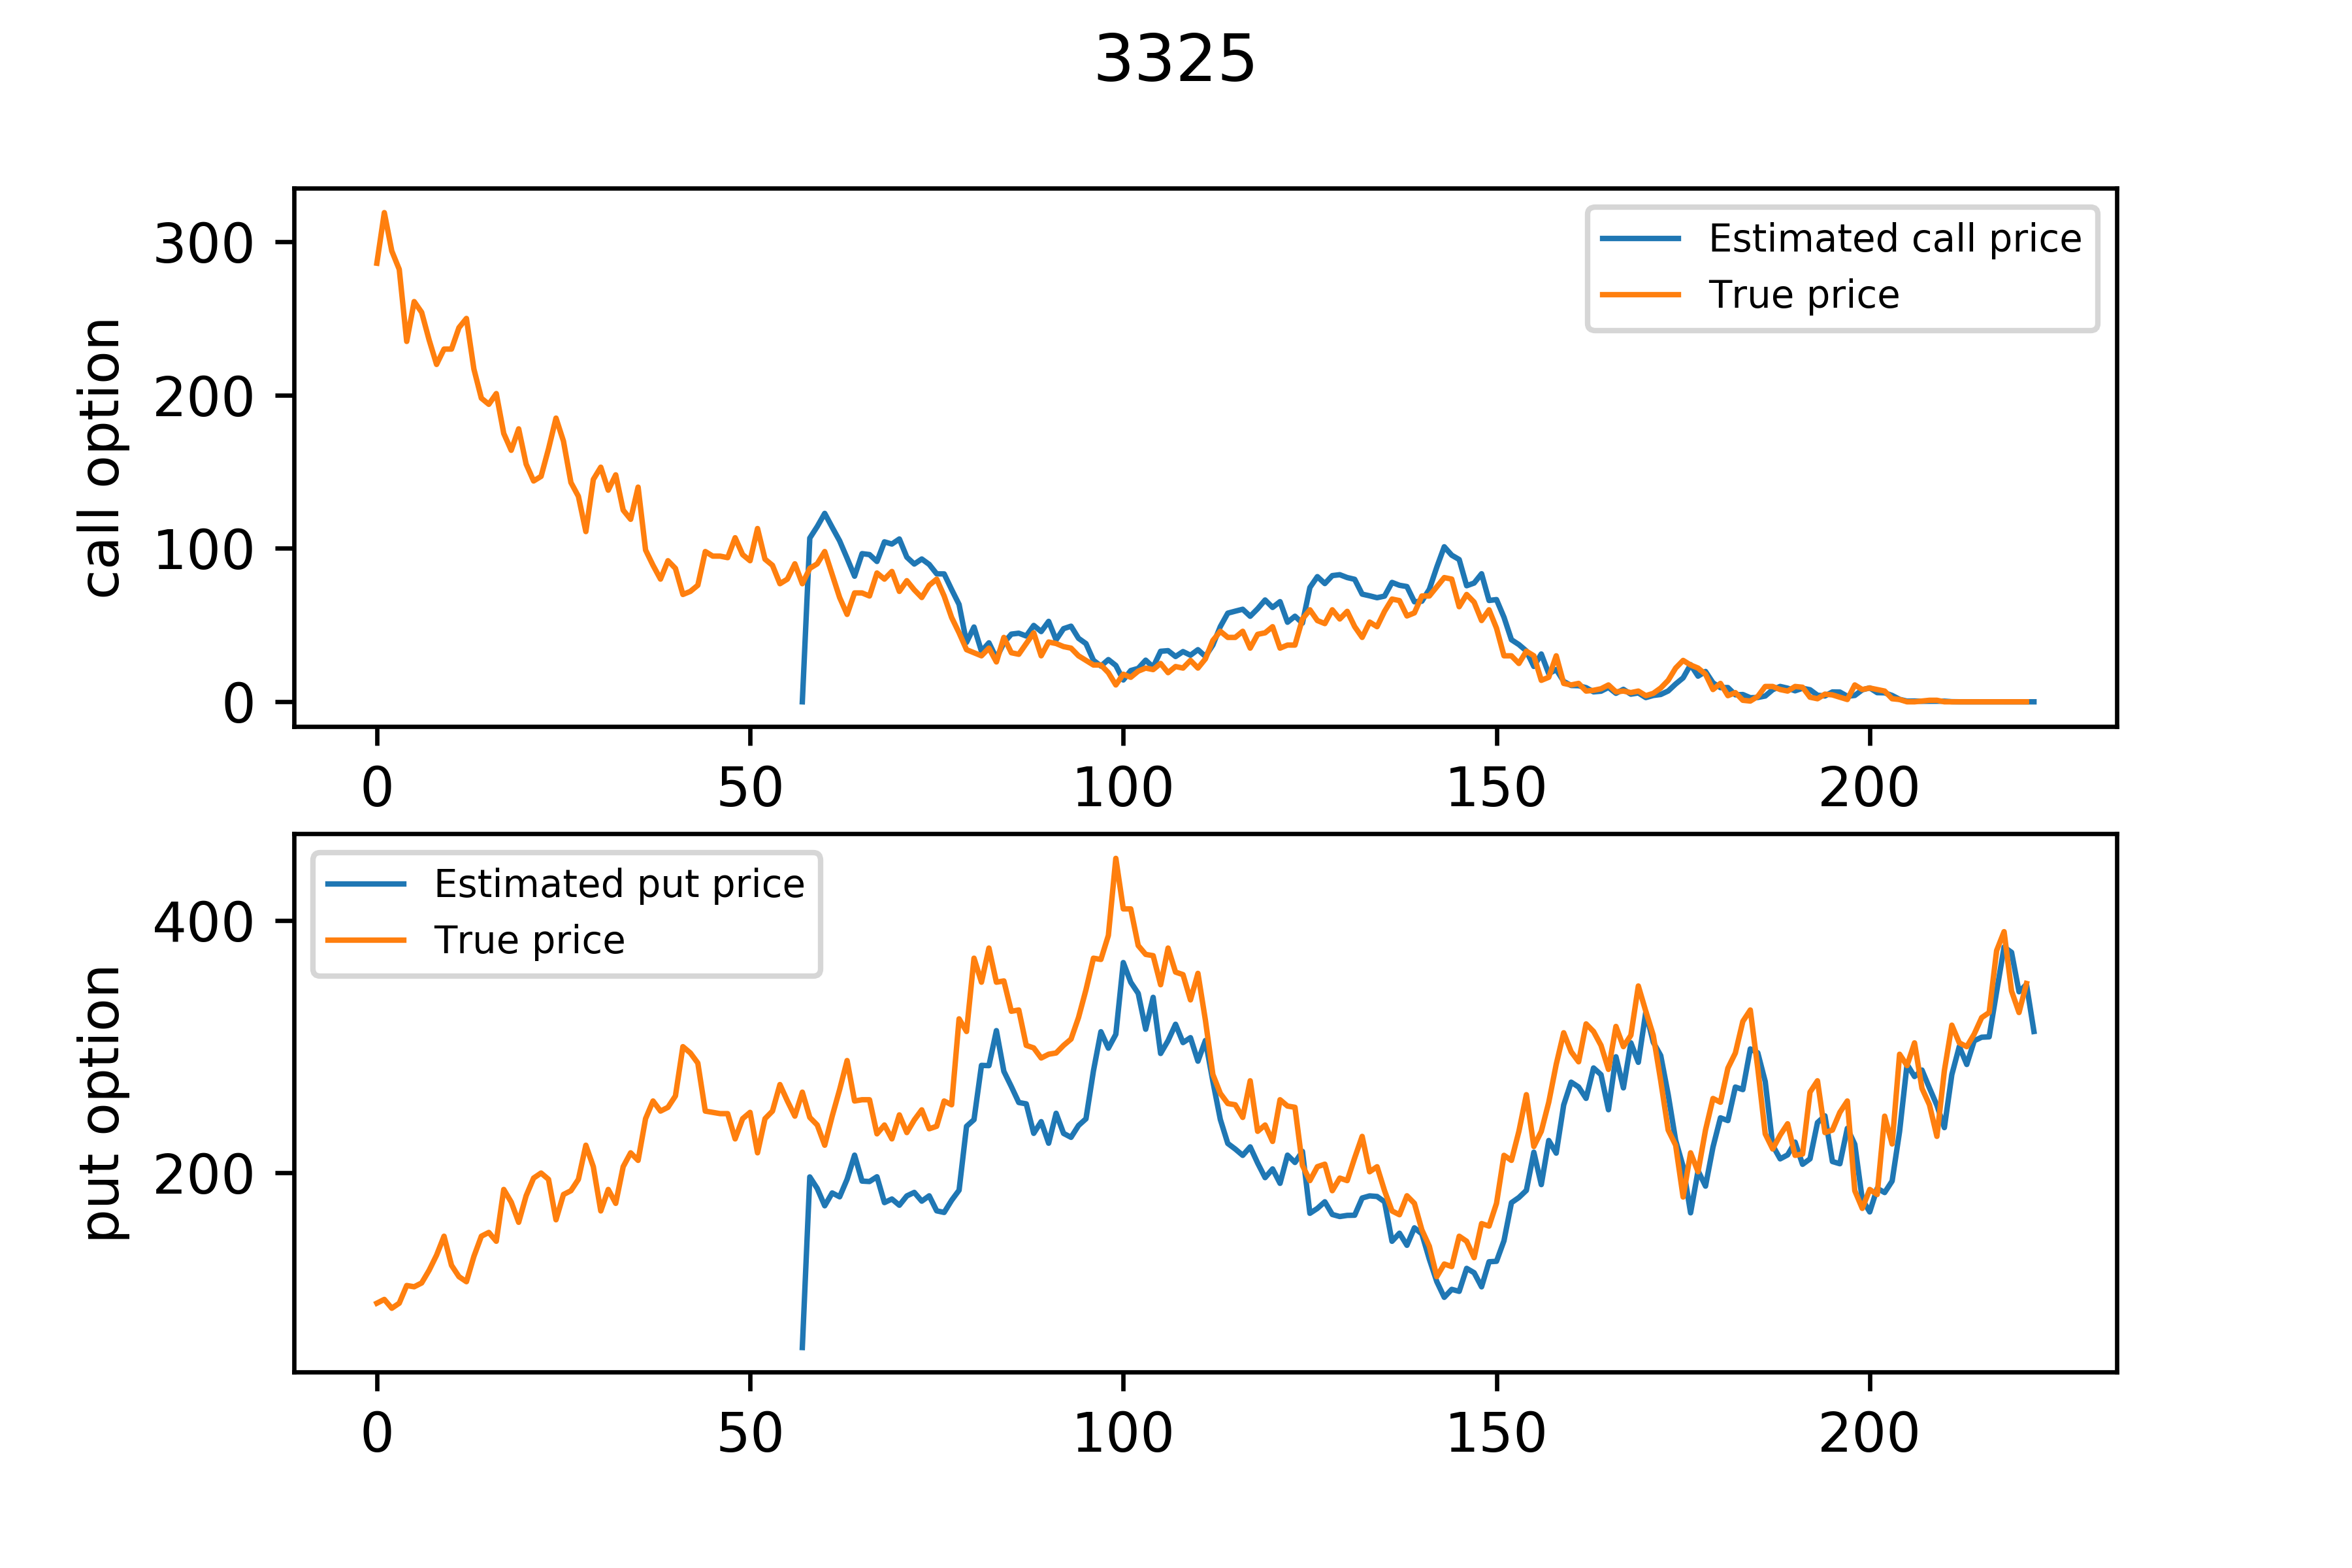
\includegraphics[width=0.5\textwidth]{18.png}
    \caption{\label{}$\overline{diff\_call}=-6.9645$, $\overline{diff\_put}=36.6791$}
\end{figure}

$Fig12$ to $Fig16$ are comparison diagram of computed call\/put prices with original value, the mean difference between estimated and original prices are used to judge the predicted result. According to those diagrams, it could find the curve of call option value is closing to actual value with increasing strike price because the difference value of them is decreasing, the curve of put option value is slightly lower than the actual value. In addition, the call option with strike price 3325 has a most approximate estimated value of Black-Scholes model.



Implied volatility is one of the deciding factors in the pricing of options and it cannot be directly observed from the stock price. For each option price, the implied volatility is computed by solving for the volatility rate $\sigma$ that equates the model price with the observed bid or ask quote\cite{dumas1998implied}.

It can be calculated by inversing solution of Black-Scholes model with an actual call or put price. Use $\bm{blsimpv}$ in Financial Toolbox is an efficient method. The stock price, strike price, interest rate, period and option price are necessary parameters of this function, the iteration is default to 50 to solve the implied volatility, the dividend rates default to 0 and tolerance default to $1e-6$.

Randomly choose the comparison period between 94 to 123, $Fig17$ is the comparison of implied and historical volatilities based on call and put option, it could find most implied volatilities in call option are higher than historical data except the start and end point. 

\begin{figure}[htbp]
    \centering
    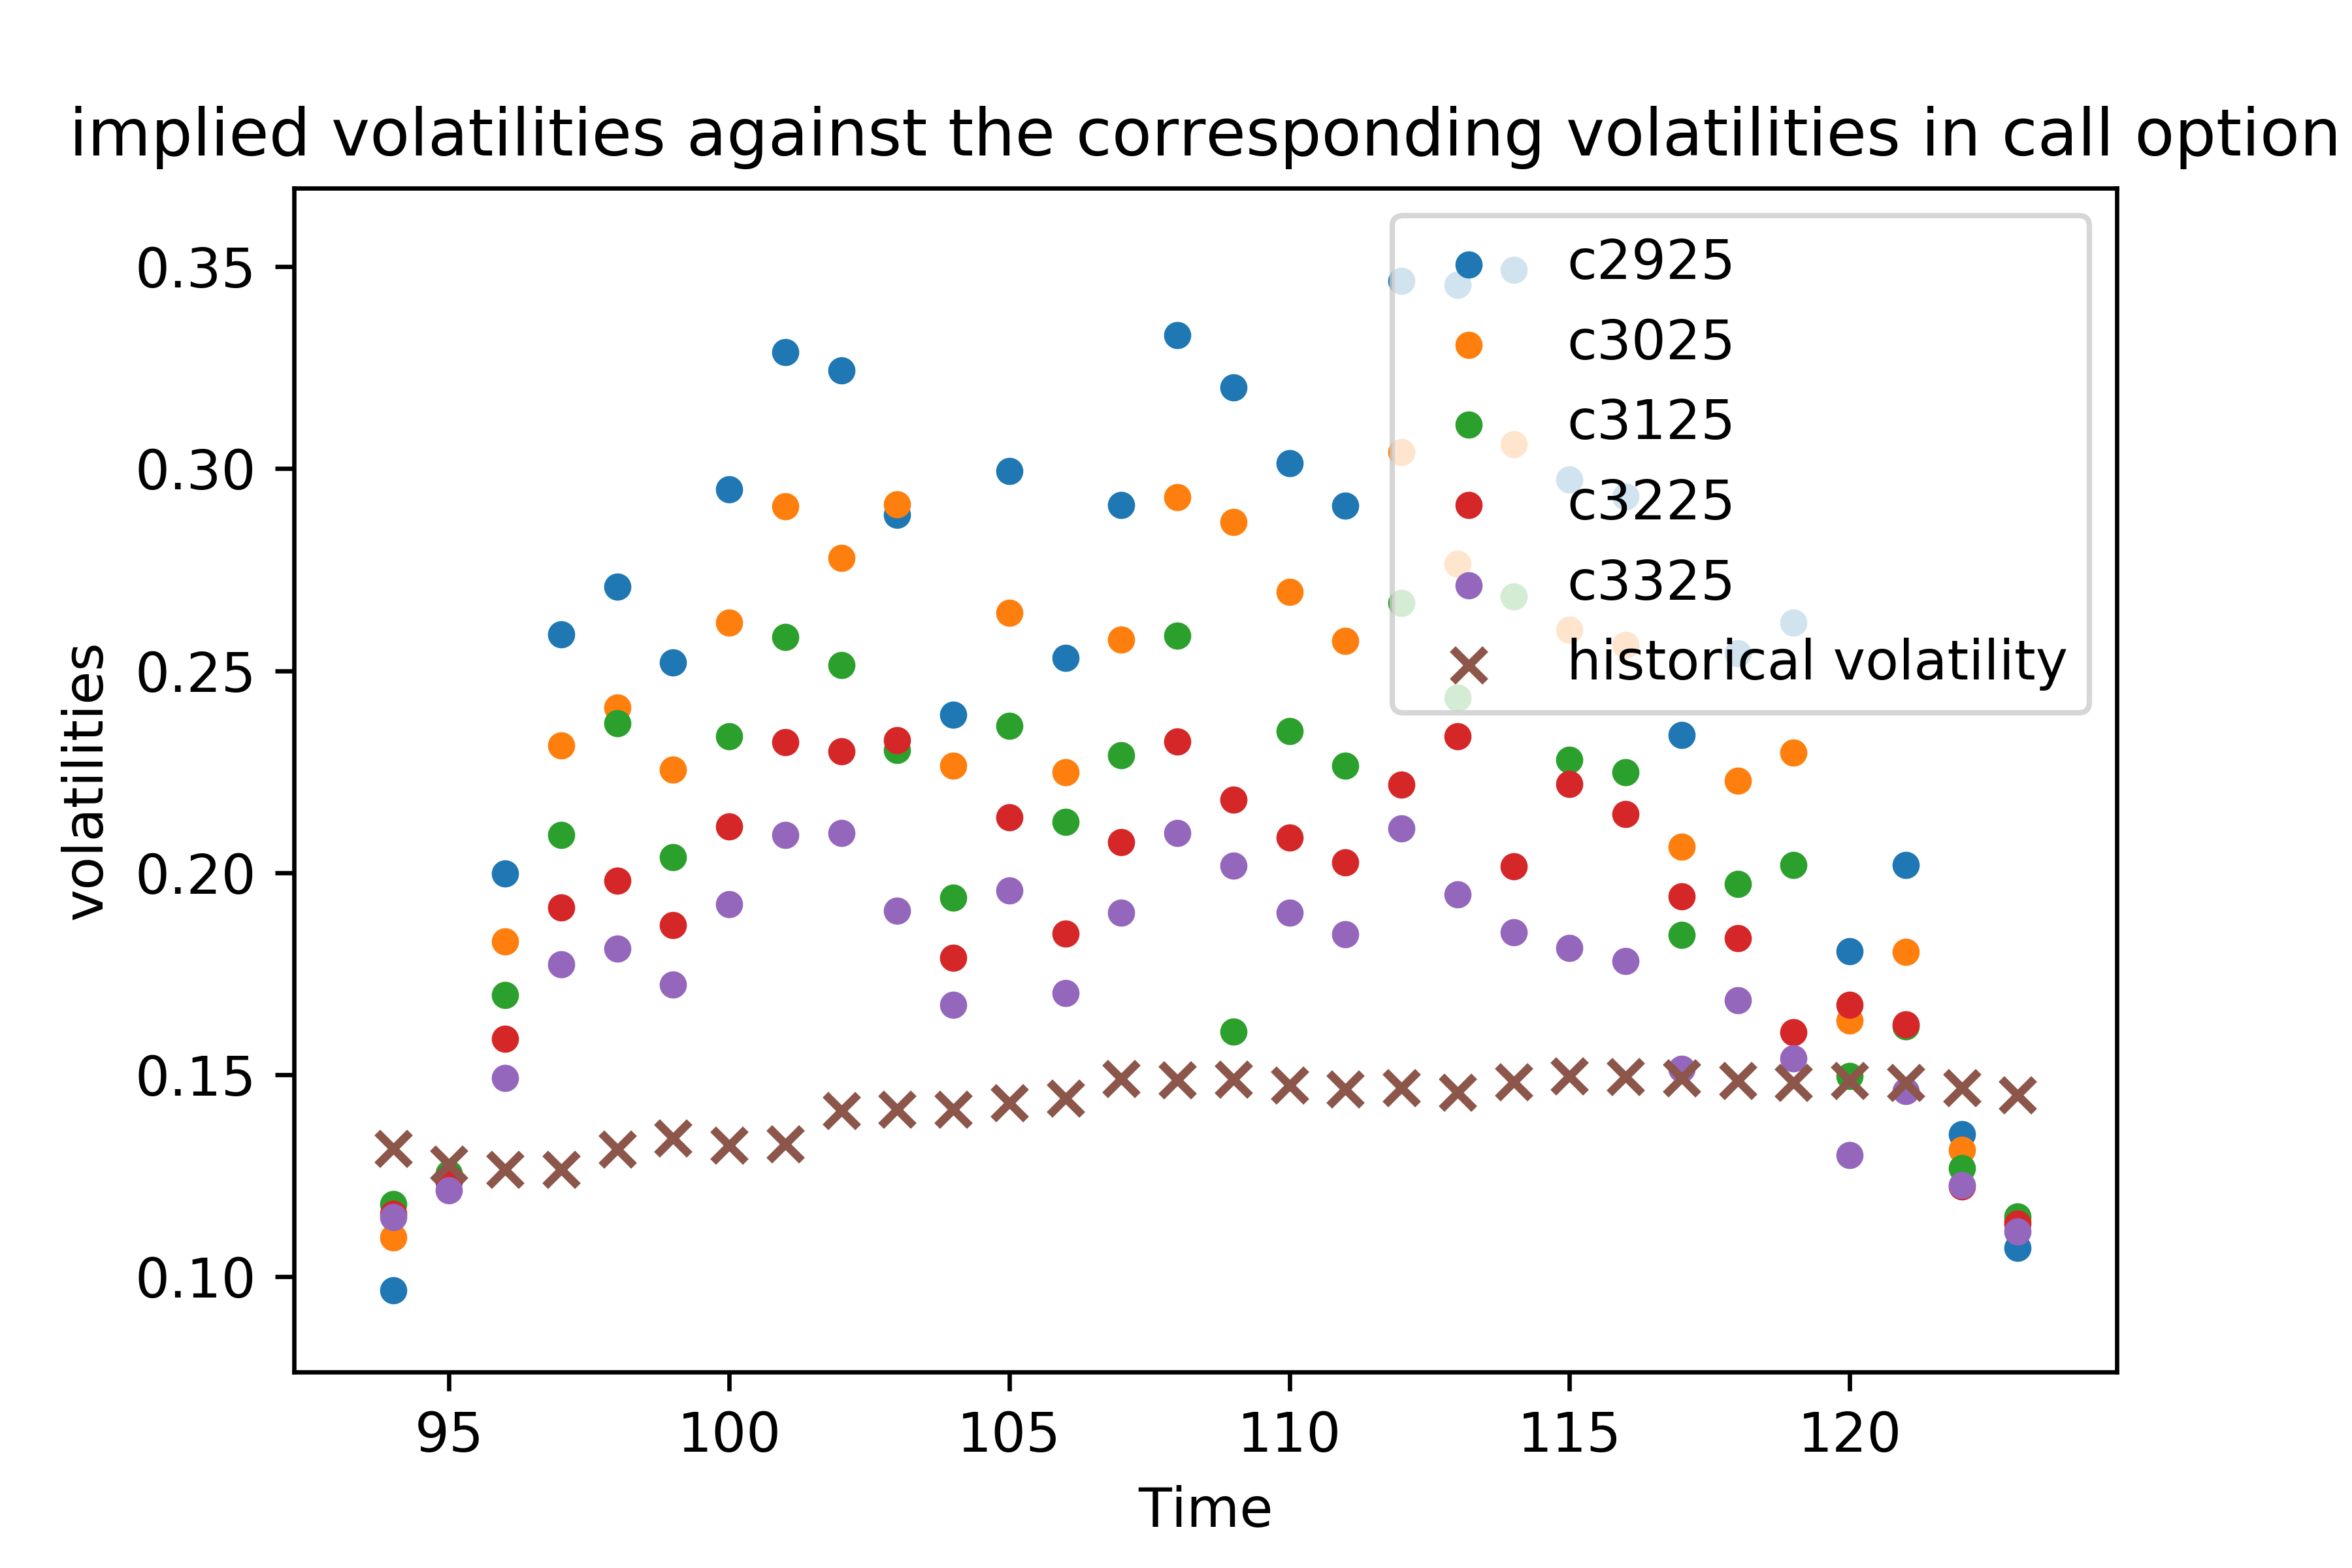
\includegraphics[width=0.50\textwidth]{19.png}
    \caption{\label{}Implied volatilities against the corresponding historical volatilities in call option from day94 to day123}
\end{figure}

\begin{figure}[htbp]
    \centering
    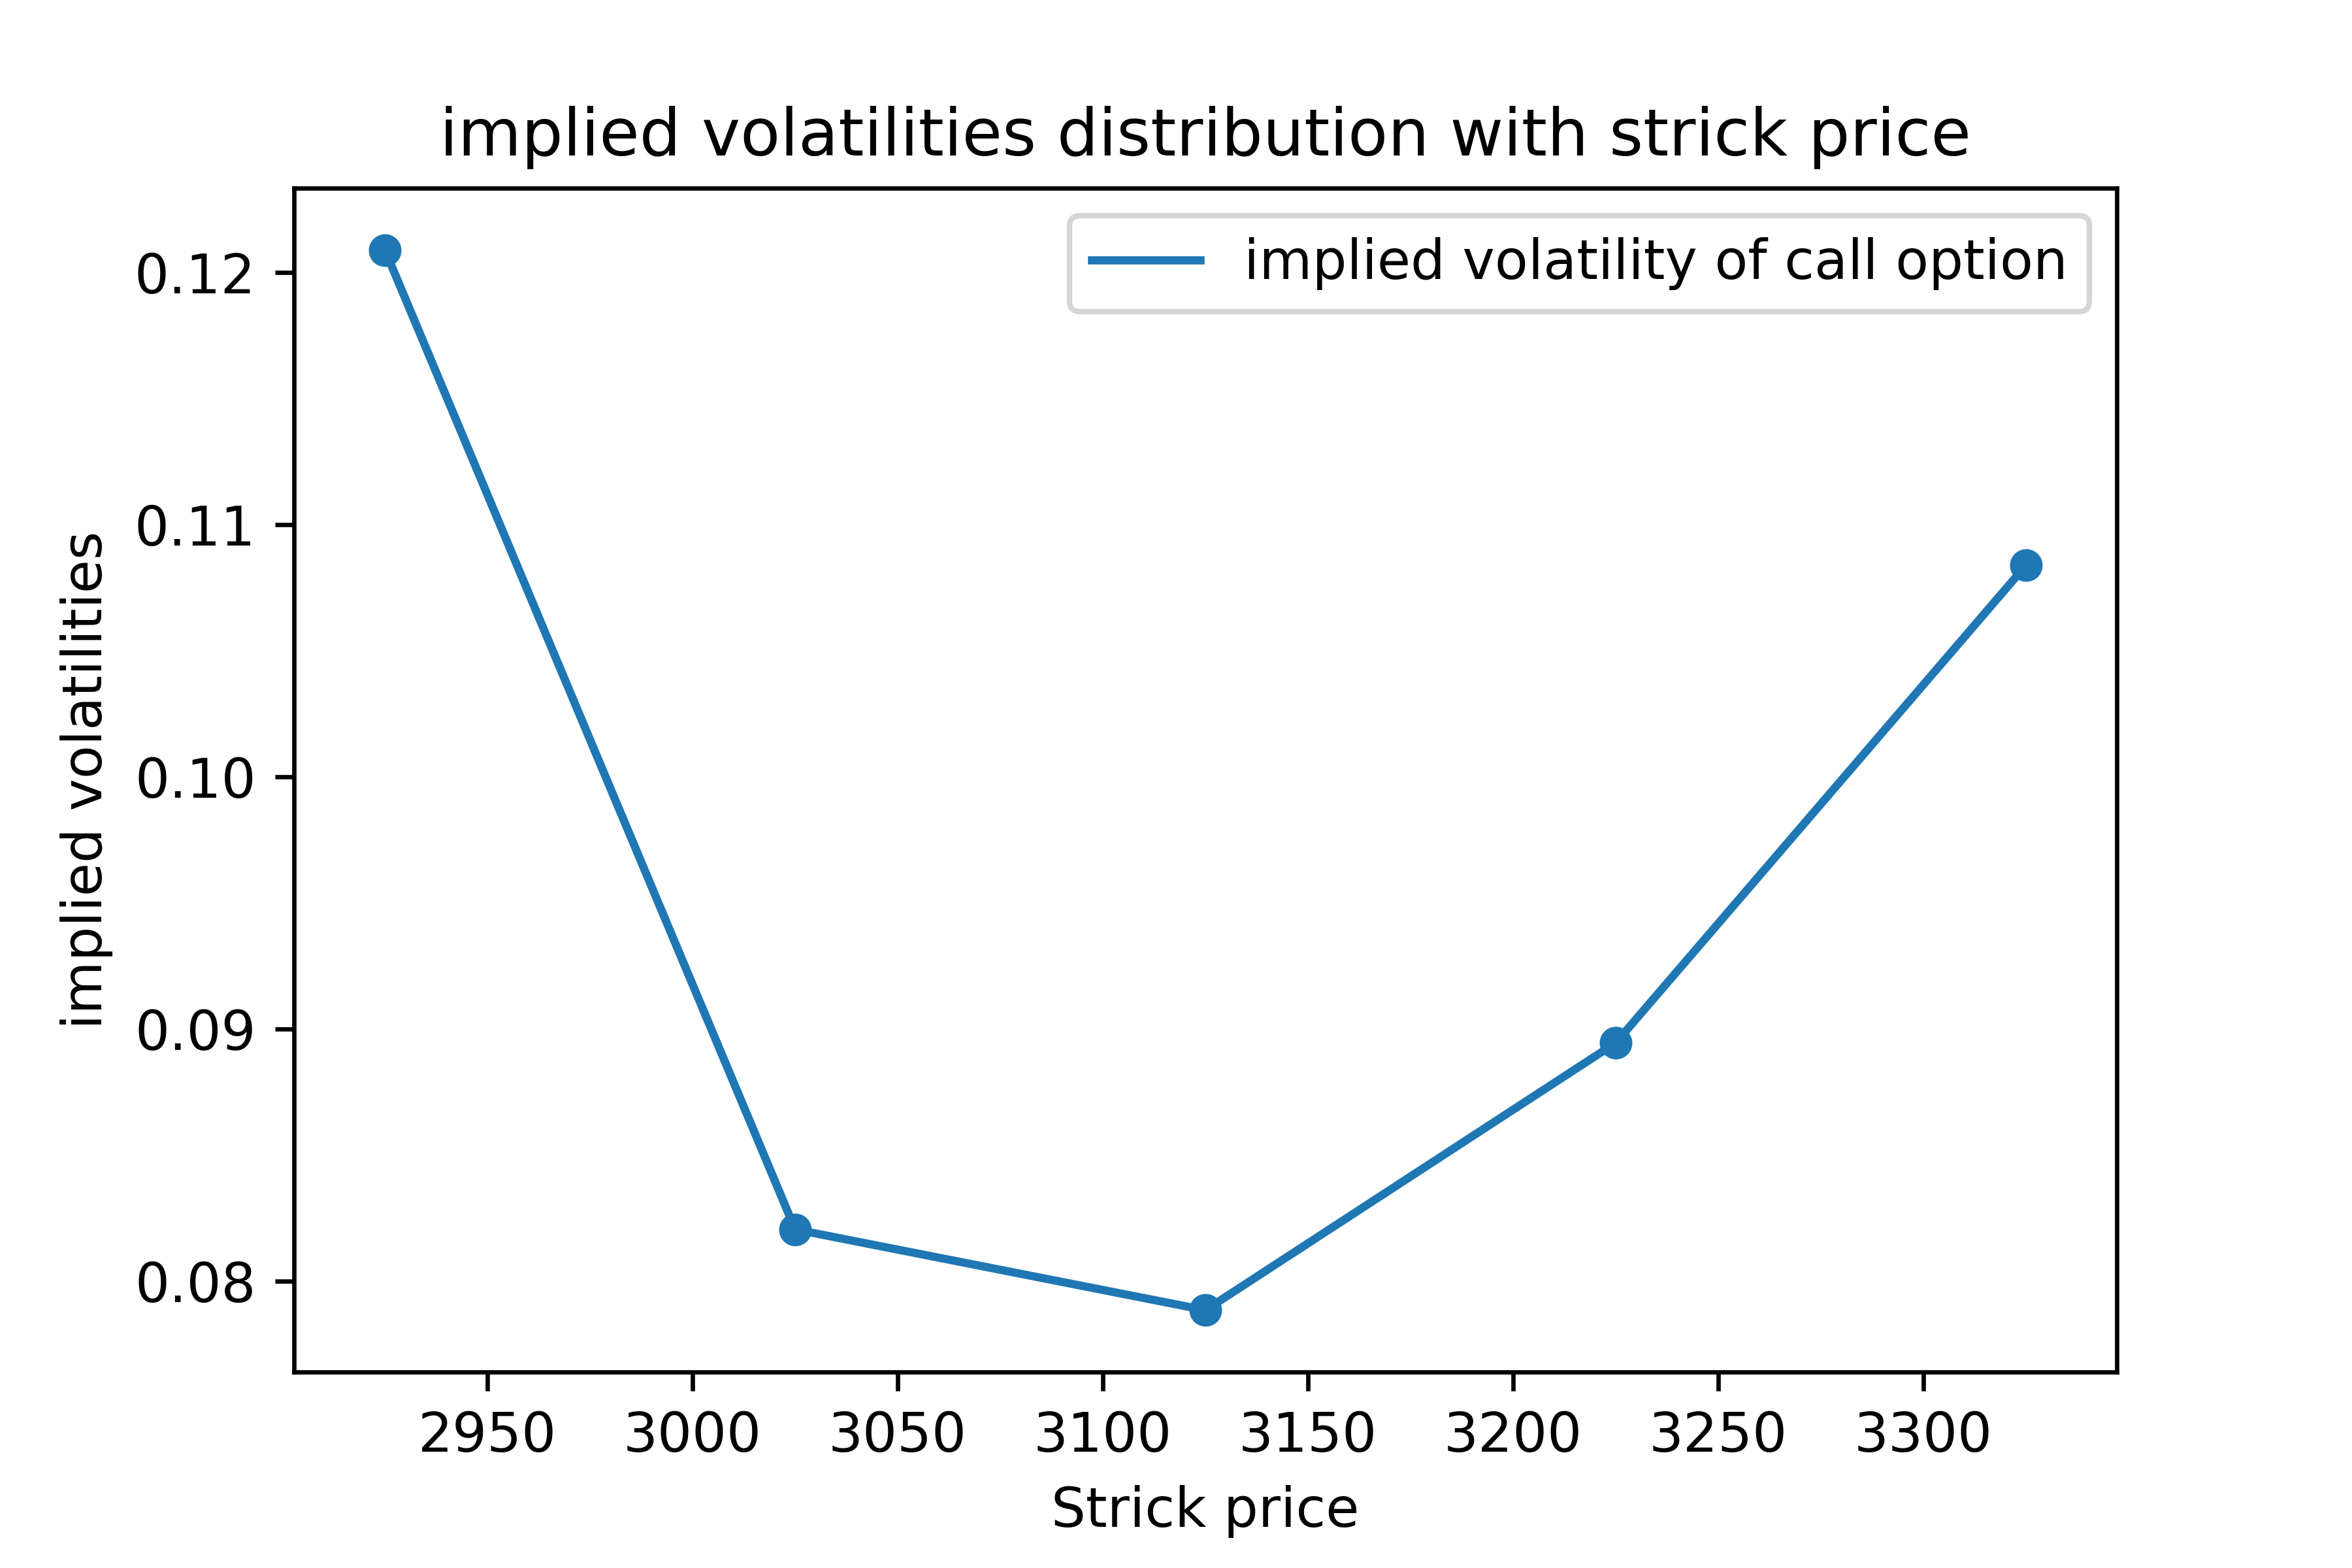
\includegraphics[width=0.50\textwidth]{20.png}
    \caption{\label{}Implied volatilities smile at day 157}
\end{figure}

Since the Black-Scholes option pricing formula is based on the assumption that the underlying asset is subject to a lognormal distribution, this assumption is obviously different from reality. So people use the option price for the same period of different strick price to find the corresponding implied volatility generate curve by them.

Put-call parity $p+S_{0}e^{-qT} = c+Ke^{-rT}$ holds regardless of the assumptions made about the stock price distribution. It follows that $p_{mkt}-p_{bs}=c_{mkt}-c_{bs}$\cite{hull2016options}. Therefore the implied volatility calculated from a European call option should be the same as that calculated from a European put option when both have the same strike price and maturity. The calculated curve is shown in $Fig18$. It could find the implied volatitity has higher value at high and low of strick price which is look like a smile. However, for most of days, the implied volatitity is distribute like strick skew.

Volatility smiles tell people that demand is greater for options that are in-the-money or out-of-the-money. Traders use volatility smiles to allow for nonlognormality. The volatility smile defines the relationship between the implied volatility of an option and its strike price. For equity options, the volatility smile tends to be downward sloping. This means that outof-the-money puts and in-the-money calls tend to have high implied volatilities whereas out-of-the-money calls and in-the-money puts tend to have low implied volatilities\cite{hull2016options}.

%%%%%%%%%%%%%%%%%%%%%%%%%%%%%%%%%%%%%%%%%%%%%%%%%%%%%%%%%%%%%%%%%%%%%%%

\subsection{Question 3}

The binomial option pricing model assumes that the volatility of stocks only have upward and downward directions, in addition, assumes that the probability and amplitude of each changing are invariable during the entire investigation period. The model divides the duration of the investigation into several phases. It simulates all possible development paths of the underlying stock during the entire duration based on the historical volatility of the stock price and calculates the warrants income at each node.

The parameters in this model can be defined as:

\begin{equation} \label{eq46}
\setlength{\abovedisplayskip}{3pt}
\setlength{\belowdisplayskip}{9pt}
\begin{split}
&u = e^{\sigma \sqrt{\delta t}}\\
&d=e^{-\sigma \sqrt{\delta t}}\\
&p=\frac{e^{r\delta t}-d}{u-d}
\end{split}
\end{equation}

Choose $c3025$ as the target stock, it has $S_{0}=3480$, $K=3025$. Randomly set other parameters $r=0.06$, $\sigma=0.5$ and $maturity\ time = 100$. The call option can be calculated by Black-Scholes model and Binomial lattice methods respective. $Fig19$ is the comparison of those two methods, it could find the fluctuation of Binomial lattice method is frequent at the beginning, and it the price will close to Black-Scholes model with the increasing time. $Fig20$ is the absolute difference between two methods with $\delta t$, it could find the absolute difference decreases with the decreasing $\delta t$. ~\\

\begin{figure}[htbp]
    \centering
    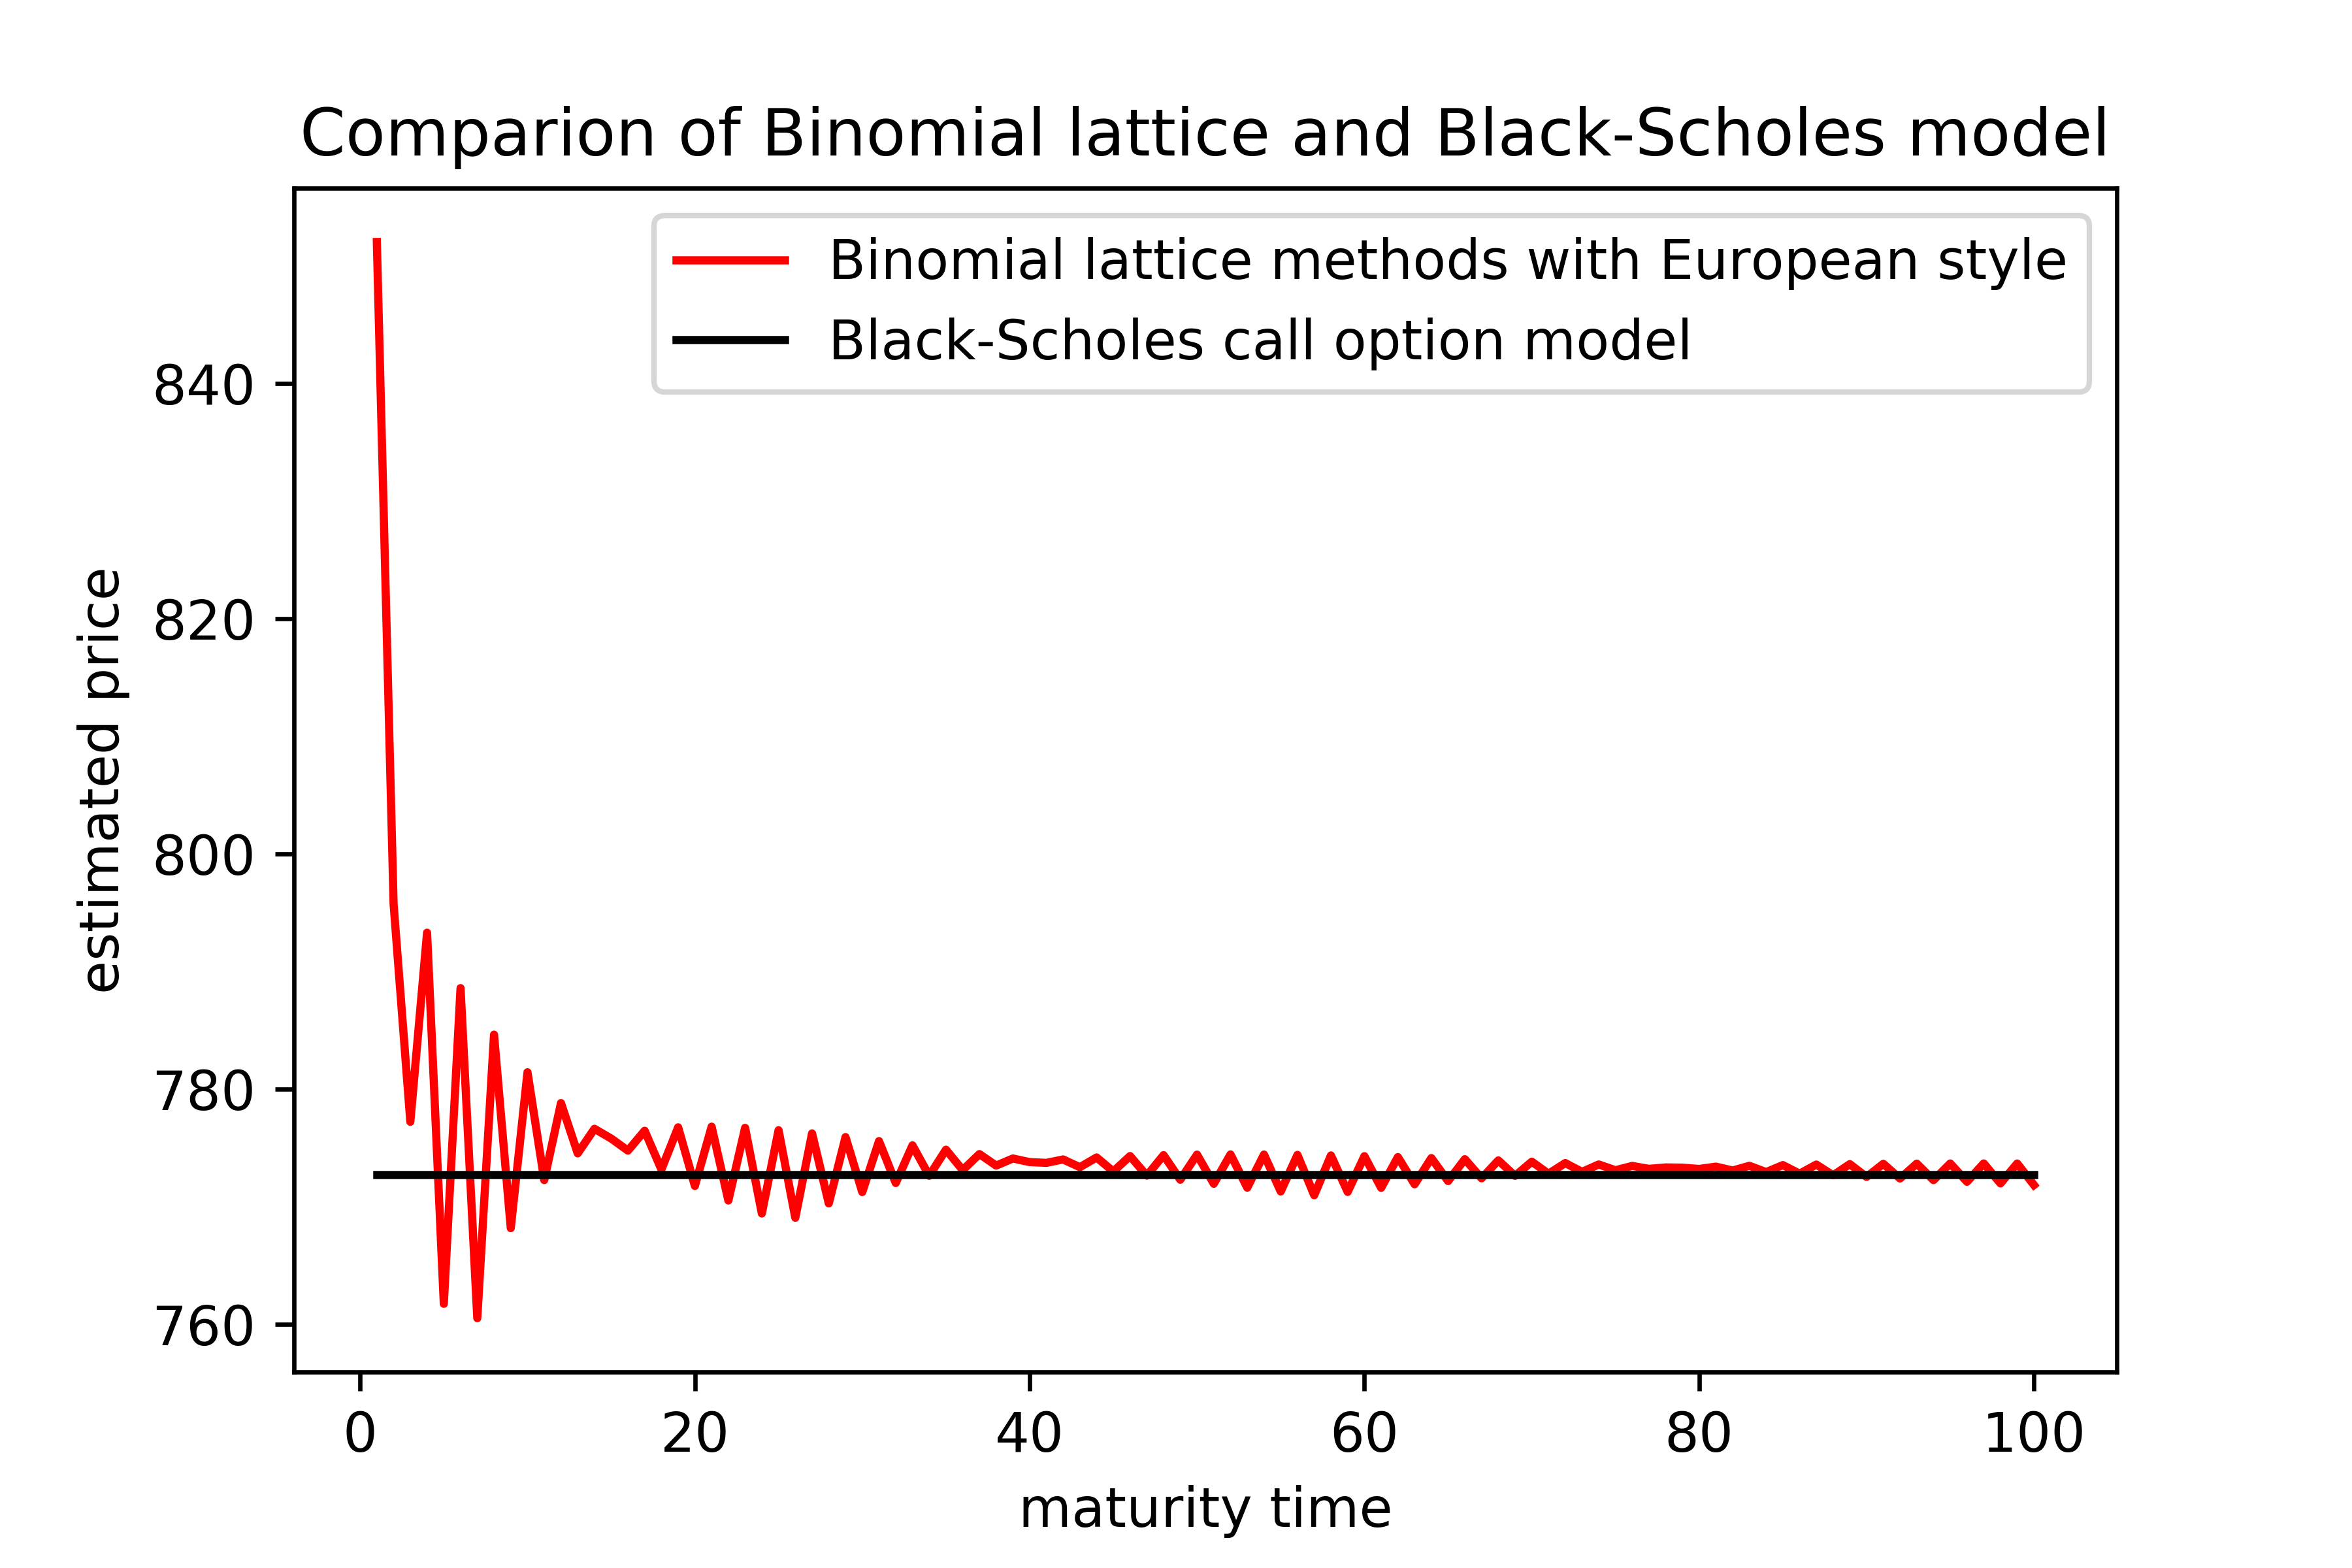
\includegraphics[width=0.50\textwidth]{21.png}
    \caption{\label{}Comparion of Binomial lattice and Black-Scholes model with given parameters}
\end{figure}

\begin{figure}[htbp]
    \centering
    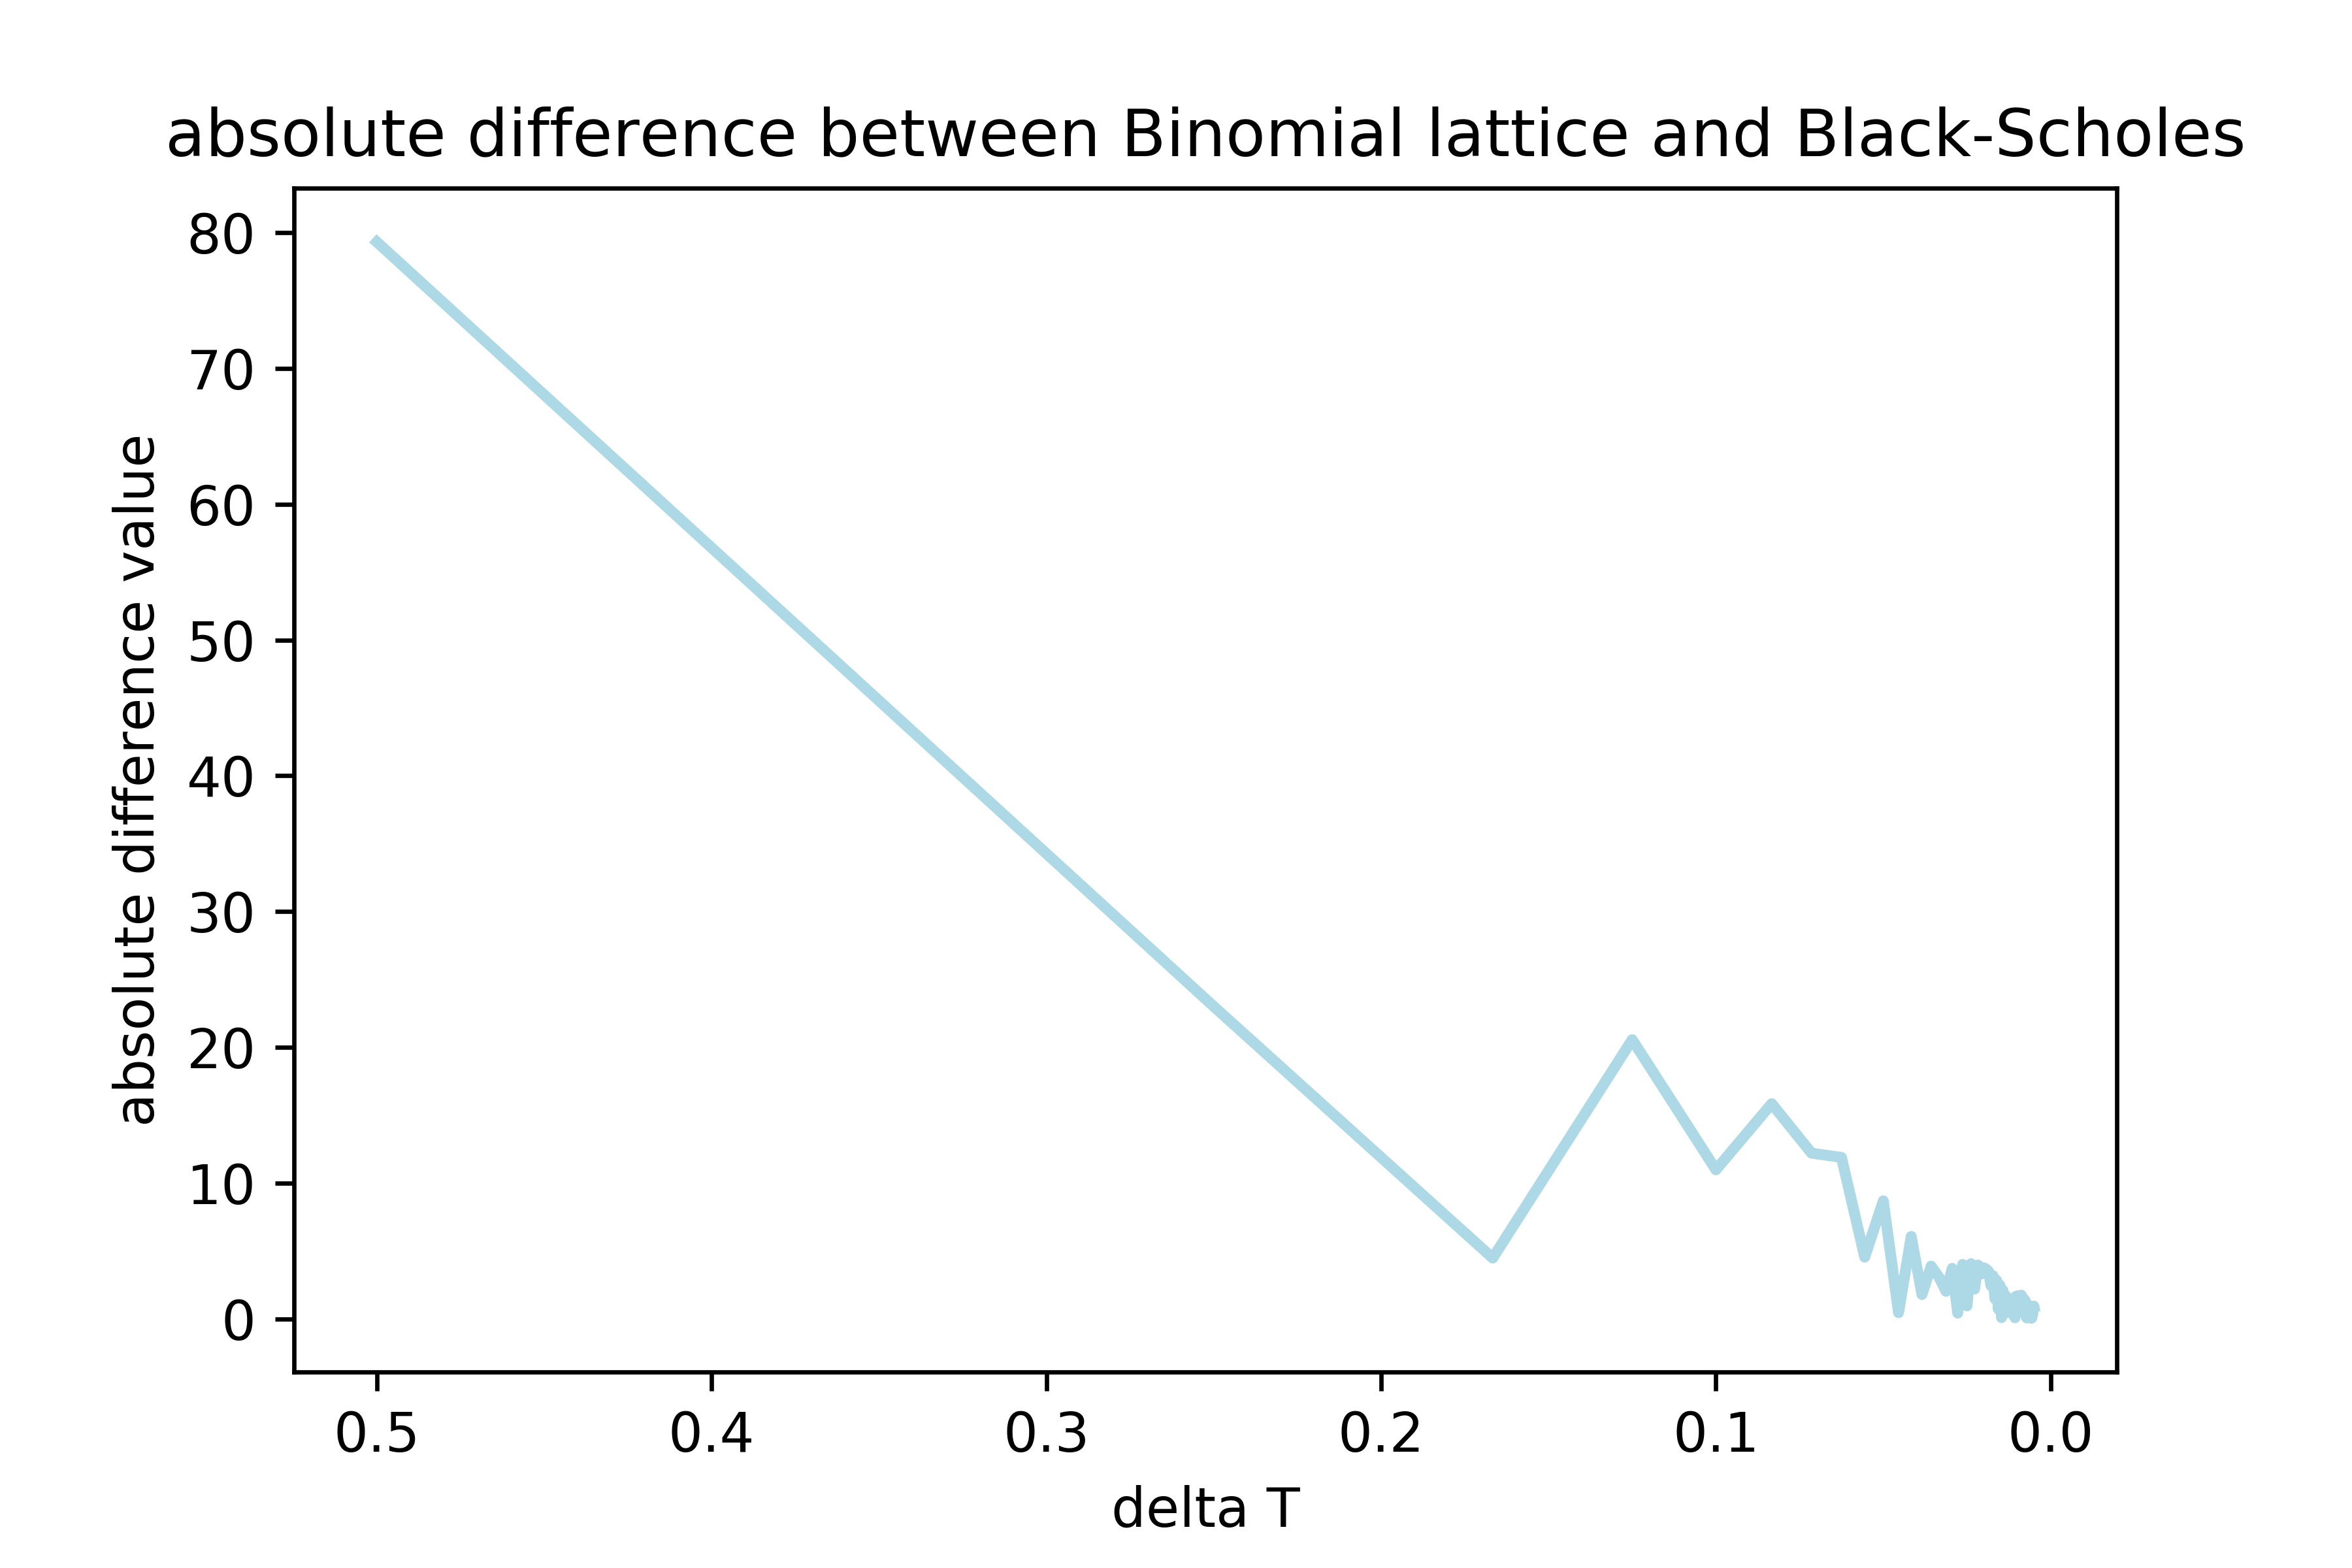
\includegraphics[width=0.50\textwidth]{22.png}
    \caption{\label{}Absolute difference between Binomial lattice and Black-Scholes with given parameters}
\end{figure}

American options are contracts that may be exercised early, prior to expiry. However, The options which contrasted with European options for which exercise is only permitted at expiry. Therefore, the calculation of American option should check each node for early exercise. 

\begin{figure}[htbp]
    \centering
    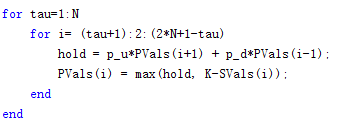
\includegraphics[width=0.35\textwidth]{23.png}
    \caption{\label{}The code for pricing a put option with American style\cite{brandimarte2013numerical}}
\end{figure}

If the call option in American was early exercised, the intrinsic value should be:

\begin{equation} \label{eq47}
\setlength{\abovedisplayskip}{3pt}
\setlength{\belowdisplayskip}{9pt}
PVals_{n}^{m}=max(S_{n}^{m}-K,0) \quad n=0,1,2...,m
\end{equation}

for the put option in American style, it is:

\begin{equation} \label{eq48}
\setlength{\abovedisplayskip}{3pt}
\setlength{\belowdisplayskip}{9pt}
PVals_{n}^{m}=max(K-S_{n}^{m},0) \quad n=0,1,2...,m
\end{equation}

At time node $m\Delta^{t}$, the probability of $(m,n)$ to $(m+1,n+1)$ is $p\_u$, the probability of $(m,n)$ to $(m+1,n)$ is $p\_d$. 

Therefore, if the share option not early exercise, it has:

\begin{equation} \label{eq49}
\setlength{\abovedisplayskip}{3pt}
\setlength{\belowdisplayskip}{9pt}
\begin{split}
&PVals_{n}^{m}=p\_u\times PVals_{m+1}^{m+1}+p\_d\times PVals_{n}^{m+1} \\
&p\_u = e^{-r\delta t}\\
&p\_d = 1 - p\_u
\end{split}
\end{equation}

If the share option early exercise, it should be compared to the intrinsic value which defined as eq\eqref{eq47} and eq\eqref{eq48}. The max value will be used for new lntrinsic value. In $Fig21$ which come from \cite{brandimarte2013numerical}, it could find the hold is the share option and it is the code for put option because the intrinsic function is $(K-SVals(i))$. Therefore, change it for call option with American style is using the intrinsic function of call option $(SVAls(i)-K)$to replace the put option one which can be seen in $Fig22$.

\begin{figure}[htbp]
    \centering
    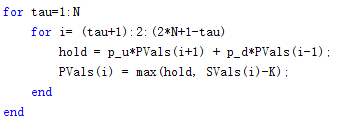
\includegraphics[width=0.35\textwidth]{24.png}
    \caption{\label{}The code for pricing a call option with American style}
\end{figure}

%%%%%%%%%%%%%%%%%%%%%%%%%%%%%%%%%%%%%%%%%%%%%%%%%%%%%%%%%%%%%%%%%%%%%%%
\bibliographystyle{ACM-Reference-Format}
\bibliography{computation_finance}
\end{document}
